\documentclass[twoside]{book}

% Packages required by doxygen
\usepackage{fixltx2e}
\usepackage{calc}
\usepackage{doxygen}
\usepackage[export]{adjustbox} % also loads graphicx
\usepackage{graphicx}
\usepackage[utf8]{inputenc}
\usepackage{makeidx}
\usepackage{multicol}
\usepackage{multirow}
\PassOptionsToPackage{warn}{textcomp}
\usepackage{textcomp}
\usepackage[nointegrals]{wasysym}
\usepackage[table]{xcolor}

% Font selection
\usepackage[T1]{fontenc}
\usepackage[scaled=.90]{helvet}
\usepackage{courier}
\usepackage{amssymb}
\usepackage{sectsty}
\renewcommand{\familydefault}{\sfdefault}
\allsectionsfont{%
  \fontseries{bc}\selectfont%
  \color{darkgray}%
}
\renewcommand{\DoxyLabelFont}{%
  \fontseries{bc}\selectfont%
  \color{darkgray}%
}
\newcommand{\+}{\discretionary{\mbox{\scriptsize$\hookleftarrow$}}{}{}}

% Page & text layout
\usepackage{geometry}
\geometry{%
  a4paper,%
  top=2.5cm,%
  bottom=2.5cm,%
  left=2.5cm,%
  right=2.5cm%
}
\tolerance=750
\hfuzz=15pt
\hbadness=750
\setlength{\emergencystretch}{15pt}
\setlength{\parindent}{0cm}
\setlength{\parskip}{3ex plus 2ex minus 2ex}
\makeatletter
\renewcommand{\paragraph}{%
  \@startsection{paragraph}{4}{0ex}{-1.0ex}{1.0ex}{%
    \normalfont\normalsize\bfseries\SS@parafont%
  }%
}
\renewcommand{\subparagraph}{%
  \@startsection{subparagraph}{5}{0ex}{-1.0ex}{1.0ex}{%
    \normalfont\normalsize\bfseries\SS@subparafont%
  }%
}
\makeatother

% Headers & footers
\usepackage{fancyhdr}
\pagestyle{fancyplain}
\fancyhead[LE]{\fancyplain{}{\bfseries\thepage}}
\fancyhead[CE]{\fancyplain{}{}}
\fancyhead[RE]{\fancyplain{}{\bfseries\leftmark}}
\fancyhead[LO]{\fancyplain{}{\bfseries\rightmark}}
\fancyhead[CO]{\fancyplain{}{}}
\fancyhead[RO]{\fancyplain{}{\bfseries\thepage}}
\fancyfoot[LE]{\fancyplain{}{}}
\fancyfoot[CE]{\fancyplain{}{}}
\fancyfoot[RE]{\fancyplain{}{\bfseries\scriptsize Generated by Doxygen }}
\fancyfoot[LO]{\fancyplain{}{\bfseries\scriptsize Generated by Doxygen }}
\fancyfoot[CO]{\fancyplain{}{}}
\fancyfoot[RO]{\fancyplain{}{}}
\renewcommand{\footrulewidth}{0.4pt}
\renewcommand{\chaptermark}[1]{%
  \markboth{#1}{}%
}
\renewcommand{\sectionmark}[1]{%
  \markright{\thesection\ #1}%
}

% Indices & bibliography
\usepackage{natbib}
\usepackage[titles]{tocloft}
\setcounter{tocdepth}{3}
\setcounter{secnumdepth}{5}
\makeindex

% Hyperlinks (required, but should be loaded last)
\usepackage{ifpdf}
\ifpdf
  \usepackage[pdftex,pagebackref=true]{hyperref}
\else
  \usepackage[ps2pdf,pagebackref=true]{hyperref}
\fi
\hypersetup{%
  colorlinks=true,%
  linkcolor=blue,%
  citecolor=blue,%
  unicode%
}

% Custom commands
\newcommand{\clearemptydoublepage}{%
  \newpage{\pagestyle{empty}\cleardoublepage}%
}

\usepackage{caption}
\captionsetup{labelsep=space,justification=centering,font={bf},singlelinecheck=off,skip=4pt,position=top}

%===== C O N T E N T S =====

\begin{document}

% Titlepage & ToC
\hypersetup{pageanchor=false,
             bookmarksnumbered=true,
             pdfencoding=unicode
            }
\pagenumbering{alph}
\begin{titlepage}
\vspace*{7cm}
\begin{center}%
{\Large D\+R\+O\+N\+NN \\[1ex]\large 1.\+0 }\\
\vspace*{1cm}
{\large Generated by Doxygen 1.8.13}\\
\end{center}
\end{titlepage}
\clearemptydoublepage
\pagenumbering{roman}
\tableofcontents
\clearemptydoublepage
\pagenumbering{arabic}
\hypersetup{pageanchor=true}

%--- Begin generated contents ---
\chapter{Namespace Index}
\section{Namespace List}
Here is a list of all namespaces with brief descriptions\+:\begin{DoxyCompactList}
\item\contentsline{section}{\hyperlink{namespace_pz_g}{PzG} \\*Moduł narzędzi umożliwiających połącznie z G\+N\+U\+Plotem }{\pageref{namespace_pz_g}}{}
\end{DoxyCompactList}

\chapter{Hierarchical Index}
\section{Class Hierarchy}
This inheritance list is sorted roughly, but not completely, alphabetically\+:\begin{DoxyCompactList}
\item \contentsline{section}{PzG\+:\+:Info\+Pliku\+Do\+Rysowania}{\pageref{class_pz_g_1_1_info_pliku_do_rysowania}}{}
\item \contentsline{section}{PzG\+:\+:Lacze\+Do\+G\+N\+U\+Plota}{\pageref{class_pz_g_1_1_lacze_do_g_n_u_plota}}{}
\item \contentsline{section}{Macierz$<$ Wymiar $>$}{\pageref{class_macierz}}{}
\item \contentsline{section}{Obj\+\_\+\+Geo}{\pageref{class_obj___geo}}{}
\begin{DoxyCompactList}
\item \contentsline{section}{Prostopadloscian}{\pageref{class_prostopadloscian}}{}
\begin{DoxyCompactList}
\item \contentsline{section}{Obstacle}{\pageref{class_obstacle}}{}
\end{DoxyCompactList}
\item \contentsline{section}{Rotor}{\pageref{class_rotor}}{}
\end{DoxyCompactList}
\item \contentsline{section}{Obj\+\_\+\+Sc}{\pageref{class_obj___sc}}{}
\begin{DoxyCompactList}
\item \contentsline{section}{Dron}{\pageref{class_dron}}{}
\item \contentsline{section}{Obstacle}{\pageref{class_obstacle}}{}
\end{DoxyCompactList}
\item \contentsline{section}{Scena}{\pageref{class_scena}}{}
\item \contentsline{section}{Wektor$<$ Wymiar $>$}{\pageref{class_wektor}}{}
\item \contentsline{section}{Wektor$<$ 3 $>$}{\pageref{class_wektor}}{}
\end{DoxyCompactList}

\chapter{Class Index}
\section{Class List}
Here are the classes, structs, unions and interfaces with brief descriptions\+:\begin{DoxyCompactList}
\item\contentsline{section}{\hyperlink{class_dron}{Dron} \\*Klasa określa współrzędne rotorów oraz korpusu. Jest fragmentem objektu sceny }{\pageref{class_dron}}{}
\item\contentsline{section}{\hyperlink{class_pz_g_1_1_info_pliku_do_rysowania}{Pz\+G\+::\+Info\+Pliku\+Do\+Rysowania} \\*Zestaw informacji dotyczący pliku i sposobu rysowania }{\pageref{class_pz_g_1_1_info_pliku_do_rysowania}}{}
\item\contentsline{section}{\hyperlink{class_pz_g_1_1_lacze_do_g_n_u_plota}{Pz\+G\+::\+Lacze\+Do\+G\+N\+U\+Plota} \\*Klasa realizuje interfejs do programu G\+N\+U\+Plot }{\pageref{class_pz_g_1_1_lacze_do_g_n_u_plota}}{}
\item\contentsline{section}{\hyperlink{class_macierz}{Macierz$<$ Wymiar $>$} \\*Klasa ta reprezentuje macierz (tablica n-\/wymiarowa, metoda rotacji, przeciążenia operatorów itp) }{\pageref{class_macierz}}{}
\item\contentsline{section}{\hyperlink{class_obj___geo}{Obj\+\_\+\+Geo} }{\pageref{class_obj___geo}}{}
\item\contentsline{section}{\hyperlink{class_obj___sc}{Obj\+\_\+\+Sc} \\*Klasa ta jest dziedziczona do drona oraz przeszkody. Jego metodą jest wykrywanie kolizji }{\pageref{class_obj___sc}}{}
\item\contentsline{section}{\hyperlink{class_obstacle}{Obstacle} \\*Klasa określa przeszkode. Jest fragmentem objektu sceny }{\pageref{class_obstacle}}{}
\item\contentsline{section}{\hyperlink{class_prostopadloscian}{Prostopadloscian} \\*Klasa ta reprezentuje prostopadłościan oraz to co go określa (współrzędne, metody obrotu, translacji itp) }{\pageref{class_prostopadloscian}}{}
\item\contentsline{section}{\hyperlink{class_rotor}{Rotor} \\*Klasa określa współrzędne rotorów oraz jak się obracają }{\pageref{class_rotor}}{}
\item\contentsline{section}{\hyperlink{class_scena}{Scena} \\*Klasa ta reprezentuje scene. Jego polami to lista objektów scen oraz dronów }{\pageref{class_scena}}{}
\item\contentsline{section}{\hyperlink{class_wektor}{Wektor$<$ Wymiar $>$} \\*Klasa ta reprezentuje wektor (tablica n-\/wymiarowa, przeciążenia operatorów itp) }{\pageref{class_wektor}}{}
\end{DoxyCompactList}

\chapter{File Index}
\section{File List}
Here is a list of all files with brief descriptions\+:\begin{DoxyCompactList}
\item\contentsline{section}{inc/\hyperlink{_dron_8hh}{Dron.\+hh} }{\pageref{_dron_8hh}}{}
\item\contentsline{section}{inc/\hyperlink{lacze__do__gnuplota_8hh}{lacze\+\_\+do\+\_\+gnuplota.\+hh} }{\pageref{lacze__do__gnuplota_8hh}}{}
\item\contentsline{section}{inc/\hyperlink{_macierz_8hh}{Macierz.\+hh} }{\pageref{_macierz_8hh}}{}
\item\contentsline{section}{inc/\hyperlink{_macierz3x3_8hh}{Macierz3x3.\+hh} }{\pageref{_macierz3x3_8hh}}{}
\item\contentsline{section}{inc/\hyperlink{_obj___geo_8hh}{Obj\+\_\+\+Geo.\+hh} }{\pageref{_obj___geo_8hh}}{}
\item\contentsline{section}{inc/\hyperlink{_obj___sc_8hh}{Obj\+\_\+\+Sc.\+hh} }{\pageref{_obj___sc_8hh}}{}
\item\contentsline{section}{inc/\hyperlink{_obstacle_8hh}{Obstacle.\+hh} }{\pageref{_obstacle_8hh}}{}
\item\contentsline{section}{inc/\hyperlink{_prostopadloscian_8hh}{Prostopadloscian.\+hh} }{\pageref{_prostopadloscian_8hh}}{}
\item\contentsline{section}{inc/\hyperlink{_rotor_8hh}{Rotor.\+hh} }{\pageref{_rotor_8hh}}{}
\item\contentsline{section}{inc/\hyperlink{_scena_8hh}{Scena.\+hh} }{\pageref{_scena_8hh}}{}
\item\contentsline{section}{inc/\hyperlink{_wektor_8hh}{Wektor.\+hh} }{\pageref{_wektor_8hh}}{}
\item\contentsline{section}{inc/\hyperlink{_wektor3_d_8hh}{Wektor3\+D.\+hh} }{\pageref{_wektor3_d_8hh}}{}
\item\contentsline{section}{src/\hyperlink{_dron_8cpp}{Dron.\+cpp} }{\pageref{_dron_8cpp}}{}
\item\contentsline{section}{src/\hyperlink{lacze__do__gnuplota_8cpp}{lacze\+\_\+do\+\_\+gnuplota.\+cpp} }{\pageref{lacze__do__gnuplota_8cpp}}{}
\item\contentsline{section}{src/\hyperlink{_macierz3x3_8cpp}{Macierz3x3.\+cpp} }{\pageref{_macierz3x3_8cpp}}{}
\item\contentsline{section}{src/\hyperlink{main_8cpp}{main.\+cpp} }{\pageref{main_8cpp}}{}
\item\contentsline{section}{src/\hyperlink{_obj___geo_8cpp}{Obj\+\_\+\+Geo.\+cpp} }{\pageref{_obj___geo_8cpp}}{}
\item\contentsline{section}{src/\hyperlink{_obj___sc_8cpp}{Obj\+\_\+\+Sc.\+cpp} }{\pageref{_obj___sc_8cpp}}{}
\item\contentsline{section}{src/\hyperlink{_obstacle_8cpp}{Obstacle.\+cpp} }{\pageref{_obstacle_8cpp}}{}
\item\contentsline{section}{src/\hyperlink{_prostopadloscian_8cpp}{Prostopadloscian.\+cpp} }{\pageref{_prostopadloscian_8cpp}}{}
\item\contentsline{section}{src/\hyperlink{_rotor_8cpp}{Rotor.\+cpp} }{\pageref{_rotor_8cpp}}{}
\item\contentsline{section}{src/\hyperlink{_scena_8cpp}{Scena.\+cpp} }{\pageref{_scena_8cpp}}{}
\item\contentsline{section}{src/\hyperlink{_wektor3_d_8cpp}{Wektor3\+D.\+cpp} }{\pageref{_wektor3_d_8cpp}}{}
\end{DoxyCompactList}

\chapter{Namespace Documentation}
\hypertarget{namespace_pz_g}{}\section{PzG Namespace Reference}
\label{namespace_pz_g}\index{PzG@{PzG}}


Moduł narzędzi umożliwiających połącznie z G\+N\+U\+Plotem.  


\subsection*{Classes}
\begin{DoxyCompactItemize}
\item 
class \hyperlink{class_pz_g_1_1_info_pliku_do_rysowania}{Info\+Pliku\+Do\+Rysowania}
\begin{DoxyCompactList}\small\item\em Zestaw informacji dotyczący pliku i sposobu rysowania. \end{DoxyCompactList}\item 
class \hyperlink{class_pz_g_1_1_lacze_do_g_n_u_plota}{Lacze\+Do\+G\+N\+U\+Plota}
\begin{DoxyCompactList}\small\item\em Klasa realizuje interfejs do programu G\+N\+U\+Plot. \end{DoxyCompactList}\end{DoxyCompactItemize}
\subsection*{Enumerations}
\begin{DoxyCompactItemize}
\item 
enum \hyperlink{namespace_pz_g_aeedae1ef10c66d720f9e89de408ca4ca}{Tryb\+Rysowania} \{ \hyperlink{namespace_pz_g_aeedae1ef10c66d720f9e89de408ca4caa5eb0cf8b3405e136f092efdb489d60c4}{T\+R\+\_\+2D}, 
\hyperlink{namespace_pz_g_aeedae1ef10c66d720f9e89de408ca4caa856e6b0fa6b8a9dc184c60cf27dcc5d2}{T\+R\+\_\+3D}
 \}\begin{DoxyCompactList}\small\item\em Określa tryb rysowania realizowanego przez program {\ttfamily gnuplot}. \end{DoxyCompactList}
\item 
enum \hyperlink{namespace_pz_g_a705c92106f39b7d0c34a6739d10ff0b6}{Rodzaj\+Rysowania} \{ \hyperlink{namespace_pz_g_a705c92106f39b7d0c34a6739d10ff0b6a927eaa159aa4bd3198f0a330b967746d}{R\+R\+\_\+\+Ciagly}, 
\hyperlink{namespace_pz_g_a705c92106f39b7d0c34a6739d10ff0b6aa01097ee8266d6402b752ef6f9a4690c}{R\+R\+\_\+\+Punktowy}
 \}\begin{DoxyCompactList}\small\item\em Sposób rysowania linii. \end{DoxyCompactList}
\end{DoxyCompactItemize}
\subsection*{Functions}
\begin{DoxyCompactItemize}
\item 
bool \hyperlink{namespace_pz_g_ae1ae4d36f66c77879380ba73da8e20e3}{Czy\+Jest\+Plik} (char const $\ast$Nazwa\+Pliku)
\end{DoxyCompactItemize}


\subsection{Detailed Description}
Moduł narzędzi umożliwiających połącznie z G\+N\+U\+Plotem. 

Niniejsza przestrzeń nazw stanowi moduł logiczny zawierający narzędzia umożliwiające realizację połączenia z programem {\ttfamily gnuplot}. 

\subsection{Enumeration Type Documentation}
\mbox{\Hypertarget{namespace_pz_g_a705c92106f39b7d0c34a6739d10ff0b6}\label{namespace_pz_g_a705c92106f39b7d0c34a6739d10ff0b6}} 
\index{PzG@{PzG}!Rodzaj\+Rysowania@{Rodzaj\+Rysowania}}
\index{Rodzaj\+Rysowania@{Rodzaj\+Rysowania}!PzG@{PzG}}
\subsubsection{\texorpdfstring{Rodzaj\+Rysowania}{RodzajRysowania}}
{\footnotesize\ttfamily enum \hyperlink{namespace_pz_g_a705c92106f39b7d0c34a6739d10ff0b6}{Pz\+G\+::\+Rodzaj\+Rysowania}}



Sposób rysowania linii. 

Określa sposób rysowania linii. \begin{DoxyEnumFields}{Enumerator}
\raisebox{\heightof{T}}[0pt][0pt]{\index{R\+R\+\_\+\+Ciagly@{R\+R\+\_\+\+Ciagly}!PzG@{PzG}}\index{PzG@{PzG}!R\+R\+\_\+\+Ciagly@{R\+R\+\_\+\+Ciagly}}}\mbox{\Hypertarget{namespace_pz_g_a705c92106f39b7d0c34a6739d10ff0b6a927eaa159aa4bd3198f0a330b967746d}\label{namespace_pz_g_a705c92106f39b7d0c34a6739d10ff0b6a927eaa159aa4bd3198f0a330b967746d}} 
R\+R\+\_\+\+Ciagly&\\
\hline

\raisebox{\heightof{T}}[0pt][0pt]{\index{R\+R\+\_\+\+Punktowy@{R\+R\+\_\+\+Punktowy}!PzG@{PzG}}\index{PzG@{PzG}!R\+R\+\_\+\+Punktowy@{R\+R\+\_\+\+Punktowy}}}\mbox{\Hypertarget{namespace_pz_g_a705c92106f39b7d0c34a6739d10ff0b6aa01097ee8266d6402b752ef6f9a4690c}\label{namespace_pz_g_a705c92106f39b7d0c34a6739d10ff0b6aa01097ee8266d6402b752ef6f9a4690c}} 
R\+R\+\_\+\+Punktowy&\\
\hline

\end{DoxyEnumFields}


Definition at line 48 of file lacze\+\_\+do\+\_\+gnuplota.\+hh.

\mbox{\Hypertarget{namespace_pz_g_aeedae1ef10c66d720f9e89de408ca4ca}\label{namespace_pz_g_aeedae1ef10c66d720f9e89de408ca4ca}} 
\index{PzG@{PzG}!Tryb\+Rysowania@{Tryb\+Rysowania}}
\index{Tryb\+Rysowania@{Tryb\+Rysowania}!PzG@{PzG}}
\subsubsection{\texorpdfstring{Tryb\+Rysowania}{TrybRysowania}}
{\footnotesize\ttfamily enum \hyperlink{namespace_pz_g_aeedae1ef10c66d720f9e89de408ca4ca}{Pz\+G\+::\+Tryb\+Rysowania}}



Określa tryb rysowania realizowanego przez program {\ttfamily gnuplot}. 

Typ wyliczeniowy określające dopuszczalne tryby rysowania realizowanego przez program {\ttfamily gnuplot}. Wybór trybu wiąże się ze zmianą sposobu interpretacji danych zawartych pliku. Jeśli np. wybrany zostanie tryb 2D, to zakłada się, że w każdej linii pliku z danymi znajdują się wartości współrzędnych {\itshape x}, {\itshape y}. Wartości typu\+: \begin{DoxyItemize}
\item {\ttfamily T\+R\+\_\+2D} -\/ rysowanie w trybie 2D, co sprowadza się do rysowania wykresów funkcji jednej zmiennej. \item {\ttfamily T\+R\+\_\+3D} -\/ rysowanie w trybie 3D. Oznacza to możliwość rysowania wykresów funkcji dwóch zmiennych. \end{DoxyItemize}
\begin{DoxyEnumFields}{Enumerator}
\raisebox{\heightof{T}}[0pt][0pt]{\index{T\+R\+\_\+2D@{T\+R\+\_\+2D}!PzG@{PzG}}\index{PzG@{PzG}!T\+R\+\_\+2D@{T\+R\+\_\+2D}}}\mbox{\Hypertarget{namespace_pz_g_aeedae1ef10c66d720f9e89de408ca4caa5eb0cf8b3405e136f092efdb489d60c4}\label{namespace_pz_g_aeedae1ef10c66d720f9e89de408ca4caa5eb0cf8b3405e136f092efdb489d60c4}} 
T\+R\+\_\+2D&\\
\hline

\raisebox{\heightof{T}}[0pt][0pt]{\index{T\+R\+\_\+3D@{T\+R\+\_\+3D}!PzG@{PzG}}\index{PzG@{PzG}!T\+R\+\_\+3D@{T\+R\+\_\+3D}}}\mbox{\Hypertarget{namespace_pz_g_aeedae1ef10c66d720f9e89de408ca4caa856e6b0fa6b8a9dc184c60cf27dcc5d2}\label{namespace_pz_g_aeedae1ef10c66d720f9e89de408ca4caa856e6b0fa6b8a9dc184c60cf27dcc5d2}} 
T\+R\+\_\+3D&\\
\hline

\end{DoxyEnumFields}


Definition at line 42 of file lacze\+\_\+do\+\_\+gnuplota.\+hh.



\subsection{Function Documentation}
\mbox{\Hypertarget{namespace_pz_g_ae1ae4d36f66c77879380ba73da8e20e3}\label{namespace_pz_g_ae1ae4d36f66c77879380ba73da8e20e3}} 
\index{PzG@{PzG}!Czy\+Jest\+Plik@{Czy\+Jest\+Plik}}
\index{Czy\+Jest\+Plik@{Czy\+Jest\+Plik}!PzG@{PzG}}
\subsubsection{\texorpdfstring{Czy\+Jest\+Plik()}{CzyJestPlik()}}
{\footnotesize\ttfamily bool Pz\+G\+::\+Czy\+Jest\+Plik (\begin{DoxyParamCaption}\item[{char const $\ast$}]{Nazwa\+Pliku }\end{DoxyParamCaption})}



Definition at line 76 of file lacze\+\_\+do\+\_\+gnuplota.\+cpp.

Here is the caller graph for this function\+:\nopagebreak
\begin{figure}[H]
\begin{center}
\leavevmode
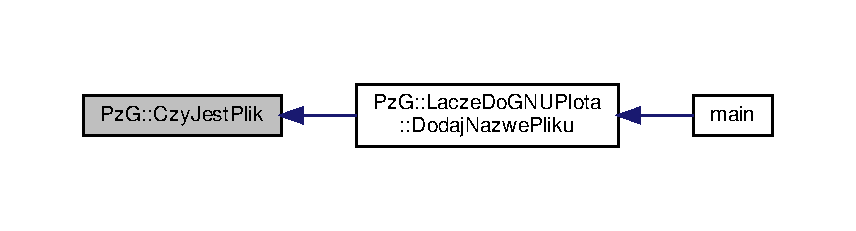
\includegraphics[width=350pt]{namespace_pz_g_ae1ae4d36f66c77879380ba73da8e20e3_icgraph}
\end{center}
\end{figure}

\chapter{Class Documentation}
\hypertarget{class_dron}{}\section{Dron Class Reference}
\label{class_dron}\index{Dron@{Dron}}


Klasa określa współrzędne rotorów oraz korpusu. Jest fragmentem objektu sceny.  




{\ttfamily \#include $<$Dron.\+hh$>$}



Inheritance diagram for Dron\+:
\nopagebreak
\begin{figure}[H]
\begin{center}
\leavevmode
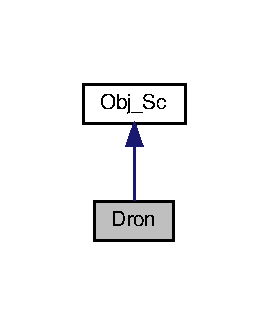
\includegraphics[width=129pt]{class_dron__inherit__graph}
\end{center}
\end{figure}


Collaboration diagram for Dron\+:
\nopagebreak
\begin{figure}[H]
\begin{center}
\leavevmode
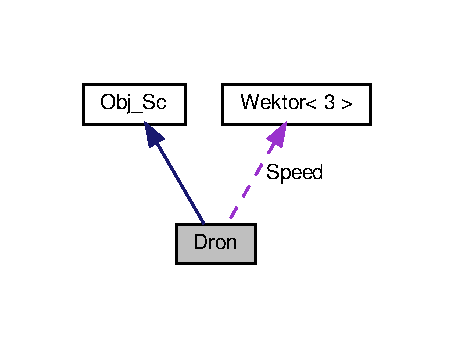
\includegraphics[width=218pt]{class_dron__coll__graph}
\end{center}
\end{figure}
\subsection*{Public Member Functions}
\begin{DoxyCompactItemize}
\item 
double \hyperlink{class_dron_a3d1518d64638aaa98519d240b6455c8c}{Radius} ()
\item 
\hyperlink{_wektor3_d_8hh_ac353a272b38b4ad342f7181ad7bdb91a}{Wektor3D} \hyperlink{class_dron_ae217b4b77f300658ade9817dbc3d0ffa}{Point} ()
\item 
void \hyperlink{class_dron_ae59a8da00fb889c8f97ae08b21a184f9}{Rotate} (int kat)
\item 
void \hyperlink{class_dron_ac9b37f92a345cce27dbc7c16cd40ce27}{Translate} (\hyperlink{_wektor3_d_8hh_ac353a272b38b4ad342f7181ad7bdb91a}{Wektor3D} V)
\item 
\hyperlink{class_prostopadloscian}{Prostopadloscian} \& \hyperlink{class_dron_ad7c1cbee3550365921052076d7345e5f}{DownD} (int ind)
\item 
\hyperlink{class_prostopadloscian}{Prostopadloscian} \& \hyperlink{class_dron_ad6273a0942af9e85cf4fa039b36a1f05}{Corpus1} ()
\item 
\hyperlink{class_prostopadloscian}{Prostopadloscian} \hyperlink{class_dron_accc0e928bc7c9c66c779793fd41a81ee}{Corpus} ()
\item 
\hyperlink{class_rotor}{Rotor} \& \hyperlink{class_dron_a7e22e894b00020b62884cfce45850336}{Take} (int ind)
\item 
\hyperlink{class_rotor}{Rotor} \hyperlink{class_dron_a7ba22c83868cd96769061597d1d0ad25}{operator()} (int ind) const
\item 
\hyperlink{class_rotor}{Rotor} \& \hyperlink{class_dron_a0eb520dc02cf3b2df93d5ce5cf240dbc}{operator()} (int ind)
\end{DoxyCompactItemize}
\subsection*{Public Attributes}
\begin{DoxyCompactItemize}
\item 
\hyperlink{_wektor3_d_8hh_ac353a272b38b4ad342f7181ad7bdb91a}{Wektor3D} \hyperlink{class_dron_af79b620c5f561d94e0e53b8f79bc66c7}{Speed}
\end{DoxyCompactItemize}


\subsection{Detailed Description}
Klasa określa współrzędne rotorów oraz korpusu. Jest fragmentem objektu sceny. 

Definition at line 13 of file Dron.\+hh.



\subsection{Member Function Documentation}
\mbox{\Hypertarget{class_dron_accc0e928bc7c9c66c779793fd41a81ee}\label{class_dron_accc0e928bc7c9c66c779793fd41a81ee}} 
\index{Dron@{Dron}!Corpus@{Corpus}}
\index{Corpus@{Corpus}!Dron@{Dron}}
\subsubsection{\texorpdfstring{Corpus()}{Corpus()}}
{\footnotesize\ttfamily \hyperlink{class_prostopadloscian}{Prostopadloscian} Dron\+::\+Corpus (\begin{DoxyParamCaption}{ }\end{DoxyParamCaption})}



Definition at line 23 of file Dron.\+cpp.

\mbox{\Hypertarget{class_dron_ad6273a0942af9e85cf4fa039b36a1f05}\label{class_dron_ad6273a0942af9e85cf4fa039b36a1f05}} 
\index{Dron@{Dron}!Corpus1@{Corpus1}}
\index{Corpus1@{Corpus1}!Dron@{Dron}}
\subsubsection{\texorpdfstring{Corpus1()}{Corpus1()}}
{\footnotesize\ttfamily \hyperlink{class_prostopadloscian}{Prostopadloscian} \& Dron\+::\+Corpus1 (\begin{DoxyParamCaption}{ }\end{DoxyParamCaption})}



Definition at line 15 of file Dron.\+cpp.

\mbox{\Hypertarget{class_dron_ad7c1cbee3550365921052076d7345e5f}\label{class_dron_ad7c1cbee3550365921052076d7345e5f}} 
\index{Dron@{Dron}!DownD@{DownD}}
\index{DownD@{DownD}!Dron@{Dron}}
\subsubsection{\texorpdfstring{Down\+D()}{DownD()}}
{\footnotesize\ttfamily \hyperlink{class_prostopadloscian}{Prostopadloscian} \& Dron\+::\+DownD (\begin{DoxyParamCaption}\item[{int}]{ind }\end{DoxyParamCaption})}



Definition at line 19 of file Dron.\+cpp.

\mbox{\Hypertarget{class_dron_a7ba22c83868cd96769061597d1d0ad25}\label{class_dron_a7ba22c83868cd96769061597d1d0ad25}} 
\index{Dron@{Dron}!operator()@{operator()}}
\index{operator()@{operator()}!Dron@{Dron}}
\subsubsection{\texorpdfstring{operator()()}{operator()()}\hspace{0.1cm}{\footnotesize\ttfamily [1/2]}}
{\footnotesize\ttfamily \hyperlink{class_rotor}{Rotor} Dron\+::operator() (\begin{DoxyParamCaption}\item[{int}]{ind }\end{DoxyParamCaption}) const\hspace{0.3cm}{\ttfamily [inline]}}



Definition at line 36 of file Dron.\+hh.

\mbox{\Hypertarget{class_dron_a0eb520dc02cf3b2df93d5ce5cf240dbc}\label{class_dron_a0eb520dc02cf3b2df93d5ce5cf240dbc}} 
\index{Dron@{Dron}!operator()@{operator()}}
\index{operator()@{operator()}!Dron@{Dron}}
\subsubsection{\texorpdfstring{operator()()}{operator()()}\hspace{0.1cm}{\footnotesize\ttfamily [2/2]}}
{\footnotesize\ttfamily \hyperlink{class_rotor}{Rotor}\& Dron\+::operator() (\begin{DoxyParamCaption}\item[{int}]{ind }\end{DoxyParamCaption})\hspace{0.3cm}{\ttfamily [inline]}}



Definition at line 37 of file Dron.\+hh.

Here is the call graph for this function\+:
\nopagebreak
\begin{figure}[H]
\begin{center}
\leavevmode
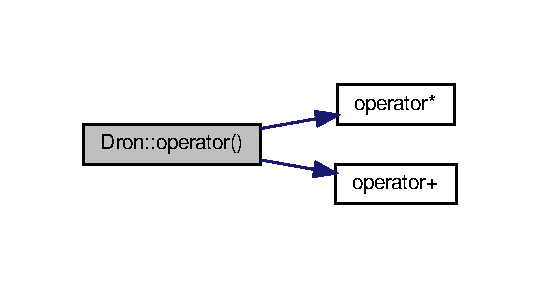
\includegraphics[width=259pt]{class_dron_a0eb520dc02cf3b2df93d5ce5cf240dbc_cgraph}
\end{center}
\end{figure}
\mbox{\Hypertarget{class_dron_ae217b4b77f300658ade9817dbc3d0ffa}\label{class_dron_ae217b4b77f300658ade9817dbc3d0ffa}} 
\index{Dron@{Dron}!Point@{Point}}
\index{Point@{Point}!Dron@{Dron}}
\subsubsection{\texorpdfstring{Point()}{Point()}}
{\footnotesize\ttfamily \hyperlink{_wektor3_d_8hh_ac353a272b38b4ad342f7181ad7bdb91a}{Wektor3D} Dron\+::\+Point (\begin{DoxyParamCaption}{ }\end{DoxyParamCaption})}



Definition at line 10 of file Dron.\+cpp.

\mbox{\Hypertarget{class_dron_a3d1518d64638aaa98519d240b6455c8c}\label{class_dron_a3d1518d64638aaa98519d240b6455c8c}} 
\index{Dron@{Dron}!Radius@{Radius}}
\index{Radius@{Radius}!Dron@{Dron}}
\subsubsection{\texorpdfstring{Radius()}{Radius()}}
{\footnotesize\ttfamily double Dron\+::\+Radius (\begin{DoxyParamCaption}{ }\end{DoxyParamCaption})}



Definition at line 4 of file Dron.\+cpp.

Here is the call graph for this function\+:
\nopagebreak
\begin{figure}[H]
\begin{center}
\leavevmode
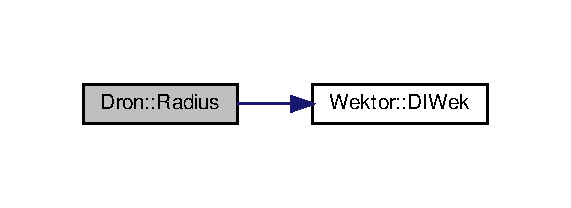
\includegraphics[width=274pt]{class_dron_a3d1518d64638aaa98519d240b6455c8c_cgraph}
\end{center}
\end{figure}
\mbox{\Hypertarget{class_dron_ae59a8da00fb889c8f97ae08b21a184f9}\label{class_dron_ae59a8da00fb889c8f97ae08b21a184f9}} 
\index{Dron@{Dron}!Rotate@{Rotate}}
\index{Rotate@{Rotate}!Dron@{Dron}}
\subsubsection{\texorpdfstring{Rotate()}{Rotate()}}
{\footnotesize\ttfamily void Dron\+::\+Rotate (\begin{DoxyParamCaption}\item[{int}]{kat }\end{DoxyParamCaption})}



Definition at line 27 of file Dron.\+cpp.

Here is the call graph for this function\+:
\nopagebreak
\begin{figure}[H]
\begin{center}
\leavevmode
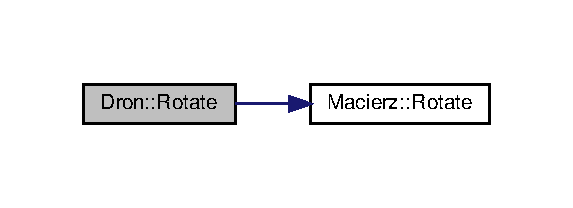
\includegraphics[width=275pt]{class_dron_ae59a8da00fb889c8f97ae08b21a184f9_cgraph}
\end{center}
\end{figure}
\mbox{\Hypertarget{class_dron_a7e22e894b00020b62884cfce45850336}\label{class_dron_a7e22e894b00020b62884cfce45850336}} 
\index{Dron@{Dron}!Take@{Take}}
\index{Take@{Take}!Dron@{Dron}}
\subsubsection{\texorpdfstring{Take()}{Take()}}
{\footnotesize\ttfamily \hyperlink{class_rotor}{Rotor}\& Dron\+::\+Take (\begin{DoxyParamCaption}\item[{int}]{ind }\end{DoxyParamCaption})\hspace{0.3cm}{\ttfamily [inline]}}



Definition at line 33 of file Dron.\+hh.

\mbox{\Hypertarget{class_dron_ac9b37f92a345cce27dbc7c16cd40ce27}\label{class_dron_ac9b37f92a345cce27dbc7c16cd40ce27}} 
\index{Dron@{Dron}!Translate@{Translate}}
\index{Translate@{Translate}!Dron@{Dron}}
\subsubsection{\texorpdfstring{Translate()}{Translate()}}
{\footnotesize\ttfamily void Dron\+::\+Translate (\begin{DoxyParamCaption}\item[{\hyperlink{_wektor3_d_8hh_ac353a272b38b4ad342f7181ad7bdb91a}{Wektor3D}}]{V }\end{DoxyParamCaption})}



Definition at line 56 of file Dron.\+cpp.



\subsection{Member Data Documentation}
\mbox{\Hypertarget{class_dron_af79b620c5f561d94e0e53b8f79bc66c7}\label{class_dron_af79b620c5f561d94e0e53b8f79bc66c7}} 
\index{Dron@{Dron}!Speed@{Speed}}
\index{Speed@{Speed}!Dron@{Dron}}
\subsubsection{\texorpdfstring{Speed}{Speed}}
{\footnotesize\ttfamily \hyperlink{_wektor3_d_8hh_ac353a272b38b4ad342f7181ad7bdb91a}{Wektor3D} Dron\+::\+Speed}



Definition at line 24 of file Dron.\+hh.



The documentation for this class was generated from the following files\+:\begin{DoxyCompactItemize}
\item 
inc/\hyperlink{_dron_8hh}{Dron.\+hh}\item 
src/\hyperlink{_dron_8cpp}{Dron.\+cpp}\end{DoxyCompactItemize}

\hypertarget{class_pz_g_1_1_info_pliku_do_rysowania}{}\section{PzG\+:\+:Info\+Pliku\+Do\+Rysowania Class Reference}
\label{class_pz_g_1_1_info_pliku_do_rysowania}\index{Pz\+G\+::\+Info\+Pliku\+Do\+Rysowania@{Pz\+G\+::\+Info\+Pliku\+Do\+Rysowania}}


Zestaw informacji dotyczący pliku i sposobu rysowania.  




{\ttfamily \#include $<$lacze\+\_\+do\+\_\+gnuplota.\+hh$>$}

\subsection*{Public Member Functions}
\begin{DoxyCompactItemize}
\item 
\hyperlink{class_pz_g_1_1_info_pliku_do_rysowania_a48bc8ad94ef5fd5120b668a566c9172e}{Info\+Pliku\+Do\+Rysowania} (const char $\ast$Nazwa\+Pliku, \hyperlink{namespace_pz_g_a705c92106f39b7d0c34a6739d10ff0b6}{Rodzaj\+Rysowania} Rodz\+Rys, int Szerokosc)
\item 
const std\+::string \hyperlink{class_pz_g_1_1_info_pliku_do_rysowania_ac92a5dc258f9b6164631e2ea5247a7a7}{Wez\+Nazwe\+Pliku} () const
\begin{DoxyCompactList}\small\item\em Udostępia nazwę pliku do rysowania. \end{DoxyCompactList}\item 
void \hyperlink{class_pz_g_1_1_info_pliku_do_rysowania_ae734c69f5cecf9c0584e3a7f433340ea}{Zmien\+Nazwe\+Pliku} (const std\+::string \&Nazwa\+Pliku)
\begin{DoxyCompactList}\small\item\em Zmienia nazwę pliku do rysowania. \end{DoxyCompactList}\item 
\hyperlink{namespace_pz_g_a705c92106f39b7d0c34a6739d10ff0b6}{Rodzaj\+Rysowania} \hyperlink{class_pz_g_1_1_info_pliku_do_rysowania_a6a46f3c7b7a08dfa9d694f387f873234}{Wez\+Rodz\+Rys} () const
\begin{DoxyCompactList}\small\item\em Udostępnia sposób rysowanej linii. \end{DoxyCompactList}\item 
int \hyperlink{class_pz_g_1_1_info_pliku_do_rysowania_a627bb615c50f3b03374774e6b974488b}{Wez\+Szerokosc} () const
\begin{DoxyCompactList}\small\item\em Udostępnia informację o szerokości linii. \end{DoxyCompactList}\end{DoxyCompactItemize}


\subsection{Detailed Description}
Zestaw informacji dotyczący pliku i sposobu rysowania. 

Klasa modeluje zestaw informacji dotyczący pliku i sposobu w jaki mają być wizualizowane zawarte w nim dane. 

Definition at line 56 of file lacze\+\_\+do\+\_\+gnuplota.\+hh.



\subsection{Constructor \& Destructor Documentation}
\mbox{\Hypertarget{class_pz_g_1_1_info_pliku_do_rysowania_a48bc8ad94ef5fd5120b668a566c9172e}\label{class_pz_g_1_1_info_pliku_do_rysowania_a48bc8ad94ef5fd5120b668a566c9172e}} 
\index{Pz\+G\+::\+Info\+Pliku\+Do\+Rysowania@{Pz\+G\+::\+Info\+Pliku\+Do\+Rysowania}!Info\+Pliku\+Do\+Rysowania@{Info\+Pliku\+Do\+Rysowania}}
\index{Info\+Pliku\+Do\+Rysowania@{Info\+Pliku\+Do\+Rysowania}!Pz\+G\+::\+Info\+Pliku\+Do\+Rysowania@{Pz\+G\+::\+Info\+Pliku\+Do\+Rysowania}}
\subsubsection{\texorpdfstring{Info\+Pliku\+Do\+Rysowania()}{InfoPlikuDoRysowania()}}
{\footnotesize\ttfamily Pz\+G\+::\+Info\+Pliku\+Do\+Rysowania\+::\+Info\+Pliku\+Do\+Rysowania (\begin{DoxyParamCaption}\item[{const char $\ast$}]{Nazwa\+Pliku,  }\item[{\hyperlink{namespace_pz_g_a705c92106f39b7d0c34a6739d10ff0b6}{Rodzaj\+Rysowania}}]{Rodz\+Rys,  }\item[{int}]{Szerokosc }\end{DoxyParamCaption})\hspace{0.3cm}{\ttfamily [inline]}}

Inicjalizuje obiekt. 
\begin{DoxyParams}{Parameters}
{\em Nazwa\+Pliku} & -\/ nazwa pliku, z którego pobierane będą dane, \\
\hline
{\em Rodz\+Rys} & -\/ rodzaj rysowania linii, \\
\hline
{\em Szerokosc} & -\/ szerokosc linii. \\
\hline
\end{DoxyParams}


Definition at line 64 of file lacze\+\_\+do\+\_\+gnuplota.\+hh.



\subsection{Member Function Documentation}
\mbox{\Hypertarget{class_pz_g_1_1_info_pliku_do_rysowania_ac92a5dc258f9b6164631e2ea5247a7a7}\label{class_pz_g_1_1_info_pliku_do_rysowania_ac92a5dc258f9b6164631e2ea5247a7a7}} 
\index{Pz\+G\+::\+Info\+Pliku\+Do\+Rysowania@{Pz\+G\+::\+Info\+Pliku\+Do\+Rysowania}!Wez\+Nazwe\+Pliku@{Wez\+Nazwe\+Pliku}}
\index{Wez\+Nazwe\+Pliku@{Wez\+Nazwe\+Pliku}!Pz\+G\+::\+Info\+Pliku\+Do\+Rysowania@{Pz\+G\+::\+Info\+Pliku\+Do\+Rysowania}}
\subsubsection{\texorpdfstring{Wez\+Nazwe\+Pliku()}{WezNazwePliku()}}
{\footnotesize\ttfamily const std\+::string Pz\+G\+::\+Info\+Pliku\+Do\+Rysowania\+::\+Wez\+Nazwe\+Pliku (\begin{DoxyParamCaption}{ }\end{DoxyParamCaption}) const\hspace{0.3cm}{\ttfamily [inline]}}



Udostępia nazwę pliku do rysowania. 

Udostępnia nazwę pliku z danymi do rysowania. 

Definition at line 75 of file lacze\+\_\+do\+\_\+gnuplota.\+hh.

\mbox{\Hypertarget{class_pz_g_1_1_info_pliku_do_rysowania_a6a46f3c7b7a08dfa9d694f387f873234}\label{class_pz_g_1_1_info_pliku_do_rysowania_a6a46f3c7b7a08dfa9d694f387f873234}} 
\index{Pz\+G\+::\+Info\+Pliku\+Do\+Rysowania@{Pz\+G\+::\+Info\+Pliku\+Do\+Rysowania}!Wez\+Rodz\+Rys@{Wez\+Rodz\+Rys}}
\index{Wez\+Rodz\+Rys@{Wez\+Rodz\+Rys}!Pz\+G\+::\+Info\+Pliku\+Do\+Rysowania@{Pz\+G\+::\+Info\+Pliku\+Do\+Rysowania}}
\subsubsection{\texorpdfstring{Wez\+Rodz\+Rys()}{WezRodzRys()}}
{\footnotesize\ttfamily \hyperlink{namespace_pz_g_a705c92106f39b7d0c34a6739d10ff0b6}{Rodzaj\+Rysowania} Pz\+G\+::\+Info\+Pliku\+Do\+Rysowania\+::\+Wez\+Rodz\+Rys (\begin{DoxyParamCaption}{ }\end{DoxyParamCaption}) const\hspace{0.3cm}{\ttfamily [inline]}}



Udostępnia sposób rysowanej linii. 

Udostępnia informację o sposóbie rysowania linii. 

Definition at line 87 of file lacze\+\_\+do\+\_\+gnuplota.\+hh.

\mbox{\Hypertarget{class_pz_g_1_1_info_pliku_do_rysowania_a627bb615c50f3b03374774e6b974488b}\label{class_pz_g_1_1_info_pliku_do_rysowania_a627bb615c50f3b03374774e6b974488b}} 
\index{Pz\+G\+::\+Info\+Pliku\+Do\+Rysowania@{Pz\+G\+::\+Info\+Pliku\+Do\+Rysowania}!Wez\+Szerokosc@{Wez\+Szerokosc}}
\index{Wez\+Szerokosc@{Wez\+Szerokosc}!Pz\+G\+::\+Info\+Pliku\+Do\+Rysowania@{Pz\+G\+::\+Info\+Pliku\+Do\+Rysowania}}
\subsubsection{\texorpdfstring{Wez\+Szerokosc()}{WezSzerokosc()}}
{\footnotesize\ttfamily int Pz\+G\+::\+Info\+Pliku\+Do\+Rysowania\+::\+Wez\+Szerokosc (\begin{DoxyParamCaption}{ }\end{DoxyParamCaption}) const\hspace{0.3cm}{\ttfamily [inline]}}



Udostępnia informację o szerokości linii. 

Udostępnia informację o szerokości rysowanej linii. 

Definition at line 93 of file lacze\+\_\+do\+\_\+gnuplota.\+hh.

\mbox{\Hypertarget{class_pz_g_1_1_info_pliku_do_rysowania_ae734c69f5cecf9c0584e3a7f433340ea}\label{class_pz_g_1_1_info_pliku_do_rysowania_ae734c69f5cecf9c0584e3a7f433340ea}} 
\index{Pz\+G\+::\+Info\+Pliku\+Do\+Rysowania@{Pz\+G\+::\+Info\+Pliku\+Do\+Rysowania}!Zmien\+Nazwe\+Pliku@{Zmien\+Nazwe\+Pliku}}
\index{Zmien\+Nazwe\+Pliku@{Zmien\+Nazwe\+Pliku}!Pz\+G\+::\+Info\+Pliku\+Do\+Rysowania@{Pz\+G\+::\+Info\+Pliku\+Do\+Rysowania}}
\subsubsection{\texorpdfstring{Zmien\+Nazwe\+Pliku()}{ZmienNazwePliku()}}
{\footnotesize\ttfamily void Pz\+G\+::\+Info\+Pliku\+Do\+Rysowania\+::\+Zmien\+Nazwe\+Pliku (\begin{DoxyParamCaption}\item[{const std\+::string \&}]{Nazwa\+Pliku }\end{DoxyParamCaption})\hspace{0.3cm}{\ttfamily [inline]}}



Zmienia nazwę pliku do rysowania. 

Zmienia nazwę pliku z danymi do rysowania. 

Definition at line 81 of file lacze\+\_\+do\+\_\+gnuplota.\+hh.



The documentation for this class was generated from the following file\+:\begin{DoxyCompactItemize}
\item 
inc/\hyperlink{lacze__do__gnuplota_8hh}{lacze\+\_\+do\+\_\+gnuplota.\+hh}\end{DoxyCompactItemize}

\hypertarget{class_pz_g_1_1_lacze_do_g_n_u_plota}{}\section{PzG\+:\+:Lacze\+Do\+G\+N\+U\+Plota Class Reference}
\label{class_pz_g_1_1_lacze_do_g_n_u_plota}\index{Pz\+G\+::\+Lacze\+Do\+G\+N\+U\+Plota@{Pz\+G\+::\+Lacze\+Do\+G\+N\+U\+Plota}}


Klasa realizuje interfejs do programu G\+N\+U\+Plot.  




{\ttfamily \#include $<$lacze\+\_\+do\+\_\+gnuplota.\+hh$>$}

\subsection*{Public Member Functions}
\begin{DoxyCompactItemize}
\item 
void \hyperlink{class_pz_g_1_1_lacze_do_g_n_u_plota_a11421d7c67deab6b7524cc492407e897}{Pokaz\+Os\+\_\+\+OX} (bool Pokaz)
\begin{DoxyCompactList}\small\item\em Umożliwia lub zabrania rysowania osi OX. \end{DoxyCompactList}\item 
bool \hyperlink{class_pz_g_1_1_lacze_do_g_n_u_plota_ae112972af57167c3b053bf922bce6bbf}{Pokaz\+Os\+\_\+\+OX} () const
\begin{DoxyCompactList}\small\item\em Czy oś OX ma być rysowana. \end{DoxyCompactList}\item 
void \hyperlink{class_pz_g_1_1_lacze_do_g_n_u_plota_a7c3db909b266fc30808e86406c04b516}{Pokaz\+Os\+\_\+\+OY} (bool Pokaz)
\begin{DoxyCompactList}\small\item\em Umożliwia lub zabrania rysowania osi OY. \end{DoxyCompactList}\item 
bool \hyperlink{class_pz_g_1_1_lacze_do_g_n_u_plota_a7298f469f6932f5c808dcf620650b4b8}{Pokaz\+Os\+\_\+\+OY} () const
\begin{DoxyCompactList}\small\item\em Czy oś OY ma być rysowana. \end{DoxyCompactList}\item 
void \hyperlink{class_pz_g_1_1_lacze_do_g_n_u_plota_a9fabfe88cb1801a5de8923f45f514b99}{Pokaz\+Os\+\_\+\+OZ} (bool Pokaz)
\begin{DoxyCompactList}\small\item\em Umożliwia lub zabrania rysowania osi OZ. \end{DoxyCompactList}\item 
bool \hyperlink{class_pz_g_1_1_lacze_do_g_n_u_plota_a22c708af33c57bf3b5d1b4e82b4017b7}{Pokaz\+Os\+\_\+\+OZ} () const
\begin{DoxyCompactList}\small\item\em Czy oś OZ ma być rysowana. \end{DoxyCompactList}\item 
float \hyperlink{class_pz_g_1_1_lacze_do_g_n_u_plota_a66836c9749bf179420e4ca3e9447efd7}{Xmin} () const
\item 
float \hyperlink{class_pz_g_1_1_lacze_do_g_n_u_plota_a8e23479629af3df3d352b7839ae396b8}{Xmax} () const
\item 
float \hyperlink{class_pz_g_1_1_lacze_do_g_n_u_plota_a9352c0382bfaeaaba9f65399a7383164}{Ymin} () const
\item 
float \hyperlink{class_pz_g_1_1_lacze_do_g_n_u_plota_ac54e4e7448ce3bd324efdc94a999f535}{Ymax} () const
\item 
float \hyperlink{class_pz_g_1_1_lacze_do_g_n_u_plota_a9068bd9a9873ba9c6d70016f1ae7cd7f}{Zmin} () const
\item 
float \hyperlink{class_pz_g_1_1_lacze_do_g_n_u_plota_a20a5d03e1fc19c682032bffc54340f12}{Zmax} () const
\item 
void \hyperlink{class_pz_g_1_1_lacze_do_g_n_u_plota_a10950349b348fd3a3d4143e95337527c}{Zmien\+Tryb\+Rys} (\hyperlink{namespace_pz_g_aeedae1ef10c66d720f9e89de408ca4ca}{Tryb\+Rysowania} Tryb)
\begin{DoxyCompactList}\small\item\em Zmienia tryb rysowania. \end{DoxyCompactList}\item 
\hyperlink{namespace_pz_g_aeedae1ef10c66d720f9e89de408ca4ca}{Tryb\+Rysowania} \hyperlink{class_pz_g_1_1_lacze_do_g_n_u_plota_a7c417f27b4b112f58a5be3ce6ea8d1fe}{Wez\+Tryb\+Rys} () const
\begin{DoxyCompactList}\small\item\em Udostępnia aktualny tryb rysowania. \end{DoxyCompactList}\item 
void \hyperlink{class_pz_g_1_1_lacze_do_g_n_u_plota_a9c91987dfc869d6fcea96205c581daef}{Ustaw\+ZakresX} (float Xo, float Xn)
\begin{DoxyCompactList}\small\item\em Ustawia zakres osi {\itshape OX}. \end{DoxyCompactList}\item 
void \hyperlink{class_pz_g_1_1_lacze_do_g_n_u_plota_a54c6e9cf9ab2eae479451fd953c2717c}{Ustaw\+ZakresY} (float Yo, float Yn)
\begin{DoxyCompactList}\small\item\em Ustawia zakres osi {\itshape OY}. \end{DoxyCompactList}\item 
void \hyperlink{class_pz_g_1_1_lacze_do_g_n_u_plota_a1dbbb2b86fb13b8632e6bad9df2a82e3}{Ustaw\+ZakresZ} (float Zo, float Zn)
\begin{DoxyCompactList}\small\item\em Ustawia zakres osi {\itshape OZ}. \end{DoxyCompactList}\item 
float \hyperlink{class_pz_g_1_1_lacze_do_g_n_u_plota_a4b1eb252fd785a5aeff938e7b2dce2b1}{SkalaX} () const
\begin{DoxyCompactList}\small\item\em Udostępnia skalę dla osi {\itshape OX}. \end{DoxyCompactList}\item 
float \hyperlink{class_pz_g_1_1_lacze_do_g_n_u_plota_a44f922ccbc508d6cd7809c669238dae3}{SkalaZ} () const
\begin{DoxyCompactList}\small\item\em Udostępnia skalę dla osi {\itshape OZ}. \end{DoxyCompactList}\item 
void \hyperlink{class_pz_g_1_1_lacze_do_g_n_u_plota_a855b8338bfe3e5d294d719f24b11090e}{Ustaw\+SkaleX} (float skala\+\_\+x)
\begin{DoxyCompactList}\small\item\em Zadaje skalę wzdłuż osi {\itshape OZ}. \end{DoxyCompactList}\item 
void \hyperlink{class_pz_g_1_1_lacze_do_g_n_u_plota_ab0486db3166d8db6580a221079af241f}{Ustaw\+SkaleZ} (float skala\+\_\+z)
\begin{DoxyCompactList}\small\item\em Zadaje skalę wzdłuż osi {\itshape OZ}. \end{DoxyCompactList}\item 
void \hyperlink{class_pz_g_1_1_lacze_do_g_n_u_plota_a4308151b54e105d302803146a3238699}{Ustaw\+Skale\+XZ} (float skala\+\_\+x, float skala\+\_\+z)
\begin{DoxyCompactList}\small\item\em Zadaje skalę wzdłuż osi {\itshape OX} i {\itshape OZ}. \end{DoxyCompactList}\item 
float \hyperlink{class_pz_g_1_1_lacze_do_g_n_u_plota_addf0b844f626f3f5220de70efcbbdbb3}{RotacjaX} () const
\item 
float \hyperlink{class_pz_g_1_1_lacze_do_g_n_u_plota_a9dac73754fab10644b287756003e9c79}{RotacjaZ} () const
\item 
void \hyperlink{class_pz_g_1_1_lacze_do_g_n_u_plota_a88324c53a70846fb6bc9d918ce21fd56}{Ustaw\+RotacjeX} (float kat\+\_\+x)
\begin{DoxyCompactList}\small\item\em Ustawia rotację wokół osi {\itshape OX}. \end{DoxyCompactList}\item 
void \hyperlink{class_pz_g_1_1_lacze_do_g_n_u_plota_a458399aa2a8f4b3f00ccd5b272857ea1}{Ustaw\+RotacjeZ} (float kat\+\_\+z)
\begin{DoxyCompactList}\small\item\em Ustawia rotację wokół osi {\itshape OZ}. \end{DoxyCompactList}\item 
void \hyperlink{class_pz_g_1_1_lacze_do_g_n_u_plota_a94d8527fd78048ed6cb32ffb29e5f903}{Ustaw\+Rotacje\+XZ} (float kat\+\_\+x, float kat\+\_\+z)
\begin{DoxyCompactList}\small\item\em Ustawia rotację wokół osi {\itshape OX} i {\itshape OZ}. \end{DoxyCompactList}\item 
void \hyperlink{class_pz_g_1_1_lacze_do_g_n_u_plota_a4531e6d166faf2e2c8bb4a54a9c9e1f8}{Wyswietlaj\+Komunikaty\+Bledow} (bool Tryb=true)
\begin{DoxyCompactList}\small\item\em Zezwala lub zabrania wyświetlania komunikatów. \end{DoxyCompactList}\item 
bool \hyperlink{class_pz_g_1_1_lacze_do_g_n_u_plota_a34bd48f57c0fd69c12bf4127a1cacd8f}{Dodaj\+Nazwe\+Pliku} (const char $\ast$Nazwa\+Pliku, \hyperlink{namespace_pz_g_a705c92106f39b7d0c34a6739d10ff0b6}{Rodzaj\+Rysowania} Rodz\+Rys=\hyperlink{namespace_pz_g_a705c92106f39b7d0c34a6739d10ff0b6a927eaa159aa4bd3198f0a330b967746d}{R\+R\+\_\+\+Ciagly}, int Szerokosc=1)
\begin{DoxyCompactList}\small\item\em Dodaje nazwę pliku. \end{DoxyCompactList}\item 
bool \hyperlink{class_pz_g_1_1_lacze_do_g_n_u_plota_ad3d7607946b82aa941d786dcd086d27e}{Dopisz\+Rysowanie\+Z\+Plikow} (std\+::string \&Polecenie, char const $\ast$$\ast$Sep)
\begin{DoxyCompactList}\small\item\em Tworzy listę parametrów umożliwiających rysowanie brył z plików. \end{DoxyCompactList}\item 
bool \hyperlink{class_pz_g_1_1_lacze_do_g_n_u_plota_af8be8aeb3b1b524fab67d4411cba5b9e}{Czy\+Polaczenie\+Jest\+Zainicjowane} () const
\begin{DoxyCompactList}\small\item\em Informuje, czy połączenie z {\itshape gnuplot\textquotesingle{}em} jest zainicjalizowane. \end{DoxyCompactList}\item 
bool \hyperlink{class_pz_g_1_1_lacze_do_g_n_u_plota_a065f5b8402737cc62b0ad4f66d028335}{Rysuj} ()
\item 
bool \hyperlink{class_pz_g_1_1_lacze_do_g_n_u_plota_addae9ac156ae2fb227f792faff3aa148}{Rysuj\+Do\+Pliku} (const char $\ast$Nazwa\+Pliku)
\item 
bool \hyperlink{class_pz_g_1_1_lacze_do_g_n_u_plota_a200ce6bdb980c314a9eafe49e8f2dd5e}{Inicjalizuj} ()
\begin{DoxyCompactList}\small\item\em Inicjalizuje połączenie z programem {\itshape gnuplot}. \end{DoxyCompactList}\item 
void \hyperlink{class_pz_g_1_1_lacze_do_g_n_u_plota_a75f599f17413ea8602c6dbba09f36407}{Usun\+Ostatnia\+Nazwe} ()
\begin{DoxyCompactList}\small\item\em Usuwa ostatnią nazwę pliku. \end{DoxyCompactList}\item 
void \hyperlink{class_pz_g_1_1_lacze_do_g_n_u_plota_a89a1d90d017d264cd26398464d074073}{Usun\+Wszystkie\+Nazwy\+Plikow} ()
\begin{DoxyCompactList}\small\item\em Kasuje zawartość listy nazw plików. \end{DoxyCompactList}\item 
\hyperlink{class_pz_g_1_1_lacze_do_g_n_u_plota_a5845189b5ab8c3634acf57024e5deeaf}{Lacze\+Do\+G\+N\+U\+Plota} ()
\item 
virtual \hyperlink{class_pz_g_1_1_lacze_do_g_n_u_plota_afc10ec7f193032ecae714f6d832dcbf0}{$\sim$\+Lacze\+Do\+G\+N\+U\+Plota} ()
\end{DoxyCompactItemize}
\subsection*{Protected Member Functions}
\begin{DoxyCompactItemize}
\item 
virtual bool \hyperlink{class_pz_g_1_1_lacze_do_g_n_u_plota_a25585ec3f1bd3b6bf42f374c38b8d237}{Dopisz\+Pliki\+Do\+Polecenia\+Rysowania} (std\+::string \&Polecenie, char const $\ast$$\ast$Sep)
\begin{DoxyCompactList}\small\item\em Tworzy listę parametrów umożliwiających rysowanie dodatkowych elementów. \end{DoxyCompactList}\item 
std\+::string \hyperlink{class_pz_g_1_1_lacze_do_g_n_u_plota_a4579aecf7b4777fdde0cae4e98c275c2}{Zapisz\+Ustawienie\+Zakresu} (char Os) const
\begin{DoxyCompactList}\small\item\em Tworzy polecenie ustawiające zakres dla danej współrzędnej. \end{DoxyCompactList}\item 
std\+::string \hyperlink{class_pz_g_1_1_lacze_do_g_n_u_plota_aa92b463e8cbae31b50dd797a4183bce8}{Zapisz\+Ustawienie\+Rotacji\+I\+Skali} () const
\begin{DoxyCompactList}\small\item\em Tworzy polecenie ustawiające punkt obserwacji. \end{DoxyCompactList}\item 
bool \hyperlink{class_pz_g_1_1_lacze_do_g_n_u_plota_a5063854b7232a7951d120a21df63f2b7}{Przeslij\+Do\+G\+N\+U\+Plota} (const char $\ast$Polecenie)
\item 
bool \hyperlink{class_pz_g_1_1_lacze_do_g_n_u_plota_a5e4f3a226ed36f7110032d802d84847c}{Czy\+Wyswietlac\+Komunikaty} () const
\begin{DoxyCompactList}\small\item\em Udostępnia informację czy mają być wyświetlane informacje o błędach. \end{DoxyCompactList}\item 
bool \hyperlink{class_pz_g_1_1_lacze_do_g_n_u_plota_a1c7b9acc40de8d8bbb40fb0722512933}{Utworz\+Proces\+Potomny} ()
\begin{DoxyCompactList}\small\item\em Uruchamia program {\itshape gnuplot} jako proces potomny. \end{DoxyCompactList}\item 
void \hyperlink{class_pz_g_1_1_lacze_do_g_n_u_plota_a90056743aeaa546721528005f2cf41e6}{Komunikat\+Bledu} (const char $\ast$Komunikat) const
\item 
void \hyperlink{class_pz_g_1_1_lacze_do_g_n_u_plota_a0da98f68f533070d5a32adbdb519cf56}{Buduj\+Preambule\+Polecenia\+Rysowania} (std\+::string \&Preambula) const
\begin{DoxyCompactList}\small\item\em Tworzy preambułę poprzedzającą polecenie rysowania. \end{DoxyCompactList}\item 
void \hyperlink{class_pz_g_1_1_lacze_do_g_n_u_plota_a0ac655ff1934abb69ea668cd92ae77ec}{Buduj\+Preambule\+\_\+2D} (std\+::string \&Preambula) const
\begin{DoxyCompactList}\small\item\em Tworzy preambułę poprzedzającą polecenie rysowania w trybie 2D. \end{DoxyCompactList}\item 
void \hyperlink{class_pz_g_1_1_lacze_do_g_n_u_plota_a50a544677e52829cac4dd4a95b821dcb}{Buduj\+Preambule\+\_\+3D} (std\+::string \&Preambula) const
\begin{DoxyCompactList}\small\item\em Tworzy preambułę poprzedzającą polecenie rysowania w trybie 3D. \end{DoxyCompactList}\end{DoxyCompactItemize}
\subsection*{Protected Attributes}
\begin{DoxyCompactItemize}
\item 
int \hyperlink{class_pz_g_1_1_lacze_do_g_n_u_plota_adc3a2250216c2473a61da379da70b2d7}{\+\_\+\+Wejscie\+\_\+\+G\+N\+U\+Plota}
\item 
int \hyperlink{class_pz_g_1_1_lacze_do_g_n_u_plota_a7d05a4767a35ee494d59724bb740dbc2}{\+\_\+\+Wyjscie\+\_\+\+G\+N\+U\+Plota}
\item 
bool \hyperlink{class_pz_g_1_1_lacze_do_g_n_u_plota_a2f2800f14ebfe1caef0b4d30c410a7fe}{\+\_\+\+Wyswietlaj\+Komunikaty\+O\+Bledach}
\begin{DoxyCompactList}\small\item\em Decyduje czy mają być wyświetlane komunikaty o błędach, czy też nie. \end{DoxyCompactList}\item 
\hyperlink{namespace_pz_g_aeedae1ef10c66d720f9e89de408ca4ca}{Tryb\+Rysowania} \hyperlink{class_pz_g_1_1_lacze_do_g_n_u_plota_a00e3a51bb47d3fb26eee875dc48215db}{\+\_\+\+Tryb\+Rys}
\begin{DoxyCompactList}\small\item\em Określa aktualny tryb rysowania. \end{DoxyCompactList}\item 
float \hyperlink{class_pz_g_1_1_lacze_do_g_n_u_plota_a69d530edfe769e38448972e897456deb}{\+\_\+\+Xmin}
\begin{DoxyCompactList}\small\item\em Dolny zakres wyświetlanej skali skali dla osi {\itshape OX}. \end{DoxyCompactList}\item 
float \hyperlink{class_pz_g_1_1_lacze_do_g_n_u_plota_a847e00678a413ab076ccbcb7eba3ae58}{\+\_\+\+Xmax}
\begin{DoxyCompactList}\small\item\em Górny zakres wyświetlanej skali skali dla osi {\itshape OX}. \end{DoxyCompactList}\item 
float \hyperlink{class_pz_g_1_1_lacze_do_g_n_u_plota_abc555fd6b82b0d5c9efb4802b58dc317}{\+\_\+\+Ymin}
\begin{DoxyCompactList}\small\item\em Dolny zakres wyświetlanej skali skali dla osi {\itshape OY}. \end{DoxyCompactList}\item 
float \hyperlink{class_pz_g_1_1_lacze_do_g_n_u_plota_ad7dfd3fad82ea0720ec89eacc18410bf}{\+\_\+\+Ymax}
\begin{DoxyCompactList}\small\item\em Górny zakres wyświetlanej skali skali dla osi {\itshape OY}. \end{DoxyCompactList}\item 
float \hyperlink{class_pz_g_1_1_lacze_do_g_n_u_plota_a8f9797e881df35f4206cb7d8030e5edc}{\+\_\+\+Zmin}
\begin{DoxyCompactList}\small\item\em Dolny zakres wyświetlanej skali skali dla osi {\itshape OZ}. \end{DoxyCompactList}\item 
float \hyperlink{class_pz_g_1_1_lacze_do_g_n_u_plota_a26949eedd421832f0f206ce3c8f90694}{\+\_\+\+Zmax}
\begin{DoxyCompactList}\small\item\em Górny zakres wyświetlanej skali skali dla osi {\itshape OZ}. \end{DoxyCompactList}\item 
float \hyperlink{class_pz_g_1_1_lacze_do_g_n_u_plota_a2c9303c4dbb4c9f0ddc4f1fe02eb3f70}{\+\_\+\+Xskala}
\item 
float \hyperlink{class_pz_g_1_1_lacze_do_g_n_u_plota_a85446d06b2d714b2f852ef43c47c73c1}{\+\_\+\+Zskala}
\item 
float \hyperlink{class_pz_g_1_1_lacze_do_g_n_u_plota_a21e77f0a2bfb7fed989b6dc2d64b5a7e}{\+\_\+\+Xrotacja}
\item 
float \hyperlink{class_pz_g_1_1_lacze_do_g_n_u_plota_aa65781b1ff96dfb31a780e98ee28d6ed}{\+\_\+\+Zrotacja}
\item 
bool \hyperlink{class_pz_g_1_1_lacze_do_g_n_u_plota_a833aa8994b9913786f920ec8c259731f}{\+\_\+\+Pokaz\+Os\+\_\+\+OX}
\begin{DoxyCompactList}\small\item\em Czy oś OX ma być widoczna. \end{DoxyCompactList}\item 
bool \hyperlink{class_pz_g_1_1_lacze_do_g_n_u_plota_ae8d9b4dac5eae6ce86b7043c45b70ed8}{\+\_\+\+Pokaz\+Os\+\_\+\+OY}
\begin{DoxyCompactList}\small\item\em Czy oś OY ma być widoczna. \end{DoxyCompactList}\item 
bool \hyperlink{class_pz_g_1_1_lacze_do_g_n_u_plota_a5b0afc06dc248790d2e7475b2162e309}{\+\_\+\+Pokaz\+Os\+\_\+\+OZ}
\begin{DoxyCompactList}\small\item\em Czy oś OZ ma być widoczna. \end{DoxyCompactList}\end{DoxyCompactItemize}
\subsection*{Static Protected Attributes}
\begin{DoxyCompactItemize}
\item 
static std\+::list$<$ \hyperlink{class_pz_g_1_1_info_pliku_do_rysowania}{Info\+Pliku\+Do\+Rysowania} $>$ \hyperlink{class_pz_g_1_1_lacze_do_g_n_u_plota_a1916c5a6fecfb3554e9d5204b2f2086c}{\+\_\+\+Info\+Plikow}
\begin{DoxyCompactList}\small\item\em Lista nazw plików z danymi dla {\itshape gnuplota}. \end{DoxyCompactList}\end{DoxyCompactItemize}


\subsection{Detailed Description}
Klasa realizuje interfejs do programu G\+N\+U\+Plot. 

Klasa realizuje interfejs do programu G\+N\+U\+Plot. Pozwala ona na wskazanie zbioru punktów płaszczyzn umieszczonych w pliku lub plikach. Każdy taki zbiór może być następnie wizualizowany przez program gnuplot w postaci oddzielnych płaszczyzn z wycinaniem części zasłanianych. 

Definition at line 126 of file lacze\+\_\+do\+\_\+gnuplota.\+hh.



\subsection{Constructor \& Destructor Documentation}
\mbox{\Hypertarget{class_pz_g_1_1_lacze_do_g_n_u_plota_a5845189b5ab8c3634acf57024e5deeaf}\label{class_pz_g_1_1_lacze_do_g_n_u_plota_a5845189b5ab8c3634acf57024e5deeaf}} 
\index{Pz\+G\+::\+Lacze\+Do\+G\+N\+U\+Plota@{Pz\+G\+::\+Lacze\+Do\+G\+N\+U\+Plota}!Lacze\+Do\+G\+N\+U\+Plota@{Lacze\+Do\+G\+N\+U\+Plota}}
\index{Lacze\+Do\+G\+N\+U\+Plota@{Lacze\+Do\+G\+N\+U\+Plota}!Pz\+G\+::\+Lacze\+Do\+G\+N\+U\+Plota@{Pz\+G\+::\+Lacze\+Do\+G\+N\+U\+Plota}}
\subsubsection{\texorpdfstring{Lacze\+Do\+G\+N\+U\+Plota()}{LaczeDoGNUPlota()}}
{\footnotesize\ttfamily Pz\+G\+::\+Lacze\+Do\+G\+N\+U\+Plota\+::\+Lacze\+Do\+G\+N\+U\+Plota (\begin{DoxyParamCaption}{ }\end{DoxyParamCaption})}



Definition at line 59 of file lacze\+\_\+do\+\_\+gnuplota.\+cpp.

\mbox{\Hypertarget{class_pz_g_1_1_lacze_do_g_n_u_plota_afc10ec7f193032ecae714f6d832dcbf0}\label{class_pz_g_1_1_lacze_do_g_n_u_plota_afc10ec7f193032ecae714f6d832dcbf0}} 
\index{Pz\+G\+::\+Lacze\+Do\+G\+N\+U\+Plota@{Pz\+G\+::\+Lacze\+Do\+G\+N\+U\+Plota}!````~Lacze\+Do\+G\+N\+U\+Plota@{$\sim$\+Lacze\+Do\+G\+N\+U\+Plota}}
\index{````~Lacze\+Do\+G\+N\+U\+Plota@{$\sim$\+Lacze\+Do\+G\+N\+U\+Plota}!Pz\+G\+::\+Lacze\+Do\+G\+N\+U\+Plota@{Pz\+G\+::\+Lacze\+Do\+G\+N\+U\+Plota}}
\subsubsection{\texorpdfstring{$\sim$\+Lacze\+Do\+G\+N\+U\+Plota()}{~LaczeDoGNUPlota()}}
{\footnotesize\ttfamily Pz\+G\+::\+Lacze\+Do\+G\+N\+U\+Plota\+::$\sim$\+Lacze\+Do\+G\+N\+U\+Plota (\begin{DoxyParamCaption}{ }\end{DoxyParamCaption})\hspace{0.3cm}{\ttfamily [virtual]}}



Definition at line 35 of file lacze\+\_\+do\+\_\+gnuplota.\+cpp.



\subsection{Member Function Documentation}
\mbox{\Hypertarget{class_pz_g_1_1_lacze_do_g_n_u_plota_a0ac655ff1934abb69ea668cd92ae77ec}\label{class_pz_g_1_1_lacze_do_g_n_u_plota_a0ac655ff1934abb69ea668cd92ae77ec}} 
\index{Pz\+G\+::\+Lacze\+Do\+G\+N\+U\+Plota@{Pz\+G\+::\+Lacze\+Do\+G\+N\+U\+Plota}!Buduj\+Preambule\+\_\+2D@{Buduj\+Preambule\+\_\+2D}}
\index{Buduj\+Preambule\+\_\+2D@{Buduj\+Preambule\+\_\+2D}!Pz\+G\+::\+Lacze\+Do\+G\+N\+U\+Plota@{Pz\+G\+::\+Lacze\+Do\+G\+N\+U\+Plota}}
\subsubsection{\texorpdfstring{Buduj\+Preambule\+\_\+2\+D()}{BudujPreambule\_2D()}}
{\footnotesize\ttfamily void Pz\+G\+::\+Lacze\+Do\+G\+N\+U\+Plota\+::\+Buduj\+Preambule\+\_\+2D (\begin{DoxyParamCaption}\item[{std\+::string \&}]{Preambula }\end{DoxyParamCaption}) const\hspace{0.3cm}{\ttfamily [protected]}}



Tworzy preambułę poprzedzającą polecenie rysowania w trybie 2D. 

Tworzy zbiór poleceń, które ustawiają właściwy tryb rysowania oraz zakresy współrzędnych, jak też wszystkie inne parametry wynikające z trybu rysowania 2D. 

Definition at line 365 of file lacze\+\_\+do\+\_\+gnuplota.\+cpp.

\mbox{\Hypertarget{class_pz_g_1_1_lacze_do_g_n_u_plota_a50a544677e52829cac4dd4a95b821dcb}\label{class_pz_g_1_1_lacze_do_g_n_u_plota_a50a544677e52829cac4dd4a95b821dcb}} 
\index{Pz\+G\+::\+Lacze\+Do\+G\+N\+U\+Plota@{Pz\+G\+::\+Lacze\+Do\+G\+N\+U\+Plota}!Buduj\+Preambule\+\_\+3D@{Buduj\+Preambule\+\_\+3D}}
\index{Buduj\+Preambule\+\_\+3D@{Buduj\+Preambule\+\_\+3D}!Pz\+G\+::\+Lacze\+Do\+G\+N\+U\+Plota@{Pz\+G\+::\+Lacze\+Do\+G\+N\+U\+Plota}}
\subsubsection{\texorpdfstring{Buduj\+Preambule\+\_\+3\+D()}{BudujPreambule\_3D()}}
{\footnotesize\ttfamily void Pz\+G\+::\+Lacze\+Do\+G\+N\+U\+Plota\+::\+Buduj\+Preambule\+\_\+3D (\begin{DoxyParamCaption}\item[{std\+::string \&}]{Preambula }\end{DoxyParamCaption}) const\hspace{0.3cm}{\ttfamily [protected]}}



Tworzy preambułę poprzedzającą polecenie rysowania w trybie 3D. 

Tworzy zbiór poleceń, które ustawiają właściwy tryb rysowania oraz zakresy współrzędnych, jak też wszystkie inne parametry wynikające z trybu rysowania 3D. 

Definition at line 381 of file lacze\+\_\+do\+\_\+gnuplota.\+cpp.

\mbox{\Hypertarget{class_pz_g_1_1_lacze_do_g_n_u_plota_a0da98f68f533070d5a32adbdb519cf56}\label{class_pz_g_1_1_lacze_do_g_n_u_plota_a0da98f68f533070d5a32adbdb519cf56}} 
\index{Pz\+G\+::\+Lacze\+Do\+G\+N\+U\+Plota@{Pz\+G\+::\+Lacze\+Do\+G\+N\+U\+Plota}!Buduj\+Preambule\+Polecenia\+Rysowania@{Buduj\+Preambule\+Polecenia\+Rysowania}}
\index{Buduj\+Preambule\+Polecenia\+Rysowania@{Buduj\+Preambule\+Polecenia\+Rysowania}!Pz\+G\+::\+Lacze\+Do\+G\+N\+U\+Plota@{Pz\+G\+::\+Lacze\+Do\+G\+N\+U\+Plota}}
\subsubsection{\texorpdfstring{Buduj\+Preambule\+Polecenia\+Rysowania()}{BudujPreambulePoleceniaRysowania()}}
{\footnotesize\ttfamily void Pz\+G\+::\+Lacze\+Do\+G\+N\+U\+Plota\+::\+Buduj\+Preambule\+Polecenia\+Rysowania (\begin{DoxyParamCaption}\item[{std\+::string \&}]{Preambula }\end{DoxyParamCaption}) const\hspace{0.3cm}{\ttfamily [protected]}}



Tworzy preambułę poprzedzającą polecenie rysowania. 

Tworzy zbiór poleceń, które ustawiają właściwy tryb rysowania oraz zakresy współrzędnych, jak też wszystkie inne parametry wynikające z przyjętego trybu rysowania. 

Definition at line 355 of file lacze\+\_\+do\+\_\+gnuplota.\+cpp.

\mbox{\Hypertarget{class_pz_g_1_1_lacze_do_g_n_u_plota_af8be8aeb3b1b524fab67d4411cba5b9e}\label{class_pz_g_1_1_lacze_do_g_n_u_plota_af8be8aeb3b1b524fab67d4411cba5b9e}} 
\index{Pz\+G\+::\+Lacze\+Do\+G\+N\+U\+Plota@{Pz\+G\+::\+Lacze\+Do\+G\+N\+U\+Plota}!Czy\+Polaczenie\+Jest\+Zainicjowane@{Czy\+Polaczenie\+Jest\+Zainicjowane}}
\index{Czy\+Polaczenie\+Jest\+Zainicjowane@{Czy\+Polaczenie\+Jest\+Zainicjowane}!Pz\+G\+::\+Lacze\+Do\+G\+N\+U\+Plota@{Pz\+G\+::\+Lacze\+Do\+G\+N\+U\+Plota}}
\subsubsection{\texorpdfstring{Czy\+Polaczenie\+Jest\+Zainicjowane()}{CzyPolaczenieJestZainicjowane()}}
{\footnotesize\ttfamily bool Pz\+G\+::\+Lacze\+Do\+G\+N\+U\+Plota\+::\+Czy\+Polaczenie\+Jest\+Zainicjowane (\begin{DoxyParamCaption}{ }\end{DoxyParamCaption}) const}



Informuje, czy połączenie z {\itshape gnuplot\textquotesingle{}em} jest zainicjalizowane. 

Informuje, czy połączenie z programem {\itshape gnuplot} jest zainicjowane. 
\begin{DoxyRetVals}{Return values}
{\em true} & -\/ jeśli tak, \\
\hline
{\em false} & -\/ w przypadku przeciwnym. \\
\hline
\end{DoxyRetVals}


Definition at line 124 of file lacze\+\_\+do\+\_\+gnuplota.\+cpp.

\mbox{\Hypertarget{class_pz_g_1_1_lacze_do_g_n_u_plota_a5e4f3a226ed36f7110032d802d84847c}\label{class_pz_g_1_1_lacze_do_g_n_u_plota_a5e4f3a226ed36f7110032d802d84847c}} 
\index{Pz\+G\+::\+Lacze\+Do\+G\+N\+U\+Plota@{Pz\+G\+::\+Lacze\+Do\+G\+N\+U\+Plota}!Czy\+Wyswietlac\+Komunikaty@{Czy\+Wyswietlac\+Komunikaty}}
\index{Czy\+Wyswietlac\+Komunikaty@{Czy\+Wyswietlac\+Komunikaty}!Pz\+G\+::\+Lacze\+Do\+G\+N\+U\+Plota@{Pz\+G\+::\+Lacze\+Do\+G\+N\+U\+Plota}}
\subsubsection{\texorpdfstring{Czy\+Wyswietlac\+Komunikaty()}{CzyWyswietlacKomunikaty()}}
{\footnotesize\ttfamily bool Pz\+G\+::\+Lacze\+Do\+G\+N\+U\+Plota\+::\+Czy\+Wyswietlac\+Komunikaty (\begin{DoxyParamCaption}{ }\end{DoxyParamCaption}) const\hspace{0.3cm}{\ttfamily [inline]}, {\ttfamily [protected]}}



Udostępnia informację czy mają być wyświetlane informacje o błędach. 

Udostępnia wartość pola \hyperlink{class_pz_g_1_1_lacze_do_g_n_u_plota_a2f2800f14ebfe1caef0b4d30c410a7fe}{\+\_\+\+Wyswietlaj\+Komunikaty\+O\+Bledach}. Określa ono, czy mają być wyświetlane komunikaty o błędach na wyjście standardowe, czy też nie. 

Definition at line 308 of file lacze\+\_\+do\+\_\+gnuplota.\+hh.

\mbox{\Hypertarget{class_pz_g_1_1_lacze_do_g_n_u_plota_a34bd48f57c0fd69c12bf4127a1cacd8f}\label{class_pz_g_1_1_lacze_do_g_n_u_plota_a34bd48f57c0fd69c12bf4127a1cacd8f}} 
\index{Pz\+G\+::\+Lacze\+Do\+G\+N\+U\+Plota@{Pz\+G\+::\+Lacze\+Do\+G\+N\+U\+Plota}!Dodaj\+Nazwe\+Pliku@{Dodaj\+Nazwe\+Pliku}}
\index{Dodaj\+Nazwe\+Pliku@{Dodaj\+Nazwe\+Pliku}!Pz\+G\+::\+Lacze\+Do\+G\+N\+U\+Plota@{Pz\+G\+::\+Lacze\+Do\+G\+N\+U\+Plota}}
\subsubsection{\texorpdfstring{Dodaj\+Nazwe\+Pliku()}{DodajNazwePliku()}}
{\footnotesize\ttfamily bool Pz\+G\+::\+Lacze\+Do\+G\+N\+U\+Plota\+::\+Dodaj\+Nazwe\+Pliku (\begin{DoxyParamCaption}\item[{const char $\ast$}]{Nazwa\+Pliku,  }\item[{\hyperlink{namespace_pz_g_a705c92106f39b7d0c34a6739d10ff0b6}{Rodzaj\+Rysowania}}]{Rodz\+Rys = {\ttfamily \hyperlink{namespace_pz_g_a705c92106f39b7d0c34a6739d10ff0b6a927eaa159aa4bd3198f0a330b967746d}{R\+R\+\_\+\+Ciagly}},  }\item[{int}]{Szerokosc = {\ttfamily 1} }\end{DoxyParamCaption})}



Dodaje nazwę pliku. 

Powoduje dodanie do listy plików zawierajacych dane dla {\itshape gnuplota}, nowej nazwy pliku.


\begin{DoxyParams}[1]{Parameters}
\mbox{\tt in}  & {\em Nazwa\+Pliku} & -\/ nazwa pliku z danymi dla gnuplota. \\
\hline
\mbox{\tt in}  & {\em Rodz\+Rys} & -\/ tryb rysowania danego zbioru punktow. Może być ciągły lub jako zbiór osobnych punktów. \\
\hline
\mbox{\tt in}  & {\em Szerokosc} & -\/ szerokość rysowanego obiektu. W przypadku punktów parametr ten jest połową szerokości kwadratu reprezentującego dany punkt.\\
\hline
\end{DoxyParams}

\begin{DoxyRetVals}{Return values}
{\em true} & -\/ jeżeli istnieje plik o nazwie udostępnionej poprzez parametr {\itshape Nazwa\+Pliku} oraz jest zezwolenie na jego czytanie. Nazwa pliku zostaje dodana do listy plików z danymi dla {\itshape gnuplota}. \\
\hline
{\em false} & -\/ Jeżeli nie istnieje plik o nazwie przekazanej poprzez parametr {\itshape Nazwa\+Pliku}. Nazwa pliku zostaje dodana do listy plików z danymi dla {\itshape gnuplota}. \\
\hline
\end{DoxyRetVals}


Definition at line 102 of file lacze\+\_\+do\+\_\+gnuplota.\+cpp.

Here is the call graph for this function\+:\nopagebreak
\begin{figure}[H]
\begin{center}
\leavevmode
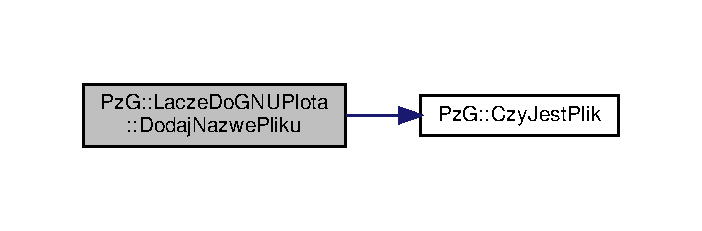
\includegraphics[width=337pt]{class_pz_g_1_1_lacze_do_g_n_u_plota_a34bd48f57c0fd69c12bf4127a1cacd8f_cgraph}
\end{center}
\end{figure}
Here is the caller graph for this function\+:\nopagebreak
\begin{figure}[H]
\begin{center}
\leavevmode
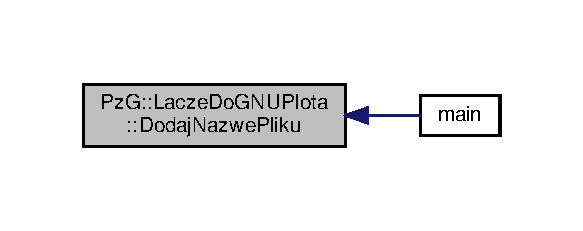
\includegraphics[width=280pt]{class_pz_g_1_1_lacze_do_g_n_u_plota_a34bd48f57c0fd69c12bf4127a1cacd8f_icgraph}
\end{center}
\end{figure}
\mbox{\Hypertarget{class_pz_g_1_1_lacze_do_g_n_u_plota_a25585ec3f1bd3b6bf42f374c38b8d237}\label{class_pz_g_1_1_lacze_do_g_n_u_plota_a25585ec3f1bd3b6bf42f374c38b8d237}} 
\index{Pz\+G\+::\+Lacze\+Do\+G\+N\+U\+Plota@{Pz\+G\+::\+Lacze\+Do\+G\+N\+U\+Plota}!Dopisz\+Pliki\+Do\+Polecenia\+Rysowania@{Dopisz\+Pliki\+Do\+Polecenia\+Rysowania}}
\index{Dopisz\+Pliki\+Do\+Polecenia\+Rysowania@{Dopisz\+Pliki\+Do\+Polecenia\+Rysowania}!Pz\+G\+::\+Lacze\+Do\+G\+N\+U\+Plota@{Pz\+G\+::\+Lacze\+Do\+G\+N\+U\+Plota}}
\subsubsection{\texorpdfstring{Dopisz\+Pliki\+Do\+Polecenia\+Rysowania()}{DopiszPlikiDoPoleceniaRysowania()}}
{\footnotesize\ttfamily bool Pz\+G\+::\+Lacze\+Do\+G\+N\+U\+Plota\+::\+Dopisz\+Pliki\+Do\+Polecenia\+Rysowania (\begin{DoxyParamCaption}\item[{std\+::string \&}]{Polecenie,  }\item[{char const $\ast$$\ast$}]{Sep }\end{DoxyParamCaption})\hspace{0.3cm}{\ttfamily [inline]}, {\ttfamily [protected]}, {\ttfamily [virtual]}}



Tworzy listę parametrów umożliwiających rysowanie dodatkowych elementów. 

Metoda ta przewidziana jest jako element rozszerzenia pozwalającego w klasach pochodnych powiększyć listę rysowanych elementów. \begin{DoxyPrecond}{Precondition}
Parametr {\itshape Polecenie} powinien zawierać polecenie {\itshape plot} lub {\itshape splot}, do którego będzie możliwe dopisanie dalszego ciągu. 
\end{DoxyPrecond}

\begin{DoxyParams}{Parameters}
{\em Polecenie} & -\/ polecenie rysowania, do którego mają być dopisane nazwy plików i odpowiednie parametry dla polecenia plot. \\
\hline
{\em Sep} & -\/ zawiera znak separatora między poszczególnymi parametrami. Jeżeli parametry listy przeszkód są generowane jako pierwsze, to zmienna ta musi być wskaźnikiem do wskaźnika na łańcuch\+: \char`\"{} \char`\"{}. \\
\hline
\end{DoxyParams}


Definition at line 690 of file lacze\+\_\+do\+\_\+gnuplota.\+hh.

\mbox{\Hypertarget{class_pz_g_1_1_lacze_do_g_n_u_plota_ad3d7607946b82aa941d786dcd086d27e}\label{class_pz_g_1_1_lacze_do_g_n_u_plota_ad3d7607946b82aa941d786dcd086d27e}} 
\index{Pz\+G\+::\+Lacze\+Do\+G\+N\+U\+Plota@{Pz\+G\+::\+Lacze\+Do\+G\+N\+U\+Plota}!Dopisz\+Rysowanie\+Z\+Plikow@{Dopisz\+Rysowanie\+Z\+Plikow}}
\index{Dopisz\+Rysowanie\+Z\+Plikow@{Dopisz\+Rysowanie\+Z\+Plikow}!Pz\+G\+::\+Lacze\+Do\+G\+N\+U\+Plota@{Pz\+G\+::\+Lacze\+Do\+G\+N\+U\+Plota}}
\subsubsection{\texorpdfstring{Dopisz\+Rysowanie\+Z\+Plikow()}{DopiszRysowanieZPlikow()}}
{\footnotesize\ttfamily bool Pz\+G\+::\+Lacze\+Do\+G\+N\+U\+Plota\+::\+Dopisz\+Rysowanie\+Z\+Plikow (\begin{DoxyParamCaption}\item[{std\+::string \&}]{Polecenie,  }\item[{char const $\ast$$\ast$}]{Sep }\end{DoxyParamCaption})}



Tworzy listę parametrów umożliwiających rysowanie brył z plików. 

Tworzy napis będący parametrami dla polecenie {\itshape plot} programu, {\itshape gnuplot}. Parametry te pozwalają na rysowanie brył, których współrzędne wierzchołków zawarte są w plikach. Nazwy tych plików muszą być wcześniej dołączone do kolejki plików poprzez zastosowanie polecenia \hyperlink{}{Dodaj\+Nazwe}.


\begin{DoxyParams}{Parameters}
{\em Polecenie} & -\/ dopisywana jest do niego sekwencja znaków tworzących parametry dla polecenia {\itshape plot}. \\
\hline
{\em Sep} & -\/ zawiera znak separatora między poszczególnymi parametrami. Jeżeli parametry listy nazw plików są generowane jako pierwsze, to zmienna ta musi być wskaźnikiem do wskaźnika na łańcuch\+: \char`\"{} \char`\"{}. \\
\hline
\end{DoxyParams}

\begin{DoxyRetVals}{Return values}
{\em true} & -\/ jeśli lista nazw plików nie jest pusta. \\
\hline
{\em false} & -\/ w przypadku przeciwnym. \\
\hline
\end{DoxyRetVals}
\begin{DoxyPostcond}{Postcondition}
Jeżeli lista nazw plików nie jest pusta, to poprzez parametr {\itshape Sep} zostaje udostępniony łańcuch\+: \char`\"{}, \char`\"{}. 
\end{DoxyPostcond}


Definition at line 287 of file lacze\+\_\+do\+\_\+gnuplota.\+cpp.

\mbox{\Hypertarget{class_pz_g_1_1_lacze_do_g_n_u_plota_a200ce6bdb980c314a9eafe49e8f2dd5e}\label{class_pz_g_1_1_lacze_do_g_n_u_plota_a200ce6bdb980c314a9eafe49e8f2dd5e}} 
\index{Pz\+G\+::\+Lacze\+Do\+G\+N\+U\+Plota@{Pz\+G\+::\+Lacze\+Do\+G\+N\+U\+Plota}!Inicjalizuj@{Inicjalizuj}}
\index{Inicjalizuj@{Inicjalizuj}!Pz\+G\+::\+Lacze\+Do\+G\+N\+U\+Plota@{Pz\+G\+::\+Lacze\+Do\+G\+N\+U\+Plota}}
\subsubsection{\texorpdfstring{Inicjalizuj()}{Inicjalizuj()}}
{\footnotesize\ttfamily bool Pz\+G\+::\+Lacze\+Do\+G\+N\+U\+Plota\+::\+Inicjalizuj (\begin{DoxyParamCaption}{ }\end{DoxyParamCaption})}



Inicjalizuje połączenie z programem {\itshape gnuplot}. 

Inicjalizuje połączenie z programem {\itshape gnuplot}. Realizowane jest to poprzez rozwidlenie procesu i uruchomienie jako procesu potomnego programu {\itshape gnuplot}. Komunikacja z programem {\itshape gnuplot} realizowana jest poprzez przejęcie jego wejścia i wyjścia standardowego.


\begin{DoxyRetVals}{Return values}
{\em true} & -\/ gdy połączenie z programem {\itshape 0gnuplot} zostało poprawnie zainicjalizowane lub gdy już wcześniej było zainicjalizowane. \\
\hline
{\em false} & -\/ gdy proces inicjalizacji połączenia zakończył się niepowodzeniem. \\
\hline
\end{DoxyRetVals}


Definition at line 141 of file lacze\+\_\+do\+\_\+gnuplota.\+cpp.

\mbox{\Hypertarget{class_pz_g_1_1_lacze_do_g_n_u_plota_a90056743aeaa546721528005f2cf41e6}\label{class_pz_g_1_1_lacze_do_g_n_u_plota_a90056743aeaa546721528005f2cf41e6}} 
\index{Pz\+G\+::\+Lacze\+Do\+G\+N\+U\+Plota@{Pz\+G\+::\+Lacze\+Do\+G\+N\+U\+Plota}!Komunikat\+Bledu@{Komunikat\+Bledu}}
\index{Komunikat\+Bledu@{Komunikat\+Bledu}!Pz\+G\+::\+Lacze\+Do\+G\+N\+U\+Plota@{Pz\+G\+::\+Lacze\+Do\+G\+N\+U\+Plota}}
\subsubsection{\texorpdfstring{Komunikat\+Bledu()}{KomunikatBledu()}}
{\footnotesize\ttfamily void Pz\+G\+::\+Lacze\+Do\+G\+N\+U\+Plota\+::\+Komunikat\+Bledu (\begin{DoxyParamCaption}\item[{const char $\ast$}]{Komunikat }\end{DoxyParamCaption}) const\hspace{0.3cm}{\ttfamily [protected]}}

Wyświetla na wyjście \char`\"{}standard error\char`\"{} komunikat (przekazany jako parametr), o ile pole \hyperlink{class_pz_g_1_1_lacze_do_g_n_u_plota_a2f2800f14ebfe1caef0b4d30c410a7fe}{\+\_\+\+Wyswietlaj\+Komunikaty\+O\+Bledach} ma wartość {\ttfamily true}. W przypadku przeciwnym komunikat nie jest wyświetlany. 

Definition at line 130 of file lacze\+\_\+do\+\_\+gnuplota.\+cpp.

\mbox{\Hypertarget{class_pz_g_1_1_lacze_do_g_n_u_plota_a11421d7c67deab6b7524cc492407e897}\label{class_pz_g_1_1_lacze_do_g_n_u_plota_a11421d7c67deab6b7524cc492407e897}} 
\index{Pz\+G\+::\+Lacze\+Do\+G\+N\+U\+Plota@{Pz\+G\+::\+Lacze\+Do\+G\+N\+U\+Plota}!Pokaz\+Os\+\_\+\+OX@{Pokaz\+Os\+\_\+\+OX}}
\index{Pokaz\+Os\+\_\+\+OX@{Pokaz\+Os\+\_\+\+OX}!Pz\+G\+::\+Lacze\+Do\+G\+N\+U\+Plota@{Pz\+G\+::\+Lacze\+Do\+G\+N\+U\+Plota}}
\subsubsection{\texorpdfstring{Pokaz\+Os\+\_\+\+O\+X()}{PokazOs\_OX()}\hspace{0.1cm}{\footnotesize\ttfamily [1/2]}}
{\footnotesize\ttfamily void Pz\+G\+::\+Lacze\+Do\+G\+N\+U\+Plota\+::\+Pokaz\+Os\+\_\+\+OX (\begin{DoxyParamCaption}\item[{bool}]{Pokaz }\end{DoxyParamCaption})\hspace{0.3cm}{\ttfamily [inline]}}



Umożliwia lub zabrania rysowania osi OX. 

Umożliwia lub zabrania rysowania osi {\itshape OX} na rysunku wykresu. 
\begin{DoxyParams}{Parameters}
{\em Pokaz} & -\/ decyduje o tym czy oś {\itshape OX} będzie rysowana ({\ttfamily true}), czy też nie ({\ttfamily false}). \\
\hline
\end{DoxyParams}


Definition at line 360 of file lacze\+\_\+do\+\_\+gnuplota.\+hh.

\mbox{\Hypertarget{class_pz_g_1_1_lacze_do_g_n_u_plota_ae112972af57167c3b053bf922bce6bbf}\label{class_pz_g_1_1_lacze_do_g_n_u_plota_ae112972af57167c3b053bf922bce6bbf}} 
\index{Pz\+G\+::\+Lacze\+Do\+G\+N\+U\+Plota@{Pz\+G\+::\+Lacze\+Do\+G\+N\+U\+Plota}!Pokaz\+Os\+\_\+\+OX@{Pokaz\+Os\+\_\+\+OX}}
\index{Pokaz\+Os\+\_\+\+OX@{Pokaz\+Os\+\_\+\+OX}!Pz\+G\+::\+Lacze\+Do\+G\+N\+U\+Plota@{Pz\+G\+::\+Lacze\+Do\+G\+N\+U\+Plota}}
\subsubsection{\texorpdfstring{Pokaz\+Os\+\_\+\+O\+X()}{PokazOs\_OX()}\hspace{0.1cm}{\footnotesize\ttfamily [2/2]}}
{\footnotesize\ttfamily bool Pz\+G\+::\+Lacze\+Do\+G\+N\+U\+Plota\+::\+Pokaz\+Os\+\_\+\+OX (\begin{DoxyParamCaption}{ }\end{DoxyParamCaption}) const\hspace{0.3cm}{\ttfamily [inline]}}



Czy oś OX ma być rysowana. 

Udostępnia informację czy oś {\itshape OX} ma być rysowana, czy też nie. 
\begin{DoxyRetVals}{Return values}
{\em true} & -\/ gdy oś {\itshape OX} ma być rysowana, \\
\hline
{\em false} & -\/ w przypadku przeciwnym. \\
\hline
\end{DoxyRetVals}


Definition at line 370 of file lacze\+\_\+do\+\_\+gnuplota.\+hh.

\mbox{\Hypertarget{class_pz_g_1_1_lacze_do_g_n_u_plota_a7c3db909b266fc30808e86406c04b516}\label{class_pz_g_1_1_lacze_do_g_n_u_plota_a7c3db909b266fc30808e86406c04b516}} 
\index{Pz\+G\+::\+Lacze\+Do\+G\+N\+U\+Plota@{Pz\+G\+::\+Lacze\+Do\+G\+N\+U\+Plota}!Pokaz\+Os\+\_\+\+OY@{Pokaz\+Os\+\_\+\+OY}}
\index{Pokaz\+Os\+\_\+\+OY@{Pokaz\+Os\+\_\+\+OY}!Pz\+G\+::\+Lacze\+Do\+G\+N\+U\+Plota@{Pz\+G\+::\+Lacze\+Do\+G\+N\+U\+Plota}}
\subsubsection{\texorpdfstring{Pokaz\+Os\+\_\+\+O\+Y()}{PokazOs\_OY()}\hspace{0.1cm}{\footnotesize\ttfamily [1/2]}}
{\footnotesize\ttfamily void Pz\+G\+::\+Lacze\+Do\+G\+N\+U\+Plota\+::\+Pokaz\+Os\+\_\+\+OY (\begin{DoxyParamCaption}\item[{bool}]{Pokaz }\end{DoxyParamCaption})\hspace{0.3cm}{\ttfamily [inline]}}



Umożliwia lub zabrania rysowania osi OY. 

Umożliwia lub zabrania rysowania osi {\itshape OY} na rysunku wykresu. 
\begin{DoxyParams}{Parameters}
{\em Pokaz} & -\/ decyduje o tym czy oś {\itshape OY} będzie rysowana ({\ttfamily true}), czy też nie ({\ttfamily false}). \\
\hline
\end{DoxyParams}


Definition at line 380 of file lacze\+\_\+do\+\_\+gnuplota.\+hh.

\mbox{\Hypertarget{class_pz_g_1_1_lacze_do_g_n_u_plota_a7298f469f6932f5c808dcf620650b4b8}\label{class_pz_g_1_1_lacze_do_g_n_u_plota_a7298f469f6932f5c808dcf620650b4b8}} 
\index{Pz\+G\+::\+Lacze\+Do\+G\+N\+U\+Plota@{Pz\+G\+::\+Lacze\+Do\+G\+N\+U\+Plota}!Pokaz\+Os\+\_\+\+OY@{Pokaz\+Os\+\_\+\+OY}}
\index{Pokaz\+Os\+\_\+\+OY@{Pokaz\+Os\+\_\+\+OY}!Pz\+G\+::\+Lacze\+Do\+G\+N\+U\+Plota@{Pz\+G\+::\+Lacze\+Do\+G\+N\+U\+Plota}}
\subsubsection{\texorpdfstring{Pokaz\+Os\+\_\+\+O\+Y()}{PokazOs\_OY()}\hspace{0.1cm}{\footnotesize\ttfamily [2/2]}}
{\footnotesize\ttfamily bool Pz\+G\+::\+Lacze\+Do\+G\+N\+U\+Plota\+::\+Pokaz\+Os\+\_\+\+OY (\begin{DoxyParamCaption}{ }\end{DoxyParamCaption}) const\hspace{0.3cm}{\ttfamily [inline]}}



Czy oś OY ma być rysowana. 

Udostępnia informację czy oś {\itshape OY} ma być rysowana, czy też nie. 
\begin{DoxyRetVals}{Return values}
{\em true} & -\/ gdy oś {\itshape OY} ma być rysowana, \\
\hline
{\em false} & -\/ w przypadku przeciwnym. \\
\hline
\end{DoxyRetVals}


Definition at line 390 of file lacze\+\_\+do\+\_\+gnuplota.\+hh.

\mbox{\Hypertarget{class_pz_g_1_1_lacze_do_g_n_u_plota_a9fabfe88cb1801a5de8923f45f514b99}\label{class_pz_g_1_1_lacze_do_g_n_u_plota_a9fabfe88cb1801a5de8923f45f514b99}} 
\index{Pz\+G\+::\+Lacze\+Do\+G\+N\+U\+Plota@{Pz\+G\+::\+Lacze\+Do\+G\+N\+U\+Plota}!Pokaz\+Os\+\_\+\+OZ@{Pokaz\+Os\+\_\+\+OZ}}
\index{Pokaz\+Os\+\_\+\+OZ@{Pokaz\+Os\+\_\+\+OZ}!Pz\+G\+::\+Lacze\+Do\+G\+N\+U\+Plota@{Pz\+G\+::\+Lacze\+Do\+G\+N\+U\+Plota}}
\subsubsection{\texorpdfstring{Pokaz\+Os\+\_\+\+O\+Z()}{PokazOs\_OZ()}\hspace{0.1cm}{\footnotesize\ttfamily [1/2]}}
{\footnotesize\ttfamily void Pz\+G\+::\+Lacze\+Do\+G\+N\+U\+Plota\+::\+Pokaz\+Os\+\_\+\+OZ (\begin{DoxyParamCaption}\item[{bool}]{Pokaz }\end{DoxyParamCaption})\hspace{0.3cm}{\ttfamily [inline]}}



Umożliwia lub zabrania rysowania osi OZ. 

Umożliwia lub zabrania rysowania osi {\itshape OZ} na rysunku wykresu. 
\begin{DoxyParams}{Parameters}
{\em Pokaz} & -\/ decyduje o tym czy oś {\itshape OZ} będzie rysowana ({\ttfamily true}), czy też nie ({\ttfamily false}). \\
\hline
\end{DoxyParams}


Definition at line 400 of file lacze\+\_\+do\+\_\+gnuplota.\+hh.

\mbox{\Hypertarget{class_pz_g_1_1_lacze_do_g_n_u_plota_a22c708af33c57bf3b5d1b4e82b4017b7}\label{class_pz_g_1_1_lacze_do_g_n_u_plota_a22c708af33c57bf3b5d1b4e82b4017b7}} 
\index{Pz\+G\+::\+Lacze\+Do\+G\+N\+U\+Plota@{Pz\+G\+::\+Lacze\+Do\+G\+N\+U\+Plota}!Pokaz\+Os\+\_\+\+OZ@{Pokaz\+Os\+\_\+\+OZ}}
\index{Pokaz\+Os\+\_\+\+OZ@{Pokaz\+Os\+\_\+\+OZ}!Pz\+G\+::\+Lacze\+Do\+G\+N\+U\+Plota@{Pz\+G\+::\+Lacze\+Do\+G\+N\+U\+Plota}}
\subsubsection{\texorpdfstring{Pokaz\+Os\+\_\+\+O\+Z()}{PokazOs\_OZ()}\hspace{0.1cm}{\footnotesize\ttfamily [2/2]}}
{\footnotesize\ttfamily bool Pz\+G\+::\+Lacze\+Do\+G\+N\+U\+Plota\+::\+Pokaz\+Os\+\_\+\+OZ (\begin{DoxyParamCaption}{ }\end{DoxyParamCaption}) const\hspace{0.3cm}{\ttfamily [inline]}}



Czy oś OZ ma być rysowana. 

Udostępnia informację czy oś {\itshape OZ} ma być rysowana, czy też nie. 
\begin{DoxyRetVals}{Return values}
{\em true} & -\/ gdy oś {\itshape OZ} ma być rysowana, \\
\hline
{\em false} & -\/ w przypadku przeciwnym. \\
\hline
\end{DoxyRetVals}


Definition at line 410 of file lacze\+\_\+do\+\_\+gnuplota.\+hh.

\mbox{\Hypertarget{class_pz_g_1_1_lacze_do_g_n_u_plota_a5063854b7232a7951d120a21df63f2b7}\label{class_pz_g_1_1_lacze_do_g_n_u_plota_a5063854b7232a7951d120a21df63f2b7}} 
\index{Pz\+G\+::\+Lacze\+Do\+G\+N\+U\+Plota@{Pz\+G\+::\+Lacze\+Do\+G\+N\+U\+Plota}!Przeslij\+Do\+G\+N\+U\+Plota@{Przeslij\+Do\+G\+N\+U\+Plota}}
\index{Przeslij\+Do\+G\+N\+U\+Plota@{Przeslij\+Do\+G\+N\+U\+Plota}!Pz\+G\+::\+Lacze\+Do\+G\+N\+U\+Plota@{Pz\+G\+::\+Lacze\+Do\+G\+N\+U\+Plota}}
\subsubsection{\texorpdfstring{Przeslij\+Do\+G\+N\+U\+Plota()}{PrzeslijDoGNUPlota()}}
{\footnotesize\ttfamily bool Pz\+G\+::\+Lacze\+Do\+G\+N\+U\+Plota\+::\+Przeslij\+Do\+G\+N\+U\+Plota (\begin{DoxyParamCaption}\item[{const char $\ast$}]{Polecenie }\end{DoxyParamCaption})\hspace{0.3cm}{\ttfamily [protected]}}

Przesyła na wejście programu {\itshape gnuplot} zadany ciąg znaków. 
\begin{DoxyParams}{Parameters}
{\em Polecenie} & -\/ komunikat przeznaczony do przeslania.\\
\hline
\end{DoxyParams}
\begin{DoxyPrecond}{Precondition}
Musi być zainicjowane połączenie z programem gnuplot.
\end{DoxyPrecond}

\begin{DoxyRetVals}{Return values}
{\em true} & -\/ jesli przeslanie polecenia zakończyło się powodzeniem, \\
\hline
{\em false} & -\/ w przypadku przeciwnym. \\
\hline
\end{DoxyRetVals}


Definition at line 39 of file lacze\+\_\+do\+\_\+gnuplota.\+cpp.

\mbox{\Hypertarget{class_pz_g_1_1_lacze_do_g_n_u_plota_addf0b844f626f3f5220de70efcbbdbb3}\label{class_pz_g_1_1_lacze_do_g_n_u_plota_addf0b844f626f3f5220de70efcbbdbb3}} 
\index{Pz\+G\+::\+Lacze\+Do\+G\+N\+U\+Plota@{Pz\+G\+::\+Lacze\+Do\+G\+N\+U\+Plota}!RotacjaX@{RotacjaX}}
\index{RotacjaX@{RotacjaX}!Pz\+G\+::\+Lacze\+Do\+G\+N\+U\+Plota@{Pz\+G\+::\+Lacze\+Do\+G\+N\+U\+Plota}}
\subsubsection{\texorpdfstring{Rotacja\+X()}{RotacjaX()}}
{\footnotesize\ttfamily float Pz\+G\+::\+Lacze\+Do\+G\+N\+U\+Plota\+::\+RotacjaX (\begin{DoxyParamCaption}{ }\end{DoxyParamCaption}) const\hspace{0.3cm}{\ttfamily [inline]}}

Udostępnia wartość kąta rotacji renderowanego rysunku wokół osi {\itshape OX}. Zwracana wartość wyrażona jest w stopiniach. 

Definition at line 523 of file lacze\+\_\+do\+\_\+gnuplota.\+hh.

\mbox{\Hypertarget{class_pz_g_1_1_lacze_do_g_n_u_plota_a9dac73754fab10644b287756003e9c79}\label{class_pz_g_1_1_lacze_do_g_n_u_plota_a9dac73754fab10644b287756003e9c79}} 
\index{Pz\+G\+::\+Lacze\+Do\+G\+N\+U\+Plota@{Pz\+G\+::\+Lacze\+Do\+G\+N\+U\+Plota}!RotacjaZ@{RotacjaZ}}
\index{RotacjaZ@{RotacjaZ}!Pz\+G\+::\+Lacze\+Do\+G\+N\+U\+Plota@{Pz\+G\+::\+Lacze\+Do\+G\+N\+U\+Plota}}
\subsubsection{\texorpdfstring{Rotacja\+Z()}{RotacjaZ()}}
{\footnotesize\ttfamily float Pz\+G\+::\+Lacze\+Do\+G\+N\+U\+Plota\+::\+RotacjaZ (\begin{DoxyParamCaption}{ }\end{DoxyParamCaption}) const\hspace{0.3cm}{\ttfamily [inline]}}

Udostępnia wartość kąta rotacji renderowanego rysunku wokół osi {\itshape OZ}. Zwracana wartość wyrażona jest w stopiniach. 

Definition at line 528 of file lacze\+\_\+do\+\_\+gnuplota.\+hh.

\mbox{\Hypertarget{class_pz_g_1_1_lacze_do_g_n_u_plota_a065f5b8402737cc62b0ad4f66d028335}\label{class_pz_g_1_1_lacze_do_g_n_u_plota_a065f5b8402737cc62b0ad4f66d028335}} 
\index{Pz\+G\+::\+Lacze\+Do\+G\+N\+U\+Plota@{Pz\+G\+::\+Lacze\+Do\+G\+N\+U\+Plota}!Rysuj@{Rysuj}}
\index{Rysuj@{Rysuj}!Pz\+G\+::\+Lacze\+Do\+G\+N\+U\+Plota@{Pz\+G\+::\+Lacze\+Do\+G\+N\+U\+Plota}}
\subsubsection{\texorpdfstring{Rysuj()}{Rysuj()}}
{\footnotesize\ttfamily bool Pz\+G\+::\+Lacze\+Do\+G\+N\+U\+Plota\+::\+Rysuj (\begin{DoxyParamCaption}{ }\end{DoxyParamCaption})}

Jeżeli lista plików nie jest pusta, to generuje sekwencje poleceń dla programu {\itshape gnuplot} mająca na celu narysowanie płaszczyzn na na podstawie danych zawartych w plikach z listy.

\begin{DoxyPrecond}{Precondition}
Lista plików nie powinna być pusta. Nazwy plików na niej można umieścić za pomoca metody \hyperlink{}{Dodaj\+Nazwe}. Metoda nie wymaga wcześniejszego zainicjowania połączenia z {\itshape gnuplotem}. 
\end{DoxyPrecond}

\begin{DoxyRetVals}{Return values}
{\em true} & -\/ gdy zostają poprawnie wysłane polecenia dla gnuplota. Nie oznacza to jednak, że proces rysowania zakończył się pomyślnie. \\
\hline
{\em false} & -\/ gdy połączenie z gnuplotem nie może zostać poprawnie zainicjalizowane lub gdy lista plików jest pusta. \\
\hline
\end{DoxyRetVals}


Definition at line 327 of file lacze\+\_\+do\+\_\+gnuplota.\+cpp.

Here is the caller graph for this function\+:\nopagebreak
\begin{figure}[H]
\begin{center}
\leavevmode
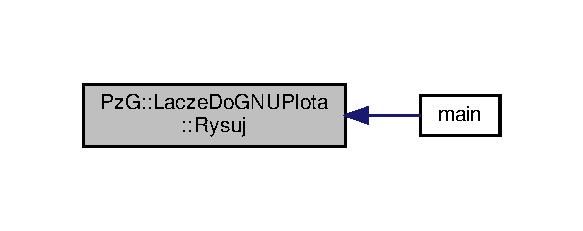
\includegraphics[width=280pt]{class_pz_g_1_1_lacze_do_g_n_u_plota_a065f5b8402737cc62b0ad4f66d028335_icgraph}
\end{center}
\end{figure}
\mbox{\Hypertarget{class_pz_g_1_1_lacze_do_g_n_u_plota_addae9ac156ae2fb227f792faff3aa148}\label{class_pz_g_1_1_lacze_do_g_n_u_plota_addae9ac156ae2fb227f792faff3aa148}} 
\index{Pz\+G\+::\+Lacze\+Do\+G\+N\+U\+Plota@{Pz\+G\+::\+Lacze\+Do\+G\+N\+U\+Plota}!Rysuj\+Do\+Pliku@{Rysuj\+Do\+Pliku}}
\index{Rysuj\+Do\+Pliku@{Rysuj\+Do\+Pliku}!Pz\+G\+::\+Lacze\+Do\+G\+N\+U\+Plota@{Pz\+G\+::\+Lacze\+Do\+G\+N\+U\+Plota}}
\subsubsection{\texorpdfstring{Rysuj\+Do\+Pliku()}{RysujDoPliku()}}
{\footnotesize\ttfamily bool Pz\+G\+::\+Lacze\+Do\+G\+N\+U\+Plota\+::\+Rysuj\+Do\+Pliku (\begin{DoxyParamCaption}\item[{const char $\ast$}]{Nazwa\+Pliku }\end{DoxyParamCaption})}

Działa analogicznie jak metoda \hyperlink{class_pz_g_1_1_lacze_do_g_n_u_plota_a065f5b8402737cc62b0ad4f66d028335}{Rysuj}, z tą różnicą, że rysunek robota składowany jest w pliku o nazwie przekazanej przez parametr {\itshape Nazwa\+Pliku}. Rysunek jest zapisywany w formacie {\itshape P\+NG}.

\begin{DoxyPostcond}{Postcondition}
Lista plików nie powinna być pusta ponadto powinno być możliwe otwarcie do zapisu pliku o nazwie przekazanej przez parametr {\itshape Nazwa\+Pliku}, do której dołączane jest rozszerzenie .ps . Metoda nie wymaga wcześniejszego zainicjowania połączenia z programem {\itshape gnuplot}.
\end{DoxyPostcond}

\begin{DoxyRetVals}{Return values}
{\em true} & -\/ gdy zostają poprawnie wysłane polecenia dla {\itshape gnuplota}. Nie oznacza to jednak, że proces rysowania zakończył się pomyślnie. \\
\hline
{\em false} & -\/ gdy połączenie z gnuplotem nie może zostać poprawnie zainicjalizowane lub gdy lista plików jest pusta lub też gdy nie można otworzyć pliku do zapisu. \\
\hline
\end{DoxyRetVals}


Definition at line 244 of file lacze\+\_\+do\+\_\+gnuplota.\+cpp.

\mbox{\Hypertarget{class_pz_g_1_1_lacze_do_g_n_u_plota_a4b1eb252fd785a5aeff938e7b2dce2b1}\label{class_pz_g_1_1_lacze_do_g_n_u_plota_a4b1eb252fd785a5aeff938e7b2dce2b1}} 
\index{Pz\+G\+::\+Lacze\+Do\+G\+N\+U\+Plota@{Pz\+G\+::\+Lacze\+Do\+G\+N\+U\+Plota}!SkalaX@{SkalaX}}
\index{SkalaX@{SkalaX}!Pz\+G\+::\+Lacze\+Do\+G\+N\+U\+Plota@{Pz\+G\+::\+Lacze\+Do\+G\+N\+U\+Plota}}
\subsubsection{\texorpdfstring{Skala\+X()}{SkalaX()}}
{\footnotesize\ttfamily float Pz\+G\+::\+Lacze\+Do\+G\+N\+U\+Plota\+::\+SkalaX (\begin{DoxyParamCaption}{ }\end{DoxyParamCaption}) const\hspace{0.3cm}{\ttfamily [inline]}}



Udostępnia skalę dla osi {\itshape OX}. 

Udostępnia skalę dla osi {\itshape OX} dla tworzonego rysunku. 

Definition at line 488 of file lacze\+\_\+do\+\_\+gnuplota.\+hh.

\mbox{\Hypertarget{class_pz_g_1_1_lacze_do_g_n_u_plota_a44f922ccbc508d6cd7809c669238dae3}\label{class_pz_g_1_1_lacze_do_g_n_u_plota_a44f922ccbc508d6cd7809c669238dae3}} 
\index{Pz\+G\+::\+Lacze\+Do\+G\+N\+U\+Plota@{Pz\+G\+::\+Lacze\+Do\+G\+N\+U\+Plota}!SkalaZ@{SkalaZ}}
\index{SkalaZ@{SkalaZ}!Pz\+G\+::\+Lacze\+Do\+G\+N\+U\+Plota@{Pz\+G\+::\+Lacze\+Do\+G\+N\+U\+Plota}}
\subsubsection{\texorpdfstring{Skala\+Z()}{SkalaZ()}}
{\footnotesize\ttfamily float Pz\+G\+::\+Lacze\+Do\+G\+N\+U\+Plota\+::\+SkalaZ (\begin{DoxyParamCaption}{ }\end{DoxyParamCaption}) const\hspace{0.3cm}{\ttfamily [inline]}}



Udostępnia skalę dla osi {\itshape OZ}. 

Udostępnia skalę dla osi {\itshape OZ} dla tworzonego rysunku. 

Definition at line 494 of file lacze\+\_\+do\+\_\+gnuplota.\+hh.

\mbox{\Hypertarget{class_pz_g_1_1_lacze_do_g_n_u_plota_a88324c53a70846fb6bc9d918ce21fd56}\label{class_pz_g_1_1_lacze_do_g_n_u_plota_a88324c53a70846fb6bc9d918ce21fd56}} 
\index{Pz\+G\+::\+Lacze\+Do\+G\+N\+U\+Plota@{Pz\+G\+::\+Lacze\+Do\+G\+N\+U\+Plota}!Ustaw\+RotacjeX@{Ustaw\+RotacjeX}}
\index{Ustaw\+RotacjeX@{Ustaw\+RotacjeX}!Pz\+G\+::\+Lacze\+Do\+G\+N\+U\+Plota@{Pz\+G\+::\+Lacze\+Do\+G\+N\+U\+Plota}}
\subsubsection{\texorpdfstring{Ustaw\+Rotacje\+X()}{UstawRotacjeX()}}
{\footnotesize\ttfamily void Pz\+G\+::\+Lacze\+Do\+G\+N\+U\+Plota\+::\+Ustaw\+RotacjeX (\begin{DoxyParamCaption}\item[{float}]{kat\+\_\+x }\end{DoxyParamCaption})\hspace{0.3cm}{\ttfamily [inline]}}



Ustawia rotację wokół osi {\itshape OX}. 

Zadaje kąt rotacji wokół osi {\itshape OX}. Umożliwia to zmianę punktu obserwacji renderowanego rysunku. 
\begin{DoxyParams}{Parameters}
{\em kat\+\_\+x} & -\/ wartość kąta rotacji. Jego wartość podawana jest w stopniach. \\
\hline
\end{DoxyParams}


Definition at line 537 of file lacze\+\_\+do\+\_\+gnuplota.\+hh.

\mbox{\Hypertarget{class_pz_g_1_1_lacze_do_g_n_u_plota_a94d8527fd78048ed6cb32ffb29e5f903}\label{class_pz_g_1_1_lacze_do_g_n_u_plota_a94d8527fd78048ed6cb32ffb29e5f903}} 
\index{Pz\+G\+::\+Lacze\+Do\+G\+N\+U\+Plota@{Pz\+G\+::\+Lacze\+Do\+G\+N\+U\+Plota}!Ustaw\+Rotacje\+XZ@{Ustaw\+Rotacje\+XZ}}
\index{Ustaw\+Rotacje\+XZ@{Ustaw\+Rotacje\+XZ}!Pz\+G\+::\+Lacze\+Do\+G\+N\+U\+Plota@{Pz\+G\+::\+Lacze\+Do\+G\+N\+U\+Plota}}
\subsubsection{\texorpdfstring{Ustaw\+Rotacje\+X\+Z()}{UstawRotacjeXZ()}}
{\footnotesize\ttfamily void Pz\+G\+::\+Lacze\+Do\+G\+N\+U\+Plota\+::\+Ustaw\+Rotacje\+XZ (\begin{DoxyParamCaption}\item[{float}]{kat\+\_\+x,  }\item[{float}]{kat\+\_\+z }\end{DoxyParamCaption})\hspace{0.3cm}{\ttfamily [inline]}}



Ustawia rotację wokół osi {\itshape OX} i {\itshape OZ}. 

Zadaje jednocześnie kąt rotacji wokół osi {\itshape OX} i {\itshape OZ}. Umożliwia to zmianę punktu obserwacji renderowanego rysunku. 
\begin{DoxyParams}{Parameters}
{\em kat\+\_\+x} & -\/ wartość kąta rotacji względem osi {\itshape OX}. Jego wartość podawana jest w stopniach. \\
\hline
{\em kat\+\_\+z} & -\/ wartość kąta rotacji względem osi {\itshape OZ}. Jego wartość podawana jest w stopniach. \\
\hline
\end{DoxyParams}


Definition at line 560 of file lacze\+\_\+do\+\_\+gnuplota.\+hh.

\mbox{\Hypertarget{class_pz_g_1_1_lacze_do_g_n_u_plota_a458399aa2a8f4b3f00ccd5b272857ea1}\label{class_pz_g_1_1_lacze_do_g_n_u_plota_a458399aa2a8f4b3f00ccd5b272857ea1}} 
\index{Pz\+G\+::\+Lacze\+Do\+G\+N\+U\+Plota@{Pz\+G\+::\+Lacze\+Do\+G\+N\+U\+Plota}!Ustaw\+RotacjeZ@{Ustaw\+RotacjeZ}}
\index{Ustaw\+RotacjeZ@{Ustaw\+RotacjeZ}!Pz\+G\+::\+Lacze\+Do\+G\+N\+U\+Plota@{Pz\+G\+::\+Lacze\+Do\+G\+N\+U\+Plota}}
\subsubsection{\texorpdfstring{Ustaw\+Rotacje\+Z()}{UstawRotacjeZ()}}
{\footnotesize\ttfamily void Pz\+G\+::\+Lacze\+Do\+G\+N\+U\+Plota\+::\+Ustaw\+RotacjeZ (\begin{DoxyParamCaption}\item[{float}]{kat\+\_\+z }\end{DoxyParamCaption})\hspace{0.3cm}{\ttfamily [inline]}}



Ustawia rotację wokół osi {\itshape OZ}. 

Zadaje kąt rotacji wokół osi {\itshape OZ}. Umożliwia to zmianę punktu obserwacji renderowanego rysunku. 
\begin{DoxyParams}{Parameters}
{\em kat\+\_\+z} & -\/ wartość kąta rotacji. Jego wartość podawana jest w stopniach. \\
\hline
\end{DoxyParams}


Definition at line 546 of file lacze\+\_\+do\+\_\+gnuplota.\+hh.

\mbox{\Hypertarget{class_pz_g_1_1_lacze_do_g_n_u_plota_a855b8338bfe3e5d294d719f24b11090e}\label{class_pz_g_1_1_lacze_do_g_n_u_plota_a855b8338bfe3e5d294d719f24b11090e}} 
\index{Pz\+G\+::\+Lacze\+Do\+G\+N\+U\+Plota@{Pz\+G\+::\+Lacze\+Do\+G\+N\+U\+Plota}!Ustaw\+SkaleX@{Ustaw\+SkaleX}}
\index{Ustaw\+SkaleX@{Ustaw\+SkaleX}!Pz\+G\+::\+Lacze\+Do\+G\+N\+U\+Plota@{Pz\+G\+::\+Lacze\+Do\+G\+N\+U\+Plota}}
\subsubsection{\texorpdfstring{Ustaw\+Skale\+X()}{UstawSkaleX()}}
{\footnotesize\ttfamily void Pz\+G\+::\+Lacze\+Do\+G\+N\+U\+Plota\+::\+Ustaw\+SkaleX (\begin{DoxyParamCaption}\item[{float}]{skala\+\_\+x }\end{DoxyParamCaption})\hspace{0.3cm}{\ttfamily [inline]}}



Zadaje skalę wzdłuż osi {\itshape OZ}. 

Zadaje skalę wzdłuż osi {\itshape OX} dla tworzonego rysunku. 
\begin{DoxyParams}{Parameters}
{\em skala\+\_\+x} & -\/ skala wzdłuż osi {\itshape OX}. \\
\hline
\end{DoxyParams}


Definition at line 501 of file lacze\+\_\+do\+\_\+gnuplota.\+hh.

\mbox{\Hypertarget{class_pz_g_1_1_lacze_do_g_n_u_plota_a4308151b54e105d302803146a3238699}\label{class_pz_g_1_1_lacze_do_g_n_u_plota_a4308151b54e105d302803146a3238699}} 
\index{Pz\+G\+::\+Lacze\+Do\+G\+N\+U\+Plota@{Pz\+G\+::\+Lacze\+Do\+G\+N\+U\+Plota}!Ustaw\+Skale\+XZ@{Ustaw\+Skale\+XZ}}
\index{Ustaw\+Skale\+XZ@{Ustaw\+Skale\+XZ}!Pz\+G\+::\+Lacze\+Do\+G\+N\+U\+Plota@{Pz\+G\+::\+Lacze\+Do\+G\+N\+U\+Plota}}
\subsubsection{\texorpdfstring{Ustaw\+Skale\+X\+Z()}{UstawSkaleXZ()}}
{\footnotesize\ttfamily void Pz\+G\+::\+Lacze\+Do\+G\+N\+U\+Plota\+::\+Ustaw\+Skale\+XZ (\begin{DoxyParamCaption}\item[{float}]{skala\+\_\+x,  }\item[{float}]{skala\+\_\+z }\end{DoxyParamCaption})\hspace{0.3cm}{\ttfamily [inline]}}



Zadaje skalę wzdłuż osi {\itshape OX} i {\itshape OZ}. 

Zadaje skalę wzdłuż osi {\itshape OX} i {\itshape OZ} dla tworzonego rysunku. 
\begin{DoxyParams}{Parameters}
{\em skala\+\_\+x} & -\/ skala wzdłuż osi {\itshape OX}. \\
\hline
{\em skala\+\_\+z} & -\/ skala wzdłuż osi {\itshape OZ}. \\
\hline
\end{DoxyParams}


Definition at line 516 of file lacze\+\_\+do\+\_\+gnuplota.\+hh.

\mbox{\Hypertarget{class_pz_g_1_1_lacze_do_g_n_u_plota_ab0486db3166d8db6580a221079af241f}\label{class_pz_g_1_1_lacze_do_g_n_u_plota_ab0486db3166d8db6580a221079af241f}} 
\index{Pz\+G\+::\+Lacze\+Do\+G\+N\+U\+Plota@{Pz\+G\+::\+Lacze\+Do\+G\+N\+U\+Plota}!Ustaw\+SkaleZ@{Ustaw\+SkaleZ}}
\index{Ustaw\+SkaleZ@{Ustaw\+SkaleZ}!Pz\+G\+::\+Lacze\+Do\+G\+N\+U\+Plota@{Pz\+G\+::\+Lacze\+Do\+G\+N\+U\+Plota}}
\subsubsection{\texorpdfstring{Ustaw\+Skale\+Z()}{UstawSkaleZ()}}
{\footnotesize\ttfamily void Pz\+G\+::\+Lacze\+Do\+G\+N\+U\+Plota\+::\+Ustaw\+SkaleZ (\begin{DoxyParamCaption}\item[{float}]{skala\+\_\+z }\end{DoxyParamCaption})\hspace{0.3cm}{\ttfamily [inline]}}



Zadaje skalę wzdłuż osi {\itshape OZ}. 

Zadaje skalę wzdłuż osi {\itshape OZ} dla tworzonego rysunku. 
\begin{DoxyParams}{Parameters}
{\em skala\+\_\+z} & -\/ skala wzdłuż osi {\itshape OZ}. \\
\hline
\end{DoxyParams}


Definition at line 508 of file lacze\+\_\+do\+\_\+gnuplota.\+hh.

\mbox{\Hypertarget{class_pz_g_1_1_lacze_do_g_n_u_plota_a9c91987dfc869d6fcea96205c581daef}\label{class_pz_g_1_1_lacze_do_g_n_u_plota_a9c91987dfc869d6fcea96205c581daef}} 
\index{Pz\+G\+::\+Lacze\+Do\+G\+N\+U\+Plota@{Pz\+G\+::\+Lacze\+Do\+G\+N\+U\+Plota}!Ustaw\+ZakresX@{Ustaw\+ZakresX}}
\index{Ustaw\+ZakresX@{Ustaw\+ZakresX}!Pz\+G\+::\+Lacze\+Do\+G\+N\+U\+Plota@{Pz\+G\+::\+Lacze\+Do\+G\+N\+U\+Plota}}
\subsubsection{\texorpdfstring{Ustaw\+Zakres\+X()}{UstawZakresX()}}
{\footnotesize\ttfamily void Pz\+G\+::\+Lacze\+Do\+G\+N\+U\+Plota\+::\+Ustaw\+ZakresX (\begin{DoxyParamCaption}\item[{float}]{Xo,  }\item[{float}]{Xn }\end{DoxyParamCaption})\hspace{0.3cm}{\ttfamily [inline]}}



Ustawia zakres osi {\itshape OX}. 

Ustawia zakres osi {\itshape OX}. Ogranicza to obszar, który będzie zwizualizowany przez programa {\itshape gnuplot}. 
\begin{DoxyParams}{Parameters}
{\em Xo} & -\/ dolna granica obszaru rysowania dla osi {\itshape OX}. \\
\hline
{\em Xn} & -\/ górna granica obszaru rysowania dla osi {\itshape OX}. \\
\hline
\end{DoxyParams}


Definition at line 462 of file lacze\+\_\+do\+\_\+gnuplota.\+hh.

Here is the caller graph for this function\+:\nopagebreak
\begin{figure}[H]
\begin{center}
\leavevmode
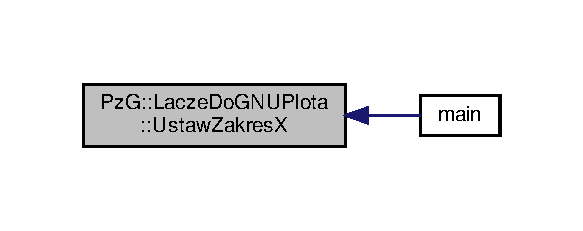
\includegraphics[width=280pt]{class_pz_g_1_1_lacze_do_g_n_u_plota_a9c91987dfc869d6fcea96205c581daef_icgraph}
\end{center}
\end{figure}
\mbox{\Hypertarget{class_pz_g_1_1_lacze_do_g_n_u_plota_a54c6e9cf9ab2eae479451fd953c2717c}\label{class_pz_g_1_1_lacze_do_g_n_u_plota_a54c6e9cf9ab2eae479451fd953c2717c}} 
\index{Pz\+G\+::\+Lacze\+Do\+G\+N\+U\+Plota@{Pz\+G\+::\+Lacze\+Do\+G\+N\+U\+Plota}!Ustaw\+ZakresY@{Ustaw\+ZakresY}}
\index{Ustaw\+ZakresY@{Ustaw\+ZakresY}!Pz\+G\+::\+Lacze\+Do\+G\+N\+U\+Plota@{Pz\+G\+::\+Lacze\+Do\+G\+N\+U\+Plota}}
\subsubsection{\texorpdfstring{Ustaw\+Zakres\+Y()}{UstawZakresY()}}
{\footnotesize\ttfamily void Pz\+G\+::\+Lacze\+Do\+G\+N\+U\+Plota\+::\+Ustaw\+ZakresY (\begin{DoxyParamCaption}\item[{float}]{Yo,  }\item[{float}]{Yn }\end{DoxyParamCaption})\hspace{0.3cm}{\ttfamily [inline]}}



Ustawia zakres osi {\itshape OY}. 

Ustawia zakres osi {\itshape OY}. Ogranicza to obszar, który będzie zwizualizowany przez programa {\itshape gnuplot}. 
\begin{DoxyParams}{Parameters}
{\em Yo} & -\/ dolna granica obszaru rysowania dla osi {\itshape OY}. \\
\hline
{\em Yn} & -\/ górna granica obszaru rysowania dla osi {\itshape OY}. \\
\hline
\end{DoxyParams}


Definition at line 471 of file lacze\+\_\+do\+\_\+gnuplota.\+hh.

Here is the caller graph for this function\+:\nopagebreak
\begin{figure}[H]
\begin{center}
\leavevmode
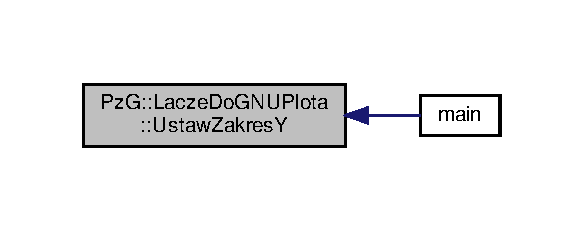
\includegraphics[width=280pt]{class_pz_g_1_1_lacze_do_g_n_u_plota_a54c6e9cf9ab2eae479451fd953c2717c_icgraph}
\end{center}
\end{figure}
\mbox{\Hypertarget{class_pz_g_1_1_lacze_do_g_n_u_plota_a1dbbb2b86fb13b8632e6bad9df2a82e3}\label{class_pz_g_1_1_lacze_do_g_n_u_plota_a1dbbb2b86fb13b8632e6bad9df2a82e3}} 
\index{Pz\+G\+::\+Lacze\+Do\+G\+N\+U\+Plota@{Pz\+G\+::\+Lacze\+Do\+G\+N\+U\+Plota}!Ustaw\+ZakresZ@{Ustaw\+ZakresZ}}
\index{Ustaw\+ZakresZ@{Ustaw\+ZakresZ}!Pz\+G\+::\+Lacze\+Do\+G\+N\+U\+Plota@{Pz\+G\+::\+Lacze\+Do\+G\+N\+U\+Plota}}
\subsubsection{\texorpdfstring{Ustaw\+Zakres\+Z()}{UstawZakresZ()}}
{\footnotesize\ttfamily void Pz\+G\+::\+Lacze\+Do\+G\+N\+U\+Plota\+::\+Ustaw\+ZakresZ (\begin{DoxyParamCaption}\item[{float}]{Zo,  }\item[{float}]{Zn }\end{DoxyParamCaption})\hspace{0.3cm}{\ttfamily [inline]}}



Ustawia zakres osi {\itshape OZ}. 

Ustawia zakres osi {\itshape OZ}. Ogranicza to obszar, który będzie zwizualizowany przez programa {\itshape gnuplot}. 
\begin{DoxyParams}{Parameters}
{\em Zo} & -\/ dolna granica obszaru rysowania dla osi {\itshape OZ}. \\
\hline
{\em Zn} & -\/ górna granica obszaru rysowania dla osi {\itshape OZ}. \\
\hline
\end{DoxyParams}


Definition at line 480 of file lacze\+\_\+do\+\_\+gnuplota.\+hh.

Here is the caller graph for this function\+:\nopagebreak
\begin{figure}[H]
\begin{center}
\leavevmode
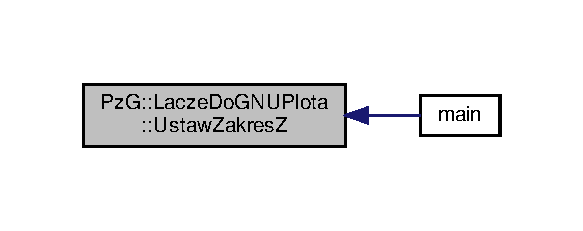
\includegraphics[width=280pt]{class_pz_g_1_1_lacze_do_g_n_u_plota_a1dbbb2b86fb13b8632e6bad9df2a82e3_icgraph}
\end{center}
\end{figure}
\mbox{\Hypertarget{class_pz_g_1_1_lacze_do_g_n_u_plota_a75f599f17413ea8602c6dbba09f36407}\label{class_pz_g_1_1_lacze_do_g_n_u_plota_a75f599f17413ea8602c6dbba09f36407}} 
\index{Pz\+G\+::\+Lacze\+Do\+G\+N\+U\+Plota@{Pz\+G\+::\+Lacze\+Do\+G\+N\+U\+Plota}!Usun\+Ostatnia\+Nazwe@{Usun\+Ostatnia\+Nazwe}}
\index{Usun\+Ostatnia\+Nazwe@{Usun\+Ostatnia\+Nazwe}!Pz\+G\+::\+Lacze\+Do\+G\+N\+U\+Plota@{Pz\+G\+::\+Lacze\+Do\+G\+N\+U\+Plota}}
\subsubsection{\texorpdfstring{Usun\+Ostatnia\+Nazwe()}{UsunOstatniaNazwe()}}
{\footnotesize\ttfamily void Pz\+G\+::\+Lacze\+Do\+G\+N\+U\+Plota\+::\+Usun\+Ostatnia\+Nazwe (\begin{DoxyParamCaption}{ }\end{DoxyParamCaption})}



Usuwa ostatnią nazwę pliku. 

Usuwa ostatnią nazwę z listy nazw plików. 

Definition at line 440 of file lacze\+\_\+do\+\_\+gnuplota.\+cpp.

\mbox{\Hypertarget{class_pz_g_1_1_lacze_do_g_n_u_plota_a89a1d90d017d264cd26398464d074073}\label{class_pz_g_1_1_lacze_do_g_n_u_plota_a89a1d90d017d264cd26398464d074073}} 
\index{Pz\+G\+::\+Lacze\+Do\+G\+N\+U\+Plota@{Pz\+G\+::\+Lacze\+Do\+G\+N\+U\+Plota}!Usun\+Wszystkie\+Nazwy\+Plikow@{Usun\+Wszystkie\+Nazwy\+Plikow}}
\index{Usun\+Wszystkie\+Nazwy\+Plikow@{Usun\+Wszystkie\+Nazwy\+Plikow}!Pz\+G\+::\+Lacze\+Do\+G\+N\+U\+Plota@{Pz\+G\+::\+Lacze\+Do\+G\+N\+U\+Plota}}
\subsubsection{\texorpdfstring{Usun\+Wszystkie\+Nazwy\+Plikow()}{UsunWszystkieNazwyPlikow()}}
{\footnotesize\ttfamily void Pz\+G\+::\+Lacze\+Do\+G\+N\+U\+Plota\+::\+Usun\+Wszystkie\+Nazwy\+Plikow (\begin{DoxyParamCaption}{ }\end{DoxyParamCaption})}



Kasuje zawartość listy nazw plików. 

Calkowicie kasuje zawartość listy nazw plików. 

Definition at line 451 of file lacze\+\_\+do\+\_\+gnuplota.\+cpp.

\mbox{\Hypertarget{class_pz_g_1_1_lacze_do_g_n_u_plota_a1c7b9acc40de8d8bbb40fb0722512933}\label{class_pz_g_1_1_lacze_do_g_n_u_plota_a1c7b9acc40de8d8bbb40fb0722512933}} 
\index{Pz\+G\+::\+Lacze\+Do\+G\+N\+U\+Plota@{Pz\+G\+::\+Lacze\+Do\+G\+N\+U\+Plota}!Utworz\+Proces\+Potomny@{Utworz\+Proces\+Potomny}}
\index{Utworz\+Proces\+Potomny@{Utworz\+Proces\+Potomny}!Pz\+G\+::\+Lacze\+Do\+G\+N\+U\+Plota@{Pz\+G\+::\+Lacze\+Do\+G\+N\+U\+Plota}}
\subsubsection{\texorpdfstring{Utworz\+Proces\+Potomny()}{UtworzProcesPotomny()}}
{\footnotesize\ttfamily bool Pz\+G\+::\+Lacze\+Do\+G\+N\+U\+Plota\+::\+Utworz\+Proces\+Potomny (\begin{DoxyParamCaption}{ }\end{DoxyParamCaption})\hspace{0.3cm}{\ttfamily [protected]}}



Uruchamia program {\itshape gnuplot} jako proces potomny. 

Inicjalizuje połączenie z programem {\itshape gnuplot}. Realizowane jest to poprzez rozwidlenie procesu i uruchomienie jako procesu potomnego programu {\itshape gnuplot}. Komunikacja z programem {\itshape gnuplot} realizowana jest poprzez przejęcie jego wejścia i wyjścia standardowego.


\begin{DoxyRetVals}{Return values}
{\em true} & -\/ gdy połączenie z programem {\itshape gnuplot} zostało poprawnie zainicjalizowane lub gdy już wcześniej było zainicjalizowane. \\
\hline
{\em false} & -\/ gdy proces inicjalizacji połączenia zakończył się niepowodzeniem. \\
\hline
\end{DoxyRetVals}


Definition at line 162 of file lacze\+\_\+do\+\_\+gnuplota.\+cpp.

\mbox{\Hypertarget{class_pz_g_1_1_lacze_do_g_n_u_plota_a7c417f27b4b112f58a5be3ce6ea8d1fe}\label{class_pz_g_1_1_lacze_do_g_n_u_plota_a7c417f27b4b112f58a5be3ce6ea8d1fe}} 
\index{Pz\+G\+::\+Lacze\+Do\+G\+N\+U\+Plota@{Pz\+G\+::\+Lacze\+Do\+G\+N\+U\+Plota}!Wez\+Tryb\+Rys@{Wez\+Tryb\+Rys}}
\index{Wez\+Tryb\+Rys@{Wez\+Tryb\+Rys}!Pz\+G\+::\+Lacze\+Do\+G\+N\+U\+Plota@{Pz\+G\+::\+Lacze\+Do\+G\+N\+U\+Plota}}
\subsubsection{\texorpdfstring{Wez\+Tryb\+Rys()}{WezTrybRys()}}
{\footnotesize\ttfamily \hyperlink{namespace_pz_g_aeedae1ef10c66d720f9e89de408ca4ca}{Tryb\+Rysowania} Pz\+G\+::\+Lacze\+Do\+G\+N\+U\+Plota\+::\+Wez\+Tryb\+Rys (\begin{DoxyParamCaption}{ }\end{DoxyParamCaption}) const\hspace{0.3cm}{\ttfamily [inline]}}



Udostępnia aktualny tryb rysowania. 

Udostępnia informację o aktualnym trybie rysowania. 

Definition at line 452 of file lacze\+\_\+do\+\_\+gnuplota.\+hh.

\mbox{\Hypertarget{class_pz_g_1_1_lacze_do_g_n_u_plota_a4531e6d166faf2e2c8bb4a54a9c9e1f8}\label{class_pz_g_1_1_lacze_do_g_n_u_plota_a4531e6d166faf2e2c8bb4a54a9c9e1f8}} 
\index{Pz\+G\+::\+Lacze\+Do\+G\+N\+U\+Plota@{Pz\+G\+::\+Lacze\+Do\+G\+N\+U\+Plota}!Wyswietlaj\+Komunikaty\+Bledow@{Wyswietlaj\+Komunikaty\+Bledow}}
\index{Wyswietlaj\+Komunikaty\+Bledow@{Wyswietlaj\+Komunikaty\+Bledow}!Pz\+G\+::\+Lacze\+Do\+G\+N\+U\+Plota@{Pz\+G\+::\+Lacze\+Do\+G\+N\+U\+Plota}}
\subsubsection{\texorpdfstring{Wyswietlaj\+Komunikaty\+Bledow()}{WyswietlajKomunikatyBledow()}}
{\footnotesize\ttfamily void Pz\+G\+::\+Lacze\+Do\+G\+N\+U\+Plota\+::\+Wyswietlaj\+Komunikaty\+Bledow (\begin{DoxyParamCaption}\item[{bool}]{Tryb = {\ttfamily true} }\end{DoxyParamCaption})}



Zezwala lub zabrania wyświetlania komunikatów. 

Metoda pozwala, albo też zabrania wyświetlania komunikatów o blędach. Jeżeli jakaś z operacji nie powiedzie się, to jako wynik zwracana jest wartość {\ttfamily false}. Oprócz tego metody takie moga wyświetlać komunikaty, które kierowane są na wyjście \char`\"{}standard error\char`\"{} Domyślnie przymuje się, że programista nie chce dodatkwego wyświetlania komunikatów. 

Definition at line 29 of file lacze\+\_\+do\+\_\+gnuplota.\+cpp.

\mbox{\Hypertarget{class_pz_g_1_1_lacze_do_g_n_u_plota_a8e23479629af3df3d352b7839ae396b8}\label{class_pz_g_1_1_lacze_do_g_n_u_plota_a8e23479629af3df3d352b7839ae396b8}} 
\index{Pz\+G\+::\+Lacze\+Do\+G\+N\+U\+Plota@{Pz\+G\+::\+Lacze\+Do\+G\+N\+U\+Plota}!Xmax@{Xmax}}
\index{Xmax@{Xmax}!Pz\+G\+::\+Lacze\+Do\+G\+N\+U\+Plota@{Pz\+G\+::\+Lacze\+Do\+G\+N\+U\+Plota}}
\subsubsection{\texorpdfstring{Xmax()}{Xmax()}}
{\footnotesize\ttfamily float Pz\+G\+::\+Lacze\+Do\+G\+N\+U\+Plota\+::\+Xmax (\begin{DoxyParamCaption}{ }\end{DoxyParamCaption}) const\hspace{0.3cm}{\ttfamily [inline]}}

Udostępnia górną wartość zakresu skali wzdłuż osi {\itshape OX}. 

Definition at line 420 of file lacze\+\_\+do\+\_\+gnuplota.\+hh.

\mbox{\Hypertarget{class_pz_g_1_1_lacze_do_g_n_u_plota_a66836c9749bf179420e4ca3e9447efd7}\label{class_pz_g_1_1_lacze_do_g_n_u_plota_a66836c9749bf179420e4ca3e9447efd7}} 
\index{Pz\+G\+::\+Lacze\+Do\+G\+N\+U\+Plota@{Pz\+G\+::\+Lacze\+Do\+G\+N\+U\+Plota}!Xmin@{Xmin}}
\index{Xmin@{Xmin}!Pz\+G\+::\+Lacze\+Do\+G\+N\+U\+Plota@{Pz\+G\+::\+Lacze\+Do\+G\+N\+U\+Plota}}
\subsubsection{\texorpdfstring{Xmin()}{Xmin()}}
{\footnotesize\ttfamily float Pz\+G\+::\+Lacze\+Do\+G\+N\+U\+Plota\+::\+Xmin (\begin{DoxyParamCaption}{ }\end{DoxyParamCaption}) const\hspace{0.3cm}{\ttfamily [inline]}}

Udostępnia dolną wartość zakresu skali wzdłuż osi {\itshape OX}. 

Definition at line 416 of file lacze\+\_\+do\+\_\+gnuplota.\+hh.

\mbox{\Hypertarget{class_pz_g_1_1_lacze_do_g_n_u_plota_ac54e4e7448ce3bd324efdc94a999f535}\label{class_pz_g_1_1_lacze_do_g_n_u_plota_ac54e4e7448ce3bd324efdc94a999f535}} 
\index{Pz\+G\+::\+Lacze\+Do\+G\+N\+U\+Plota@{Pz\+G\+::\+Lacze\+Do\+G\+N\+U\+Plota}!Ymax@{Ymax}}
\index{Ymax@{Ymax}!Pz\+G\+::\+Lacze\+Do\+G\+N\+U\+Plota@{Pz\+G\+::\+Lacze\+Do\+G\+N\+U\+Plota}}
\subsubsection{\texorpdfstring{Ymax()}{Ymax()}}
{\footnotesize\ttfamily float Pz\+G\+::\+Lacze\+Do\+G\+N\+U\+Plota\+::\+Ymax (\begin{DoxyParamCaption}{ }\end{DoxyParamCaption}) const\hspace{0.3cm}{\ttfamily [inline]}}

Udostępnia górną wartość zakresu skali wzdłuż osi {\itshape OY}. 

Definition at line 428 of file lacze\+\_\+do\+\_\+gnuplota.\+hh.

\mbox{\Hypertarget{class_pz_g_1_1_lacze_do_g_n_u_plota_a9352c0382bfaeaaba9f65399a7383164}\label{class_pz_g_1_1_lacze_do_g_n_u_plota_a9352c0382bfaeaaba9f65399a7383164}} 
\index{Pz\+G\+::\+Lacze\+Do\+G\+N\+U\+Plota@{Pz\+G\+::\+Lacze\+Do\+G\+N\+U\+Plota}!Ymin@{Ymin}}
\index{Ymin@{Ymin}!Pz\+G\+::\+Lacze\+Do\+G\+N\+U\+Plota@{Pz\+G\+::\+Lacze\+Do\+G\+N\+U\+Plota}}
\subsubsection{\texorpdfstring{Ymin()}{Ymin()}}
{\footnotesize\ttfamily float Pz\+G\+::\+Lacze\+Do\+G\+N\+U\+Plota\+::\+Ymin (\begin{DoxyParamCaption}{ }\end{DoxyParamCaption}) const\hspace{0.3cm}{\ttfamily [inline]}}

Udostępnia dolną wartość zakresu skali wzdłuż osi {\itshape OY}. 

Definition at line 424 of file lacze\+\_\+do\+\_\+gnuplota.\+hh.

\mbox{\Hypertarget{class_pz_g_1_1_lacze_do_g_n_u_plota_aa92b463e8cbae31b50dd797a4183bce8}\label{class_pz_g_1_1_lacze_do_g_n_u_plota_aa92b463e8cbae31b50dd797a4183bce8}} 
\index{Pz\+G\+::\+Lacze\+Do\+G\+N\+U\+Plota@{Pz\+G\+::\+Lacze\+Do\+G\+N\+U\+Plota}!Zapisz\+Ustawienie\+Rotacji\+I\+Skali@{Zapisz\+Ustawienie\+Rotacji\+I\+Skali}}
\index{Zapisz\+Ustawienie\+Rotacji\+I\+Skali@{Zapisz\+Ustawienie\+Rotacji\+I\+Skali}!Pz\+G\+::\+Lacze\+Do\+G\+N\+U\+Plota@{Pz\+G\+::\+Lacze\+Do\+G\+N\+U\+Plota}}
\subsubsection{\texorpdfstring{Zapisz\+Ustawienie\+Rotacji\+I\+Skali()}{ZapiszUstawienieRotacjiISkali()}}
{\footnotesize\ttfamily std\+::string Pz\+G\+::\+Lacze\+Do\+G\+N\+U\+Plota\+::\+Zapisz\+Ustawienie\+Rotacji\+I\+Skali (\begin{DoxyParamCaption}{ }\end{DoxyParamCaption}) const\hspace{0.3cm}{\ttfamily [protected]}}



Tworzy polecenie ustawiające punkt obserwacji. 

Tworzy polecenie dla programu {\itshape gnuplot} ustawiajające punkt obserwacji poprzez zadanie rotacji i skali dla poszczególnych osi. 

Definition at line 423 of file lacze\+\_\+do\+\_\+gnuplota.\+cpp.

\mbox{\Hypertarget{class_pz_g_1_1_lacze_do_g_n_u_plota_a4579aecf7b4777fdde0cae4e98c275c2}\label{class_pz_g_1_1_lacze_do_g_n_u_plota_a4579aecf7b4777fdde0cae4e98c275c2}} 
\index{Pz\+G\+::\+Lacze\+Do\+G\+N\+U\+Plota@{Pz\+G\+::\+Lacze\+Do\+G\+N\+U\+Plota}!Zapisz\+Ustawienie\+Zakresu@{Zapisz\+Ustawienie\+Zakresu}}
\index{Zapisz\+Ustawienie\+Zakresu@{Zapisz\+Ustawienie\+Zakresu}!Pz\+G\+::\+Lacze\+Do\+G\+N\+U\+Plota@{Pz\+G\+::\+Lacze\+Do\+G\+N\+U\+Plota}}
\subsubsection{\texorpdfstring{Zapisz\+Ustawienie\+Zakresu()}{ZapiszUstawienieZakresu()}}
{\footnotesize\ttfamily std\+::string Pz\+G\+::\+Lacze\+Do\+G\+N\+U\+Plota\+::\+Zapisz\+Ustawienie\+Zakresu (\begin{DoxyParamCaption}\item[{char}]{Os }\end{DoxyParamCaption}) const\hspace{0.3cm}{\ttfamily [protected]}}



Tworzy polecenie ustawiające zakres dla danej współrzędnej. 

Tworzy polecenie dla programu {\itshape gnuplot} ustawiające zakres współrzędnych wybranej współrzędnej {\itshape x}, {\itshape y} lub {\itshape z}, dla której ma być tworzony dany rysunek. 
\begin{DoxyParams}{Parameters}
{\em Os} & -\/ zawiera znak określający współrzędną, dla której ma zostać wygenerowane polecenie ustawienia zakresu. \\
\hline
\end{DoxyParams}
\begin{DoxyReturn}{Returns}
łańcuch znaków polecenia ustawiającego żądany zakres dla wybranej współrzędnej. 
\end{DoxyReturn}


Definition at line 404 of file lacze\+\_\+do\+\_\+gnuplota.\+cpp.

\mbox{\Hypertarget{class_pz_g_1_1_lacze_do_g_n_u_plota_a20a5d03e1fc19c682032bffc54340f12}\label{class_pz_g_1_1_lacze_do_g_n_u_plota_a20a5d03e1fc19c682032bffc54340f12}} 
\index{Pz\+G\+::\+Lacze\+Do\+G\+N\+U\+Plota@{Pz\+G\+::\+Lacze\+Do\+G\+N\+U\+Plota}!Zmax@{Zmax}}
\index{Zmax@{Zmax}!Pz\+G\+::\+Lacze\+Do\+G\+N\+U\+Plota@{Pz\+G\+::\+Lacze\+Do\+G\+N\+U\+Plota}}
\subsubsection{\texorpdfstring{Zmax()}{Zmax()}}
{\footnotesize\ttfamily float Pz\+G\+::\+Lacze\+Do\+G\+N\+U\+Plota\+::\+Zmax (\begin{DoxyParamCaption}{ }\end{DoxyParamCaption}) const\hspace{0.3cm}{\ttfamily [inline]}}

Udostępnia górną wartość zakresu skali wzdłuż osi {\itshape OZ}. 

Definition at line 436 of file lacze\+\_\+do\+\_\+gnuplota.\+hh.

\mbox{\Hypertarget{class_pz_g_1_1_lacze_do_g_n_u_plota_a10950349b348fd3a3d4143e95337527c}\label{class_pz_g_1_1_lacze_do_g_n_u_plota_a10950349b348fd3a3d4143e95337527c}} 
\index{Pz\+G\+::\+Lacze\+Do\+G\+N\+U\+Plota@{Pz\+G\+::\+Lacze\+Do\+G\+N\+U\+Plota}!Zmien\+Tryb\+Rys@{Zmien\+Tryb\+Rys}}
\index{Zmien\+Tryb\+Rys@{Zmien\+Tryb\+Rys}!Pz\+G\+::\+Lacze\+Do\+G\+N\+U\+Plota@{Pz\+G\+::\+Lacze\+Do\+G\+N\+U\+Plota}}
\subsubsection{\texorpdfstring{Zmien\+Tryb\+Rys()}{ZmienTrybRys()}}
{\footnotesize\ttfamily void Pz\+G\+::\+Lacze\+Do\+G\+N\+U\+Plota\+::\+Zmien\+Tryb\+Rys (\begin{DoxyParamCaption}\item[{\hyperlink{namespace_pz_g_aeedae1ef10c66d720f9e89de408ca4ca}{Tryb\+Rysowania}}]{Tryb }\end{DoxyParamCaption})\hspace{0.3cm}{\ttfamily [inline]}}



Zmienia tryb rysowania. 

Zmienia tryb rysowania jaki zostanie wymuszony na programie {\ttfamily gnuplot}. 
\begin{DoxyParams}{Parameters}
{\em Tryb} & -\/ wartość parametru określa nowy tryb rysowania. \\
\hline
\end{DoxyParams}


Definition at line 445 of file lacze\+\_\+do\+\_\+gnuplota.\+hh.

Here is the caller graph for this function\+:\nopagebreak
\begin{figure}[H]
\begin{center}
\leavevmode
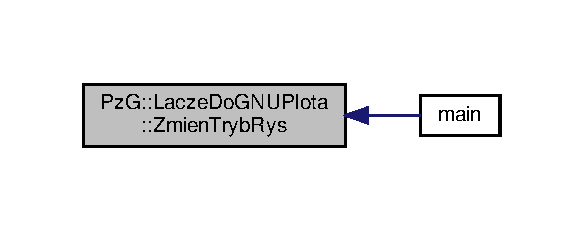
\includegraphics[width=280pt]{class_pz_g_1_1_lacze_do_g_n_u_plota_a10950349b348fd3a3d4143e95337527c_icgraph}
\end{center}
\end{figure}
\mbox{\Hypertarget{class_pz_g_1_1_lacze_do_g_n_u_plota_a9068bd9a9873ba9c6d70016f1ae7cd7f}\label{class_pz_g_1_1_lacze_do_g_n_u_plota_a9068bd9a9873ba9c6d70016f1ae7cd7f}} 
\index{Pz\+G\+::\+Lacze\+Do\+G\+N\+U\+Plota@{Pz\+G\+::\+Lacze\+Do\+G\+N\+U\+Plota}!Zmin@{Zmin}}
\index{Zmin@{Zmin}!Pz\+G\+::\+Lacze\+Do\+G\+N\+U\+Plota@{Pz\+G\+::\+Lacze\+Do\+G\+N\+U\+Plota}}
\subsubsection{\texorpdfstring{Zmin()}{Zmin()}}
{\footnotesize\ttfamily float Pz\+G\+::\+Lacze\+Do\+G\+N\+U\+Plota\+::\+Zmin (\begin{DoxyParamCaption}{ }\end{DoxyParamCaption}) const\hspace{0.3cm}{\ttfamily [inline]}}

Udostępnia dolną wartość zakresu skali wzdłuż osi {\itshape OZ}. 

Definition at line 432 of file lacze\+\_\+do\+\_\+gnuplota.\+hh.



\subsection{Member Data Documentation}
\mbox{\Hypertarget{class_pz_g_1_1_lacze_do_g_n_u_plota_a1916c5a6fecfb3554e9d5204b2f2086c}\label{class_pz_g_1_1_lacze_do_g_n_u_plota_a1916c5a6fecfb3554e9d5204b2f2086c}} 
\index{Pz\+G\+::\+Lacze\+Do\+G\+N\+U\+Plota@{Pz\+G\+::\+Lacze\+Do\+G\+N\+U\+Plota}!\+\_\+\+Info\+Plikow@{\+\_\+\+Info\+Plikow}}
\index{\+\_\+\+Info\+Plikow@{\+\_\+\+Info\+Plikow}!Pz\+G\+::\+Lacze\+Do\+G\+N\+U\+Plota@{Pz\+G\+::\+Lacze\+Do\+G\+N\+U\+Plota}}
\subsubsection{\texorpdfstring{\+\_\+\+Info\+Plikow}{\_InfoPlikow}}
{\footnotesize\ttfamily std\+::list$<$ \hyperlink{class_pz_g_1_1_info_pliku_do_rysowania}{Info\+Pliku\+Do\+Rysowania} $>$ Pz\+G\+::\+Lacze\+Do\+G\+N\+U\+Plota\+::\+\_\+\+Info\+Plikow\hspace{0.3cm}{\ttfamily [static]}, {\ttfamily [protected]}}



Lista nazw plików z danymi dla {\itshape gnuplota}. 

Pole jest zarządcą listy nazw plików, z których są wczytywane dane dotyczące rysowania obrysu brył przez program {\itshape gnuplot}. Operacja ta wykonywana jest po wywołaniu polecenia. \hyperlink{class_pz_g_1_1_lacze_do_g_n_u_plota_a065f5b8402737cc62b0ad4f66d028335}{Rysuj}. 

Definition at line 136 of file lacze\+\_\+do\+\_\+gnuplota.\+hh.

\mbox{\Hypertarget{class_pz_g_1_1_lacze_do_g_n_u_plota_a833aa8994b9913786f920ec8c259731f}\label{class_pz_g_1_1_lacze_do_g_n_u_plota_a833aa8994b9913786f920ec8c259731f}} 
\index{Pz\+G\+::\+Lacze\+Do\+G\+N\+U\+Plota@{Pz\+G\+::\+Lacze\+Do\+G\+N\+U\+Plota}!\+\_\+\+Pokaz\+Os\+\_\+\+OX@{\+\_\+\+Pokaz\+Os\+\_\+\+OX}}
\index{\+\_\+\+Pokaz\+Os\+\_\+\+OX@{\+\_\+\+Pokaz\+Os\+\_\+\+OX}!Pz\+G\+::\+Lacze\+Do\+G\+N\+U\+Plota@{Pz\+G\+::\+Lacze\+Do\+G\+N\+U\+Plota}}
\subsubsection{\texorpdfstring{\+\_\+\+Pokaz\+Os\+\_\+\+OX}{\_PokazOs\_OX}}
{\footnotesize\ttfamily bool Pz\+G\+::\+Lacze\+Do\+G\+N\+U\+Plota\+::\+\_\+\+Pokaz\+Os\+\_\+\+OX\hspace{0.3cm}{\ttfamily [protected]}}



Czy oś OX ma być widoczna. 

Przechowuje informację decydującą o tym czy oś OX będzie widoczna na rysunku ({\ttfamily true}), czy też nie ({\ttfamily false}). 

Definition at line 232 of file lacze\+\_\+do\+\_\+gnuplota.\+hh.

\mbox{\Hypertarget{class_pz_g_1_1_lacze_do_g_n_u_plota_ae8d9b4dac5eae6ce86b7043c45b70ed8}\label{class_pz_g_1_1_lacze_do_g_n_u_plota_ae8d9b4dac5eae6ce86b7043c45b70ed8}} 
\index{Pz\+G\+::\+Lacze\+Do\+G\+N\+U\+Plota@{Pz\+G\+::\+Lacze\+Do\+G\+N\+U\+Plota}!\+\_\+\+Pokaz\+Os\+\_\+\+OY@{\+\_\+\+Pokaz\+Os\+\_\+\+OY}}
\index{\+\_\+\+Pokaz\+Os\+\_\+\+OY@{\+\_\+\+Pokaz\+Os\+\_\+\+OY}!Pz\+G\+::\+Lacze\+Do\+G\+N\+U\+Plota@{Pz\+G\+::\+Lacze\+Do\+G\+N\+U\+Plota}}
\subsubsection{\texorpdfstring{\+\_\+\+Pokaz\+Os\+\_\+\+OY}{\_PokazOs\_OY}}
{\footnotesize\ttfamily bool Pz\+G\+::\+Lacze\+Do\+G\+N\+U\+Plota\+::\+\_\+\+Pokaz\+Os\+\_\+\+OY\hspace{0.3cm}{\ttfamily [protected]}}



Czy oś OY ma być widoczna. 

Przechowuje informację decydującą o tym czy oś OY będzie widoczna na rysunku ({\ttfamily true}), czy też nie ({\ttfamily false}). 

Definition at line 240 of file lacze\+\_\+do\+\_\+gnuplota.\+hh.

\mbox{\Hypertarget{class_pz_g_1_1_lacze_do_g_n_u_plota_a5b0afc06dc248790d2e7475b2162e309}\label{class_pz_g_1_1_lacze_do_g_n_u_plota_a5b0afc06dc248790d2e7475b2162e309}} 
\index{Pz\+G\+::\+Lacze\+Do\+G\+N\+U\+Plota@{Pz\+G\+::\+Lacze\+Do\+G\+N\+U\+Plota}!\+\_\+\+Pokaz\+Os\+\_\+\+OZ@{\+\_\+\+Pokaz\+Os\+\_\+\+OZ}}
\index{\+\_\+\+Pokaz\+Os\+\_\+\+OZ@{\+\_\+\+Pokaz\+Os\+\_\+\+OZ}!Pz\+G\+::\+Lacze\+Do\+G\+N\+U\+Plota@{Pz\+G\+::\+Lacze\+Do\+G\+N\+U\+Plota}}
\subsubsection{\texorpdfstring{\+\_\+\+Pokaz\+Os\+\_\+\+OZ}{\_PokazOs\_OZ}}
{\footnotesize\ttfamily bool Pz\+G\+::\+Lacze\+Do\+G\+N\+U\+Plota\+::\+\_\+\+Pokaz\+Os\+\_\+\+OZ\hspace{0.3cm}{\ttfamily [protected]}}



Czy oś OZ ma być widoczna. 

Przechowuje informację decydującą o tym czy oś OZ będzie widoczna na rysunku ({\ttfamily true}), czy też nie ({\ttfamily false}). 

Definition at line 248 of file lacze\+\_\+do\+\_\+gnuplota.\+hh.

\mbox{\Hypertarget{class_pz_g_1_1_lacze_do_g_n_u_plota_a00e3a51bb47d3fb26eee875dc48215db}\label{class_pz_g_1_1_lacze_do_g_n_u_plota_a00e3a51bb47d3fb26eee875dc48215db}} 
\index{Pz\+G\+::\+Lacze\+Do\+G\+N\+U\+Plota@{Pz\+G\+::\+Lacze\+Do\+G\+N\+U\+Plota}!\+\_\+\+Tryb\+Rys@{\+\_\+\+Tryb\+Rys}}
\index{\+\_\+\+Tryb\+Rys@{\+\_\+\+Tryb\+Rys}!Pz\+G\+::\+Lacze\+Do\+G\+N\+U\+Plota@{Pz\+G\+::\+Lacze\+Do\+G\+N\+U\+Plota}}
\subsubsection{\texorpdfstring{\+\_\+\+Tryb\+Rys}{\_TrybRys}}
{\footnotesize\ttfamily \hyperlink{namespace_pz_g_aeedae1ef10c66d720f9e89de408ca4ca}{Tryb\+Rysowania} Pz\+G\+::\+Lacze\+Do\+G\+N\+U\+Plota\+::\+\_\+\+Tryb\+Rys\hspace{0.3cm}{\ttfamily [protected]}}



Określa aktualny tryb rysowania. 

Zawartość pola determinuje sposób rysowania, jaki zostanie wymuszony na programie {\ttfamily gnuplot} poprzez wysłanie do niego odpowiednich poleceń. Wspomniane wymuszenie jest realizowane poprzez wywołanie polecenia \hyperlink{class_pz_g_1_1_lacze_do_g_n_u_plota_a065f5b8402737cc62b0ad4f66d028335}{Rysuj()} 

Definition at line 168 of file lacze\+\_\+do\+\_\+gnuplota.\+hh.

\mbox{\Hypertarget{class_pz_g_1_1_lacze_do_g_n_u_plota_adc3a2250216c2473a61da379da70b2d7}\label{class_pz_g_1_1_lacze_do_g_n_u_plota_adc3a2250216c2473a61da379da70b2d7}} 
\index{Pz\+G\+::\+Lacze\+Do\+G\+N\+U\+Plota@{Pz\+G\+::\+Lacze\+Do\+G\+N\+U\+Plota}!\+\_\+\+Wejscie\+\_\+\+G\+N\+U\+Plota@{\+\_\+\+Wejscie\+\_\+\+G\+N\+U\+Plota}}
\index{\+\_\+\+Wejscie\+\_\+\+G\+N\+U\+Plota@{\+\_\+\+Wejscie\+\_\+\+G\+N\+U\+Plota}!Pz\+G\+::\+Lacze\+Do\+G\+N\+U\+Plota@{Pz\+G\+::\+Lacze\+Do\+G\+N\+U\+Plota}}
\subsubsection{\texorpdfstring{\+\_\+\+Wejscie\+\_\+\+G\+N\+U\+Plota}{\_Wejscie\_GNUPlota}}
{\footnotesize\ttfamily int Pz\+G\+::\+Lacze\+Do\+G\+N\+U\+Plota\+::\+\_\+\+Wejscie\+\_\+\+G\+N\+U\+Plota\hspace{0.3cm}{\ttfamily [protected]}}

Pole przechowuje deskryptor do wejścia standardowego uruchomionego programu gnuplot. 

Definition at line 142 of file lacze\+\_\+do\+\_\+gnuplota.\+hh.

\mbox{\Hypertarget{class_pz_g_1_1_lacze_do_g_n_u_plota_a7d05a4767a35ee494d59724bb740dbc2}\label{class_pz_g_1_1_lacze_do_g_n_u_plota_a7d05a4767a35ee494d59724bb740dbc2}} 
\index{Pz\+G\+::\+Lacze\+Do\+G\+N\+U\+Plota@{Pz\+G\+::\+Lacze\+Do\+G\+N\+U\+Plota}!\+\_\+\+Wyjscie\+\_\+\+G\+N\+U\+Plota@{\+\_\+\+Wyjscie\+\_\+\+G\+N\+U\+Plota}}
\index{\+\_\+\+Wyjscie\+\_\+\+G\+N\+U\+Plota@{\+\_\+\+Wyjscie\+\_\+\+G\+N\+U\+Plota}!Pz\+G\+::\+Lacze\+Do\+G\+N\+U\+Plota@{Pz\+G\+::\+Lacze\+Do\+G\+N\+U\+Plota}}
\subsubsection{\texorpdfstring{\+\_\+\+Wyjscie\+\_\+\+G\+N\+U\+Plota}{\_Wyjscie\_GNUPlota}}
{\footnotesize\ttfamily int Pz\+G\+::\+Lacze\+Do\+G\+N\+U\+Plota\+::\+\_\+\+Wyjscie\+\_\+\+G\+N\+U\+Plota\hspace{0.3cm}{\ttfamily [protected]}}

Pole przechowuje deskryptor do weyjścia standardowego uruchomionego programu gnuplot. 

Definition at line 147 of file lacze\+\_\+do\+\_\+gnuplota.\+hh.

\mbox{\Hypertarget{class_pz_g_1_1_lacze_do_g_n_u_plota_a2f2800f14ebfe1caef0b4d30c410a7fe}\label{class_pz_g_1_1_lacze_do_g_n_u_plota_a2f2800f14ebfe1caef0b4d30c410a7fe}} 
\index{Pz\+G\+::\+Lacze\+Do\+G\+N\+U\+Plota@{Pz\+G\+::\+Lacze\+Do\+G\+N\+U\+Plota}!\+\_\+\+Wyswietlaj\+Komunikaty\+O\+Bledach@{\+\_\+\+Wyswietlaj\+Komunikaty\+O\+Bledach}}
\index{\+\_\+\+Wyswietlaj\+Komunikaty\+O\+Bledach@{\+\_\+\+Wyswietlaj\+Komunikaty\+O\+Bledach}!Pz\+G\+::\+Lacze\+Do\+G\+N\+U\+Plota@{Pz\+G\+::\+Lacze\+Do\+G\+N\+U\+Plota}}
\subsubsection{\texorpdfstring{\+\_\+\+Wyswietlaj\+Komunikaty\+O\+Bledach}{\_WyswietlajKomunikatyOBledach}}
{\footnotesize\ttfamily bool Pz\+G\+::\+Lacze\+Do\+G\+N\+U\+Plota\+::\+\_\+\+Wyswietlaj\+Komunikaty\+O\+Bledach\hspace{0.3cm}{\ttfamily [protected]}}



Decyduje czy mają być wyświetlane komunikaty o błędach, czy też nie. 

Wartość tego pola decyduje o tym czy komunikaty o błędach będą wyświetlane na wyjście standardowe błędów ({\bfseries cerr}), czy też nie. \begin{DoxyItemize}
\item {\ttfamily true} -\/ komunikaty będę wyświetlane, \item {\ttfamily false} -\/ komunikaty nie będę wyświetlane. \end{DoxyItemize}


Definition at line 157 of file lacze\+\_\+do\+\_\+gnuplota.\+hh.

\mbox{\Hypertarget{class_pz_g_1_1_lacze_do_g_n_u_plota_a847e00678a413ab076ccbcb7eba3ae58}\label{class_pz_g_1_1_lacze_do_g_n_u_plota_a847e00678a413ab076ccbcb7eba3ae58}} 
\index{Pz\+G\+::\+Lacze\+Do\+G\+N\+U\+Plota@{Pz\+G\+::\+Lacze\+Do\+G\+N\+U\+Plota}!\+\_\+\+Xmax@{\+\_\+\+Xmax}}
\index{\+\_\+\+Xmax@{\+\_\+\+Xmax}!Pz\+G\+::\+Lacze\+Do\+G\+N\+U\+Plota@{Pz\+G\+::\+Lacze\+Do\+G\+N\+U\+Plota}}
\subsubsection{\texorpdfstring{\+\_\+\+Xmax}{\_Xmax}}
{\footnotesize\ttfamily float Pz\+G\+::\+Lacze\+Do\+G\+N\+U\+Plota\+::\+\_\+\+Xmax\hspace{0.3cm}{\ttfamily [protected]}}



Górny zakres wyświetlanej skali skali dla osi {\itshape OX}. 

Określa górny zakres wyświetlanej skali dla osi {\itshape OX}. 

Definition at line 180 of file lacze\+\_\+do\+\_\+gnuplota.\+hh.

\mbox{\Hypertarget{class_pz_g_1_1_lacze_do_g_n_u_plota_a69d530edfe769e38448972e897456deb}\label{class_pz_g_1_1_lacze_do_g_n_u_plota_a69d530edfe769e38448972e897456deb}} 
\index{Pz\+G\+::\+Lacze\+Do\+G\+N\+U\+Plota@{Pz\+G\+::\+Lacze\+Do\+G\+N\+U\+Plota}!\+\_\+\+Xmin@{\+\_\+\+Xmin}}
\index{\+\_\+\+Xmin@{\+\_\+\+Xmin}!Pz\+G\+::\+Lacze\+Do\+G\+N\+U\+Plota@{Pz\+G\+::\+Lacze\+Do\+G\+N\+U\+Plota}}
\subsubsection{\texorpdfstring{\+\_\+\+Xmin}{\_Xmin}}
{\footnotesize\ttfamily float Pz\+G\+::\+Lacze\+Do\+G\+N\+U\+Plota\+::\+\_\+\+Xmin\hspace{0.3cm}{\ttfamily [protected]}}



Dolny zakres wyświetlanej skali skali dla osi {\itshape OX}. 

Określa dolny zakres wyświetlanej skali dla osi {\itshape OX}. 

Definition at line 174 of file lacze\+\_\+do\+\_\+gnuplota.\+hh.

\mbox{\Hypertarget{class_pz_g_1_1_lacze_do_g_n_u_plota_a21e77f0a2bfb7fed989b6dc2d64b5a7e}\label{class_pz_g_1_1_lacze_do_g_n_u_plota_a21e77f0a2bfb7fed989b6dc2d64b5a7e}} 
\index{Pz\+G\+::\+Lacze\+Do\+G\+N\+U\+Plota@{Pz\+G\+::\+Lacze\+Do\+G\+N\+U\+Plota}!\+\_\+\+Xrotacja@{\+\_\+\+Xrotacja}}
\index{\+\_\+\+Xrotacja@{\+\_\+\+Xrotacja}!Pz\+G\+::\+Lacze\+Do\+G\+N\+U\+Plota@{Pz\+G\+::\+Lacze\+Do\+G\+N\+U\+Plota}}
\subsubsection{\texorpdfstring{\+\_\+\+Xrotacja}{\_Xrotacja}}
{\footnotesize\ttfamily float Pz\+G\+::\+Lacze\+Do\+G\+N\+U\+Plota\+::\+\_\+\+Xrotacja\hspace{0.3cm}{\ttfamily [protected]}}

Wartość tego pola definiuje rotację rysunku (zmiane punktu patrzenia) względem osi {\itshape OX}. 

Definition at line 219 of file lacze\+\_\+do\+\_\+gnuplota.\+hh.

\mbox{\Hypertarget{class_pz_g_1_1_lacze_do_g_n_u_plota_a2c9303c4dbb4c9f0ddc4f1fe02eb3f70}\label{class_pz_g_1_1_lacze_do_g_n_u_plota_a2c9303c4dbb4c9f0ddc4f1fe02eb3f70}} 
\index{Pz\+G\+::\+Lacze\+Do\+G\+N\+U\+Plota@{Pz\+G\+::\+Lacze\+Do\+G\+N\+U\+Plota}!\+\_\+\+Xskala@{\+\_\+\+Xskala}}
\index{\+\_\+\+Xskala@{\+\_\+\+Xskala}!Pz\+G\+::\+Lacze\+Do\+G\+N\+U\+Plota@{Pz\+G\+::\+Lacze\+Do\+G\+N\+U\+Plota}}
\subsubsection{\texorpdfstring{\+\_\+\+Xskala}{\_Xskala}}
{\footnotesize\ttfamily float Pz\+G\+::\+Lacze\+Do\+G\+N\+U\+Plota\+::\+\_\+\+Xskala\hspace{0.3cm}{\ttfamily [protected]}}

Wartość tego pola definiuje skalowanie rysunku wzdłuż osi {\itshape OX} (oś horyzontalna ekranu). 

Definition at line 209 of file lacze\+\_\+do\+\_\+gnuplota.\+hh.

\mbox{\Hypertarget{class_pz_g_1_1_lacze_do_g_n_u_plota_ad7dfd3fad82ea0720ec89eacc18410bf}\label{class_pz_g_1_1_lacze_do_g_n_u_plota_ad7dfd3fad82ea0720ec89eacc18410bf}} 
\index{Pz\+G\+::\+Lacze\+Do\+G\+N\+U\+Plota@{Pz\+G\+::\+Lacze\+Do\+G\+N\+U\+Plota}!\+\_\+\+Ymax@{\+\_\+\+Ymax}}
\index{\+\_\+\+Ymax@{\+\_\+\+Ymax}!Pz\+G\+::\+Lacze\+Do\+G\+N\+U\+Plota@{Pz\+G\+::\+Lacze\+Do\+G\+N\+U\+Plota}}
\subsubsection{\texorpdfstring{\+\_\+\+Ymax}{\_Ymax}}
{\footnotesize\ttfamily float Pz\+G\+::\+Lacze\+Do\+G\+N\+U\+Plota\+::\+\_\+\+Ymax\hspace{0.3cm}{\ttfamily [protected]}}



Górny zakres wyświetlanej skali skali dla osi {\itshape OY}. 

Określa górny zakres wyświetlanej skali dla osi {\itshape OY}. 

Definition at line 192 of file lacze\+\_\+do\+\_\+gnuplota.\+hh.

\mbox{\Hypertarget{class_pz_g_1_1_lacze_do_g_n_u_plota_abc555fd6b82b0d5c9efb4802b58dc317}\label{class_pz_g_1_1_lacze_do_g_n_u_plota_abc555fd6b82b0d5c9efb4802b58dc317}} 
\index{Pz\+G\+::\+Lacze\+Do\+G\+N\+U\+Plota@{Pz\+G\+::\+Lacze\+Do\+G\+N\+U\+Plota}!\+\_\+\+Ymin@{\+\_\+\+Ymin}}
\index{\+\_\+\+Ymin@{\+\_\+\+Ymin}!Pz\+G\+::\+Lacze\+Do\+G\+N\+U\+Plota@{Pz\+G\+::\+Lacze\+Do\+G\+N\+U\+Plota}}
\subsubsection{\texorpdfstring{\+\_\+\+Ymin}{\_Ymin}}
{\footnotesize\ttfamily float Pz\+G\+::\+Lacze\+Do\+G\+N\+U\+Plota\+::\+\_\+\+Ymin\hspace{0.3cm}{\ttfamily [protected]}}



Dolny zakres wyświetlanej skali skali dla osi {\itshape OY}. 

Określa dolny zakres wyświetlanej skali dla osi {\itshape OY}. 

Definition at line 186 of file lacze\+\_\+do\+\_\+gnuplota.\+hh.

\mbox{\Hypertarget{class_pz_g_1_1_lacze_do_g_n_u_plota_a26949eedd421832f0f206ce3c8f90694}\label{class_pz_g_1_1_lacze_do_g_n_u_plota_a26949eedd421832f0f206ce3c8f90694}} 
\index{Pz\+G\+::\+Lacze\+Do\+G\+N\+U\+Plota@{Pz\+G\+::\+Lacze\+Do\+G\+N\+U\+Plota}!\+\_\+\+Zmax@{\+\_\+\+Zmax}}
\index{\+\_\+\+Zmax@{\+\_\+\+Zmax}!Pz\+G\+::\+Lacze\+Do\+G\+N\+U\+Plota@{Pz\+G\+::\+Lacze\+Do\+G\+N\+U\+Plota}}
\subsubsection{\texorpdfstring{\+\_\+\+Zmax}{\_Zmax}}
{\footnotesize\ttfamily float Pz\+G\+::\+Lacze\+Do\+G\+N\+U\+Plota\+::\+\_\+\+Zmax\hspace{0.3cm}{\ttfamily [protected]}}



Górny zakres wyświetlanej skali skali dla osi {\itshape OZ}. 

Określa górny zakres wyświetlanej skali dla osi {\itshape OZ}. 

Definition at line 204 of file lacze\+\_\+do\+\_\+gnuplota.\+hh.

\mbox{\Hypertarget{class_pz_g_1_1_lacze_do_g_n_u_plota_a8f9797e881df35f4206cb7d8030e5edc}\label{class_pz_g_1_1_lacze_do_g_n_u_plota_a8f9797e881df35f4206cb7d8030e5edc}} 
\index{Pz\+G\+::\+Lacze\+Do\+G\+N\+U\+Plota@{Pz\+G\+::\+Lacze\+Do\+G\+N\+U\+Plota}!\+\_\+\+Zmin@{\+\_\+\+Zmin}}
\index{\+\_\+\+Zmin@{\+\_\+\+Zmin}!Pz\+G\+::\+Lacze\+Do\+G\+N\+U\+Plota@{Pz\+G\+::\+Lacze\+Do\+G\+N\+U\+Plota}}
\subsubsection{\texorpdfstring{\+\_\+\+Zmin}{\_Zmin}}
{\footnotesize\ttfamily float Pz\+G\+::\+Lacze\+Do\+G\+N\+U\+Plota\+::\+\_\+\+Zmin\hspace{0.3cm}{\ttfamily [protected]}}



Dolny zakres wyświetlanej skali skali dla osi {\itshape OZ}. 

Określa dolny zakres wyświetlanej skali dla osi {\itshape OZ}. 

Definition at line 198 of file lacze\+\_\+do\+\_\+gnuplota.\+hh.

\mbox{\Hypertarget{class_pz_g_1_1_lacze_do_g_n_u_plota_aa65781b1ff96dfb31a780e98ee28d6ed}\label{class_pz_g_1_1_lacze_do_g_n_u_plota_aa65781b1ff96dfb31a780e98ee28d6ed}} 
\index{Pz\+G\+::\+Lacze\+Do\+G\+N\+U\+Plota@{Pz\+G\+::\+Lacze\+Do\+G\+N\+U\+Plota}!\+\_\+\+Zrotacja@{\+\_\+\+Zrotacja}}
\index{\+\_\+\+Zrotacja@{\+\_\+\+Zrotacja}!Pz\+G\+::\+Lacze\+Do\+G\+N\+U\+Plota@{Pz\+G\+::\+Lacze\+Do\+G\+N\+U\+Plota}}
\subsubsection{\texorpdfstring{\+\_\+\+Zrotacja}{\_Zrotacja}}
{\footnotesize\ttfamily float Pz\+G\+::\+Lacze\+Do\+G\+N\+U\+Plota\+::\+\_\+\+Zrotacja\hspace{0.3cm}{\ttfamily [protected]}}

Wartość tego pola definiuje rotację rysunku (zmiane punktu patrzenia) względem osi {\itshape OZ}. 

Definition at line 224 of file lacze\+\_\+do\+\_\+gnuplota.\+hh.

\mbox{\Hypertarget{class_pz_g_1_1_lacze_do_g_n_u_plota_a85446d06b2d714b2f852ef43c47c73c1}\label{class_pz_g_1_1_lacze_do_g_n_u_plota_a85446d06b2d714b2f852ef43c47c73c1}} 
\index{Pz\+G\+::\+Lacze\+Do\+G\+N\+U\+Plota@{Pz\+G\+::\+Lacze\+Do\+G\+N\+U\+Plota}!\+\_\+\+Zskala@{\+\_\+\+Zskala}}
\index{\+\_\+\+Zskala@{\+\_\+\+Zskala}!Pz\+G\+::\+Lacze\+Do\+G\+N\+U\+Plota@{Pz\+G\+::\+Lacze\+Do\+G\+N\+U\+Plota}}
\subsubsection{\texorpdfstring{\+\_\+\+Zskala}{\_Zskala}}
{\footnotesize\ttfamily float Pz\+G\+::\+Lacze\+Do\+G\+N\+U\+Plota\+::\+\_\+\+Zskala\hspace{0.3cm}{\ttfamily [protected]}}

Wartość tego pola definiuje skalowanie rysunku wzdłuż osi {\itshape OZ} (oś wertykalna ekranu). 

Definition at line 214 of file lacze\+\_\+do\+\_\+gnuplota.\+hh.



The documentation for this class was generated from the following files\+:\begin{DoxyCompactItemize}
\item 
inc/\hyperlink{lacze__do__gnuplota_8hh}{lacze\+\_\+do\+\_\+gnuplota.\+hh}\item 
src/\hyperlink{lacze__do__gnuplota_8cpp}{lacze\+\_\+do\+\_\+gnuplota.\+cpp}\end{DoxyCompactItemize}

\hypertarget{class_macierz}{}\section{Macierz$<$ Wymiar $>$ Class Template Reference}
\label{class_macierz}\index{Macierz$<$ Wymiar $>$@{Macierz$<$ Wymiar $>$}}


Klasa ta reprezentuje macierz (tablica n-\/wymiarowa, metoda rotacji, przeciążenia operatorów itp).  




{\ttfamily \#include $<$Macierz.\+hh$>$}

\subsection*{Public Member Functions}
\begin{DoxyCompactItemize}
\item 
\hyperlink{class_macierz}{Macierz}$<$ Wymiar $>$ \hyperlink{class_macierz_ad7d0f072e450b04740723cfa7b13af17}{Rotate} (double kat, char axis)
\item 
double \hyperlink{class_macierz_a91dc52fcb641b2f6bc80e787a929e77d}{operator()} (int row, int col) const
\item 
double \& \hyperlink{class_macierz_af32ae3d8e121a456dad8372bcfa47c6f}{operator()} (int row, int col)
\end{DoxyCompactItemize}


\subsection{Detailed Description}
\subsubsection*{template$<$int Wymiar$>$\newline
class Macierz$<$ Wymiar $>$}

Klasa ta reprezentuje macierz (tablica n-\/wymiarowa, metoda rotacji, przeciążenia operatorów itp). 

Definition at line 11 of file Macierz.\+hh.



\subsection{Member Function Documentation}
\mbox{\Hypertarget{class_macierz_a91dc52fcb641b2f6bc80e787a929e77d}\label{class_macierz_a91dc52fcb641b2f6bc80e787a929e77d}} 
\index{Macierz@{Macierz}!operator()@{operator()}}
\index{operator()@{operator()}!Macierz@{Macierz}}
\subsubsection{\texorpdfstring{operator()()}{operator()()}\hspace{0.1cm}{\footnotesize\ttfamily [1/2]}}
{\footnotesize\ttfamily template$<$int Wymiar$>$ \\
double \hyperlink{class_macierz}{Macierz}$<$ Wymiar $>$\+::operator() (\begin{DoxyParamCaption}\item[{int}]{row,  }\item[{int}]{col }\end{DoxyParamCaption}) const\hspace{0.3cm}{\ttfamily [inline]}}



Definition at line 18 of file Macierz.\+hh.

\mbox{\Hypertarget{class_macierz_af32ae3d8e121a456dad8372bcfa47c6f}\label{class_macierz_af32ae3d8e121a456dad8372bcfa47c6f}} 
\index{Macierz@{Macierz}!operator()@{operator()}}
\index{operator()@{operator()}!Macierz@{Macierz}}
\subsubsection{\texorpdfstring{operator()()}{operator()()}\hspace{0.1cm}{\footnotesize\ttfamily [2/2]}}
{\footnotesize\ttfamily template$<$int Wymiar$>$ \\
double\& \hyperlink{class_macierz}{Macierz}$<$ Wymiar $>$\+::operator() (\begin{DoxyParamCaption}\item[{int}]{row,  }\item[{int}]{col }\end{DoxyParamCaption})\hspace{0.3cm}{\ttfamily [inline]}}



Definition at line 19 of file Macierz.\+hh.

\mbox{\Hypertarget{class_macierz_ad7d0f072e450b04740723cfa7b13af17}\label{class_macierz_ad7d0f072e450b04740723cfa7b13af17}} 
\index{Macierz@{Macierz}!Rotate@{Rotate}}
\index{Rotate@{Rotate}!Macierz@{Macierz}}
\subsubsection{\texorpdfstring{Rotate()}{Rotate()}}
{\footnotesize\ttfamily template$<$int Wymiar$>$ \\
\hyperlink{class_macierz}{Macierz}$<$ Wymiar $>$ \hyperlink{class_macierz}{Macierz}$<$ Wymiar $>$\+::Rotate (\begin{DoxyParamCaption}\item[{double}]{kat,  }\item[{char}]{axis }\end{DoxyParamCaption})}

Tworzy macierz obrotu wokół konkretnej osi o konkretny kąt 

Definition at line 23 of file Macierz.\+hh.

Here is the caller graph for this function\+:
\nopagebreak
\begin{figure}[H]
\begin{center}
\leavevmode
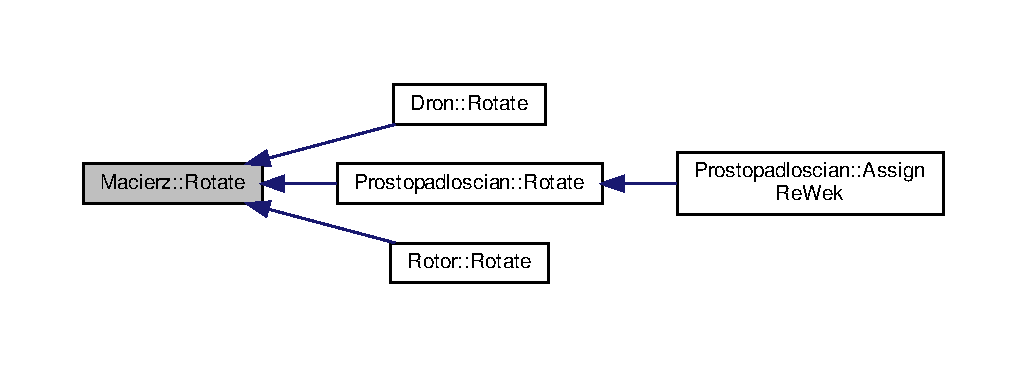
\includegraphics[width=350pt]{class_macierz_ad7d0f072e450b04740723cfa7b13af17_icgraph}
\end{center}
\end{figure}


The documentation for this class was generated from the following file\+:\begin{DoxyCompactItemize}
\item 
inc/\hyperlink{_macierz_8hh}{Macierz.\+hh}\end{DoxyCompactItemize}

\hypertarget{class_obj___geo}{}\section{Obj\+\_\+\+Geo Class Reference}
\label{class_obj___geo}\index{Obj\+\_\+\+Geo@{Obj\+\_\+\+Geo}}


{\ttfamily \#include $<$Obj\+\_\+\+Geo.\+hh$>$}



Inheritance diagram for Obj\+\_\+\+Geo\+:
\nopagebreak
\begin{figure}[H]
\begin{center}
\leavevmode
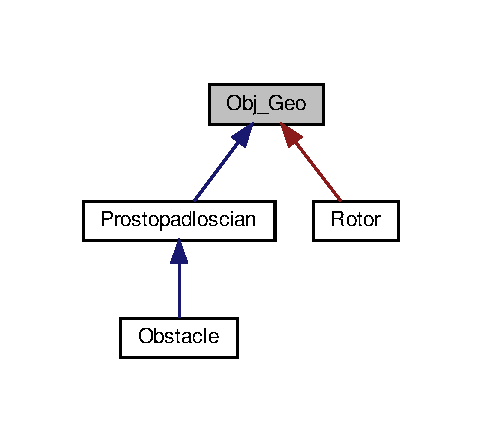
\includegraphics[width=232pt]{class_obj___geo__inherit__graph}
\end{center}
\end{figure}
\subsection*{Public Attributes}
\begin{DoxyCompactItemize}
\item 
vector$<$ \hyperlink{_wektor3_d_8hh_ac353a272b38b4ad342f7181ad7bdb91a}{Wektor3D} $>$ \hyperlink{class_obj___geo_a3f4f092908f6269abc82a9ead4e1565b}{Vector}
\end{DoxyCompactItemize}


\subsection{Detailed Description}


Definition at line 10 of file Obj\+\_\+\+Geo.\+hh.



\subsection{Member Data Documentation}
\mbox{\Hypertarget{class_obj___geo_a3f4f092908f6269abc82a9ead4e1565b}\label{class_obj___geo_a3f4f092908f6269abc82a9ead4e1565b}} 
\index{Obj\+\_\+\+Geo@{Obj\+\_\+\+Geo}!Vector@{Vector}}
\index{Vector@{Vector}!Obj\+\_\+\+Geo@{Obj\+\_\+\+Geo}}
\subsubsection{\texorpdfstring{Vector}{Vector}}
{\footnotesize\ttfamily vector$<$\hyperlink{_wektor3_d_8hh_ac353a272b38b4ad342f7181ad7bdb91a}{Wektor3D}$>$ Obj\+\_\+\+Geo\+::\+Vector}



Definition at line 12 of file Obj\+\_\+\+Geo.\+hh.



The documentation for this class was generated from the following file\+:\begin{DoxyCompactItemize}
\item 
inc/\hyperlink{_obj___geo_8hh}{Obj\+\_\+\+Geo.\+hh}\end{DoxyCompactItemize}

\hypertarget{class_obj___sc}{}\section{Obj\+\_\+\+Sc Class Reference}
\label{class_obj___sc}\index{Obj\+\_\+\+Sc@{Obj\+\_\+\+Sc}}


Klasa ta jest dziedziczona do drona oraz przeszkody. Jego metodą jest wykrywanie kolizji.  




{\ttfamily \#include $<$Obj\+\_\+\+Sc.\+hh$>$}



Inheritance diagram for Obj\+\_\+\+Sc\+:
\nopagebreak
\begin{figure}[H]
\begin{center}
\leavevmode
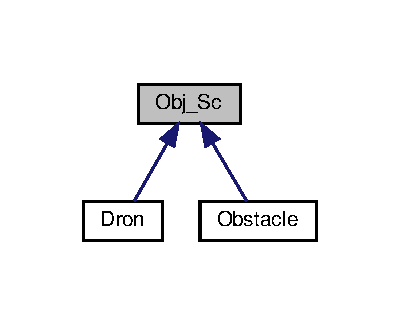
\includegraphics[width=192pt]{class_obj___sc__inherit__graph}
\end{center}
\end{figure}
\subsection*{Public Member Functions}
\begin{DoxyCompactItemize}
\item 
bool \hyperlink{class_obj___sc_ab908a242bc8ba6a409477314f23ce2d6}{Is\+Colision} (\hyperlink{class_obj___sc}{Obj\+\_\+\+Sc} \&OS, double \&d)
\end{DoxyCompactItemize}


\subsection{Detailed Description}
Klasa ta jest dziedziczona do drona oraz przeszkody. Jego metodą jest wykrywanie kolizji. 

Definition at line 13 of file Obj\+\_\+\+Sc.\+hh.



\subsection{Member Function Documentation}
\mbox{\Hypertarget{class_obj___sc_ab908a242bc8ba6a409477314f23ce2d6}\label{class_obj___sc_ab908a242bc8ba6a409477314f23ce2d6}} 
\index{Obj\+\_\+\+Sc@{Obj\+\_\+\+Sc}!Is\+Colision@{Is\+Colision}}
\index{Is\+Colision@{Is\+Colision}!Obj\+\_\+\+Sc@{Obj\+\_\+\+Sc}}
\subsubsection{\texorpdfstring{Is\+Colision()}{IsColision()}}
{\footnotesize\ttfamily bool Obj\+\_\+\+Sc\+::\+Is\+Colision (\begin{DoxyParamCaption}\item[{\hyperlink{class_obj___sc}{Obj\+\_\+\+Sc} \&}]{OS,  }\item[{double \&}]{d }\end{DoxyParamCaption})}



The documentation for this class was generated from the following file\+:\begin{DoxyCompactItemize}
\item 
inc/\hyperlink{_obj___sc_8hh}{Obj\+\_\+\+Sc.\+hh}\end{DoxyCompactItemize}

\hypertarget{class_obstacle}{}\section{Obstacle Class Reference}
\label{class_obstacle}\index{Obstacle@{Obstacle}}


Klasa określa przeszkode. Jest fragmentem objektu sceny.  




{\ttfamily \#include $<$Obstacle.\+hh$>$}



Inheritance diagram for Obstacle\+:
\nopagebreak
\begin{figure}[H]
\begin{center}
\leavevmode
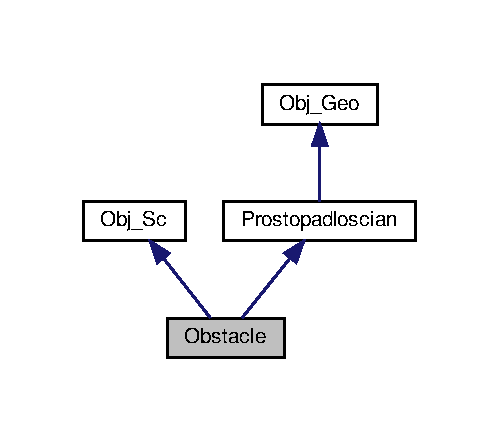
\includegraphics[width=240pt]{class_obstacle__inherit__graph}
\end{center}
\end{figure}


Collaboration diagram for Obstacle\+:
\nopagebreak
\begin{figure}[H]
\begin{center}
\leavevmode
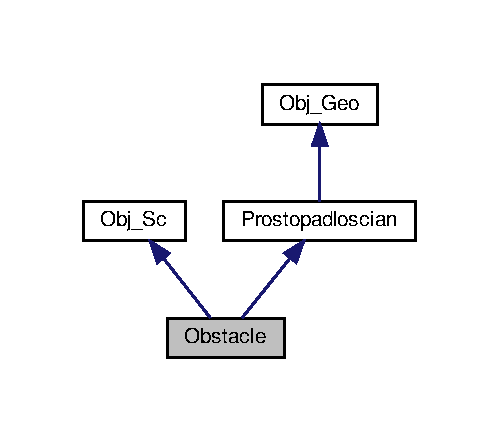
\includegraphics[width=240pt]{class_obstacle__coll__graph}
\end{center}
\end{figure}
\subsection*{Additional Inherited Members}


\subsection{Detailed Description}
Klasa określa przeszkode. Jest fragmentem objektu sceny. 

Definition at line 14 of file Obstacle.\+hh.



The documentation for this class was generated from the following file\+:\begin{DoxyCompactItemize}
\item 
inc/\hyperlink{_obstacle_8hh}{Obstacle.\+hh}\end{DoxyCompactItemize}

\hypertarget{class_prostopadloscian}{}\section{Prostopadloscian Class Reference}
\label{class_prostopadloscian}\index{Prostopadloscian@{Prostopadloscian}}


Klasa ta reprezentuje prostopadłościan oraz to co go określa (współrzędne, metody obrotu, translacji itp).  




{\ttfamily \#include $<$Prostopadloscian.\+hh$>$}



Inheritance diagram for Prostopadloscian\+:
\nopagebreak
\begin{figure}[H]
\begin{center}
\leavevmode
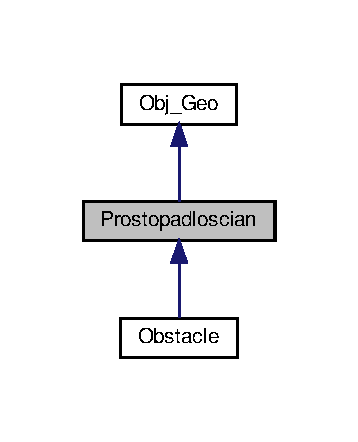
\includegraphics[width=172pt]{class_prostopadloscian__inherit__graph}
\end{center}
\end{figure}


Collaboration diagram for Prostopadloscian\+:
\nopagebreak
\begin{figure}[H]
\begin{center}
\leavevmode
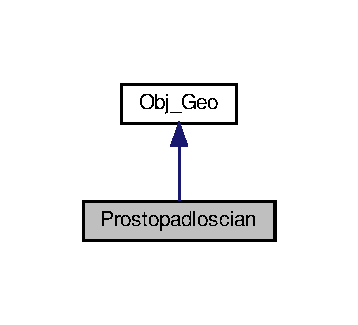
\includegraphics[width=172pt]{class_prostopadloscian__coll__graph}
\end{center}
\end{figure}
\subsection*{Public Member Functions}
\begin{DoxyCompactItemize}
\item 
int \hyperlink{class_prostopadloscian_ac06bcf13d7548f9787d72b88512bf013}{Re\+Angle1} (\hyperlink{class_prostopadloscian}{Prostopadloscian} \&P, int kat)
\item 
int \hyperlink{class_prostopadloscian_a13ac6e1d2da93164f16552be60055049}{Re\+Angle2} (\hyperlink{class_prostopadloscian}{Prostopadloscian} \&P)
\item 
\hyperlink{_wektor3_d_8hh_ac353a272b38b4ad342f7181ad7bdb91a}{Wektor3D} \hyperlink{class_prostopadloscian_ae7f0619842a6b21eeb7873c85f20cdf9}{Re\+Trans1} (\hyperlink{class_prostopadloscian}{Prostopadloscian} \&P, \hyperlink{_wektor3_d_8hh_ac353a272b38b4ad342f7181ad7bdb91a}{Wektor3D} Ve)
\item 
\hyperlink{_wektor3_d_8hh_ac353a272b38b4ad342f7181ad7bdb91a}{Wektor3D} \hyperlink{class_prostopadloscian_af6d4709d4c10a07a96147450ab3d29e8}{Re\+Trans2} (\hyperlink{class_prostopadloscian}{Prostopadloscian} \&P)
\item 
void \hyperlink{class_prostopadloscian_a98ee1de208d5a2ce4b40d88841498a66}{Assign\+Re\+Wek} ()
\item 
void \hyperlink{class_prostopadloscian_a3c00c5ac04367876833db20981e36a68}{Rotate} (\hyperlink{class_prostopadloscian}{Prostopadloscian} \&Pr, int kat)
\item 
void \hyperlink{class_prostopadloscian_a4b5870cc10216feaf8a23e8f9088e3ac}{Translate} (\hyperlink{class_prostopadloscian}{Prostopadloscian} \&Pr, \hyperlink{_wektor3_d_8hh_ac353a272b38b4ad342f7181ad7bdb91a}{Wektor3D} V)
\item 
\hyperlink{_wektor3_d_8hh_ac353a272b38b4ad342f7181ad7bdb91a}{Wektor3D} \hyperlink{class_prostopadloscian_af2117035517518b659795c49948c8836}{operator\mbox{[}$\,$\mbox{]}} (int ind) const
\item 
void \hyperlink{class_prostopadloscian_a42c4460d389ab1a0b62b6cf3e84abccd}{Push\+Back} (\hyperlink{_wektor3_d_8hh_ac353a272b38b4ad342f7181ad7bdb91a}{Wektor3D} VV)
\item 
\hyperlink{_wektor3_d_8hh_ac353a272b38b4ad342f7181ad7bdb91a}{Wektor3D} \& \hyperlink{class_prostopadloscian_a84dc465ece10f2fa7d60e64fc70f29c6}{operator\mbox{[}$\,$\mbox{]}} (int ind)
\end{DoxyCompactItemize}
\subsection*{Additional Inherited Members}


\subsection{Detailed Description}
Klasa ta reprezentuje prostopadłościan oraz to co go określa (współrzędne, metody obrotu, translacji itp). 

Definition at line 9 of file Prostopadloscian.\+hh.



\subsection{Member Function Documentation}
\mbox{\Hypertarget{class_prostopadloscian_a98ee1de208d5a2ce4b40d88841498a66}\label{class_prostopadloscian_a98ee1de208d5a2ce4b40d88841498a66}} 
\index{Prostopadloscian@{Prostopadloscian}!Assign\+Re\+Wek@{Assign\+Re\+Wek}}
\index{Assign\+Re\+Wek@{Assign\+Re\+Wek}!Prostopadloscian@{Prostopadloscian}}
\subsubsection{\texorpdfstring{Assign\+Re\+Wek()}{AssignReWek()}}
{\footnotesize\ttfamily void Prostopadloscian\+::\+Assign\+Re\+Wek (\begin{DoxyParamCaption}{ }\end{DoxyParamCaption})\hspace{0.3cm}{\ttfamily [inline]}}



Definition at line 20 of file Prostopadloscian.\+hh.

Here is the call graph for this function\+:
\nopagebreak
\begin{figure}[H]
\begin{center}
\leavevmode
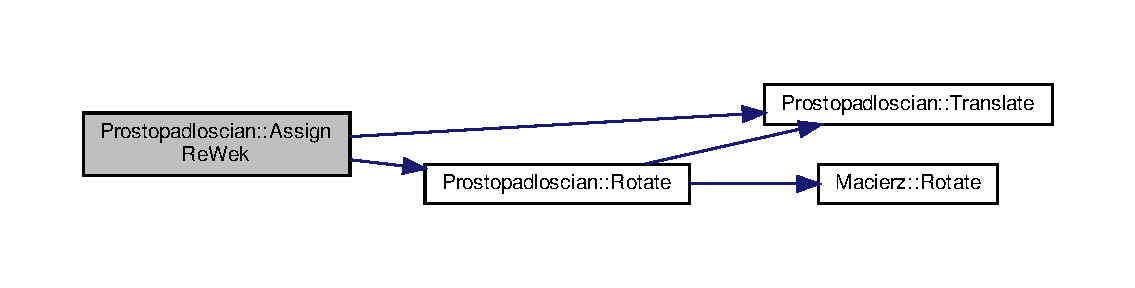
\includegraphics[width=350pt]{class_prostopadloscian_a98ee1de208d5a2ce4b40d88841498a66_cgraph}
\end{center}
\end{figure}
\mbox{\Hypertarget{class_prostopadloscian_af2117035517518b659795c49948c8836}\label{class_prostopadloscian_af2117035517518b659795c49948c8836}} 
\index{Prostopadloscian@{Prostopadloscian}!operator\mbox{[}\mbox{]}@{operator[]}}
\index{operator\mbox{[}\mbox{]}@{operator[]}!Prostopadloscian@{Prostopadloscian}}
\subsubsection{\texorpdfstring{operator[]()}{operator[]()}\hspace{0.1cm}{\footnotesize\ttfamily [1/2]}}
{\footnotesize\ttfamily \hyperlink{_wektor3_d_8hh_ac353a272b38b4ad342f7181ad7bdb91a}{Wektor3D} Prostopadloscian\+::operator\mbox{[}$\,$\mbox{]} (\begin{DoxyParamCaption}\item[{int}]{ind }\end{DoxyParamCaption}) const\hspace{0.3cm}{\ttfamily [inline]}}



Definition at line 29 of file Prostopadloscian.\+hh.

\mbox{\Hypertarget{class_prostopadloscian_a84dc465ece10f2fa7d60e64fc70f29c6}\label{class_prostopadloscian_a84dc465ece10f2fa7d60e64fc70f29c6}} 
\index{Prostopadloscian@{Prostopadloscian}!operator\mbox{[}\mbox{]}@{operator[]}}
\index{operator\mbox{[}\mbox{]}@{operator[]}!Prostopadloscian@{Prostopadloscian}}
\subsubsection{\texorpdfstring{operator[]()}{operator[]()}\hspace{0.1cm}{\footnotesize\ttfamily [2/2]}}
{\footnotesize\ttfamily \hyperlink{_wektor3_d_8hh_ac353a272b38b4ad342f7181ad7bdb91a}{Wektor3D}\& Prostopadloscian\+::operator\mbox{[}$\,$\mbox{]} (\begin{DoxyParamCaption}\item[{int}]{ind }\end{DoxyParamCaption})\hspace{0.3cm}{\ttfamily [inline]}}



Definition at line 31 of file Prostopadloscian.\+hh.

Here is the call graph for this function\+:
\nopagebreak
\begin{figure}[H]
\begin{center}
\leavevmode
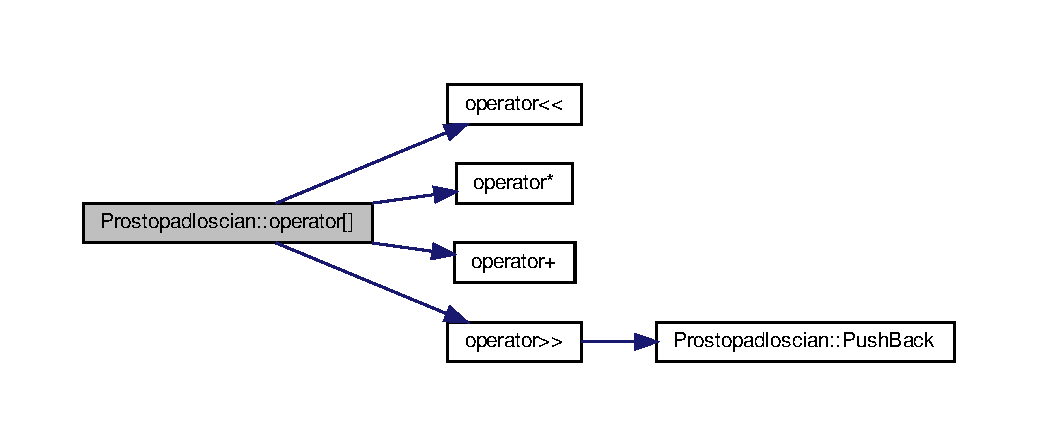
\includegraphics[width=350pt]{class_prostopadloscian_a84dc465ece10f2fa7d60e64fc70f29c6_cgraph}
\end{center}
\end{figure}
\mbox{\Hypertarget{class_prostopadloscian_a42c4460d389ab1a0b62b6cf3e84abccd}\label{class_prostopadloscian_a42c4460d389ab1a0b62b6cf3e84abccd}} 
\index{Prostopadloscian@{Prostopadloscian}!Push\+Back@{Push\+Back}}
\index{Push\+Back@{Push\+Back}!Prostopadloscian@{Prostopadloscian}}
\subsubsection{\texorpdfstring{Push\+Back()}{PushBack()}}
{\footnotesize\ttfamily void Prostopadloscian\+::\+Push\+Back (\begin{DoxyParamCaption}\item[{\hyperlink{_wektor3_d_8hh_ac353a272b38b4ad342f7181ad7bdb91a}{Wektor3D}}]{VV }\end{DoxyParamCaption})\hspace{0.3cm}{\ttfamily [inline]}}



Definition at line 30 of file Prostopadloscian.\+hh.

Here is the caller graph for this function\+:
\nopagebreak
\begin{figure}[H]
\begin{center}
\leavevmode
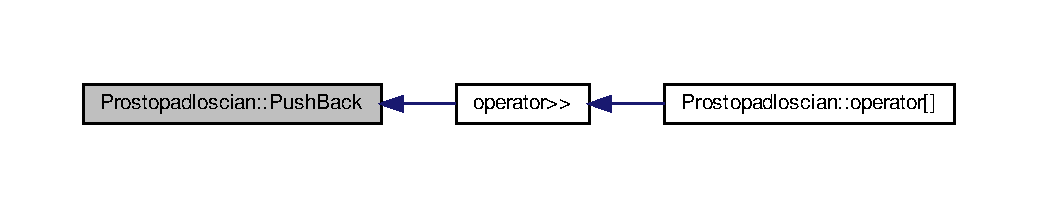
\includegraphics[width=350pt]{class_prostopadloscian_a42c4460d389ab1a0b62b6cf3e84abccd_icgraph}
\end{center}
\end{figure}
\mbox{\Hypertarget{class_prostopadloscian_ac06bcf13d7548f9787d72b88512bf013}\label{class_prostopadloscian_ac06bcf13d7548f9787d72b88512bf013}} 
\index{Prostopadloscian@{Prostopadloscian}!Re\+Angle1@{Re\+Angle1}}
\index{Re\+Angle1@{Re\+Angle1}!Prostopadloscian@{Prostopadloscian}}
\subsubsection{\texorpdfstring{Re\+Angle1()}{ReAngle1()}}
{\footnotesize\ttfamily int Prostopadloscian\+::\+Re\+Angle1 (\begin{DoxyParamCaption}\item[{\hyperlink{class_prostopadloscian}{Prostopadloscian} \&}]{P,  }\item[{int}]{kat }\end{DoxyParamCaption})}



Definition at line 6 of file Prostopadloscian.\+cpp.

\mbox{\Hypertarget{class_prostopadloscian_a13ac6e1d2da93164f16552be60055049}\label{class_prostopadloscian_a13ac6e1d2da93164f16552be60055049}} 
\index{Prostopadloscian@{Prostopadloscian}!Re\+Angle2@{Re\+Angle2}}
\index{Re\+Angle2@{Re\+Angle2}!Prostopadloscian@{Prostopadloscian}}
\subsubsection{\texorpdfstring{Re\+Angle2()}{ReAngle2()}}
{\footnotesize\ttfamily int Prostopadloscian\+::\+Re\+Angle2 (\begin{DoxyParamCaption}\item[{\hyperlink{class_prostopadloscian}{Prostopadloscian} \&}]{P }\end{DoxyParamCaption})}



Definition at line 11 of file Prostopadloscian.\+cpp.

\mbox{\Hypertarget{class_prostopadloscian_ae7f0619842a6b21eeb7873c85f20cdf9}\label{class_prostopadloscian_ae7f0619842a6b21eeb7873c85f20cdf9}} 
\index{Prostopadloscian@{Prostopadloscian}!Re\+Trans1@{Re\+Trans1}}
\index{Re\+Trans1@{Re\+Trans1}!Prostopadloscian@{Prostopadloscian}}
\subsubsection{\texorpdfstring{Re\+Trans1()}{ReTrans1()}}
{\footnotesize\ttfamily \hyperlink{_wektor3_d_8hh_ac353a272b38b4ad342f7181ad7bdb91a}{Wektor3D} Prostopadloscian\+::\+Re\+Trans1 (\begin{DoxyParamCaption}\item[{\hyperlink{class_prostopadloscian}{Prostopadloscian} \&}]{P,  }\item[{\hyperlink{_wektor3_d_8hh_ac353a272b38b4ad342f7181ad7bdb91a}{Wektor3D}}]{Ve }\end{DoxyParamCaption})}



Definition at line 16 of file Prostopadloscian.\+cpp.

\mbox{\Hypertarget{class_prostopadloscian_af6d4709d4c10a07a96147450ab3d29e8}\label{class_prostopadloscian_af6d4709d4c10a07a96147450ab3d29e8}} 
\index{Prostopadloscian@{Prostopadloscian}!Re\+Trans2@{Re\+Trans2}}
\index{Re\+Trans2@{Re\+Trans2}!Prostopadloscian@{Prostopadloscian}}
\subsubsection{\texorpdfstring{Re\+Trans2()}{ReTrans2()}}
{\footnotesize\ttfamily \hyperlink{_wektor3_d_8hh_ac353a272b38b4ad342f7181ad7bdb91a}{Wektor3D} Prostopadloscian\+::\+Re\+Trans2 (\begin{DoxyParamCaption}\item[{\hyperlink{class_prostopadloscian}{Prostopadloscian} \&}]{P }\end{DoxyParamCaption})}



Definition at line 21 of file Prostopadloscian.\+cpp.

\mbox{\Hypertarget{class_prostopadloscian_a3c00c5ac04367876833db20981e36a68}\label{class_prostopadloscian_a3c00c5ac04367876833db20981e36a68}} 
\index{Prostopadloscian@{Prostopadloscian}!Rotate@{Rotate}}
\index{Rotate@{Rotate}!Prostopadloscian@{Prostopadloscian}}
\subsubsection{\texorpdfstring{Rotate()}{Rotate()}}
{\footnotesize\ttfamily void Prostopadloscian\+::\+Rotate (\begin{DoxyParamCaption}\item[{\hyperlink{class_prostopadloscian}{Prostopadloscian} \&}]{Pr,  }\item[{int}]{kat }\end{DoxyParamCaption})}

Obraca prostopadłościan o zadany kąt 

Definition at line 26 of file Prostopadloscian.\+cpp.

Here is the call graph for this function\+:
\nopagebreak
\begin{figure}[H]
\begin{center}
\leavevmode
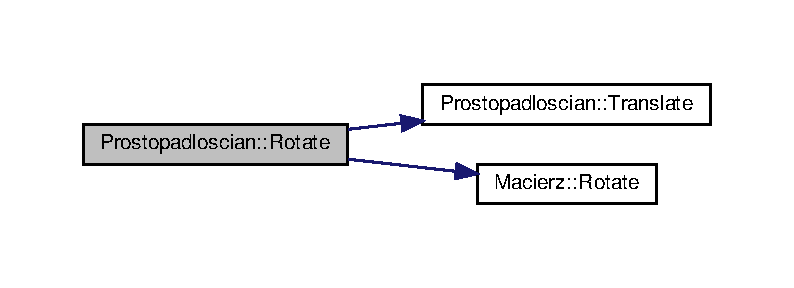
\includegraphics[width=350pt]{class_prostopadloscian_a3c00c5ac04367876833db20981e36a68_cgraph}
\end{center}
\end{figure}
Here is the caller graph for this function\+:
\nopagebreak
\begin{figure}[H]
\begin{center}
\leavevmode
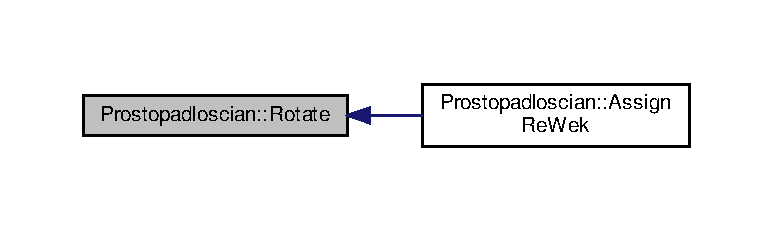
\includegraphics[width=350pt]{class_prostopadloscian_a3c00c5ac04367876833db20981e36a68_icgraph}
\end{center}
\end{figure}
\mbox{\Hypertarget{class_prostopadloscian_a4b5870cc10216feaf8a23e8f9088e3ac}\label{class_prostopadloscian_a4b5870cc10216feaf8a23e8f9088e3ac}} 
\index{Prostopadloscian@{Prostopadloscian}!Translate@{Translate}}
\index{Translate@{Translate}!Prostopadloscian@{Prostopadloscian}}
\subsubsection{\texorpdfstring{Translate()}{Translate()}}
{\footnotesize\ttfamily void Prostopadloscian\+::\+Translate (\begin{DoxyParamCaption}\item[{\hyperlink{class_prostopadloscian}{Prostopadloscian} \&}]{Pr,  }\item[{\hyperlink{_wektor3_d_8hh_ac353a272b38b4ad342f7181ad7bdb91a}{Wektor3D}}]{V }\end{DoxyParamCaption})}

Wykonuje translacje o zadany wektor 

Definition at line 39 of file Prostopadloscian.\+cpp.

Here is the caller graph for this function\+:
\nopagebreak
\begin{figure}[H]
\begin{center}
\leavevmode
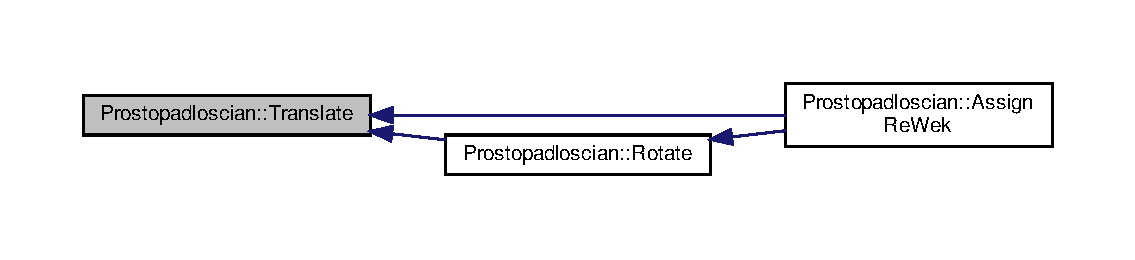
\includegraphics[width=350pt]{class_prostopadloscian_a4b5870cc10216feaf8a23e8f9088e3ac_icgraph}
\end{center}
\end{figure}


The documentation for this class was generated from the following files\+:\begin{DoxyCompactItemize}
\item 
inc/\hyperlink{_prostopadloscian_8hh}{Prostopadloscian.\+hh}\item 
src/\hyperlink{_prostopadloscian_8cpp}{Prostopadloscian.\+cpp}\end{DoxyCompactItemize}

\hypertarget{class_rotor}{}\section{Rotor Class Reference}
\label{class_rotor}\index{Rotor@{Rotor}}


Klasa określa współrzędne rotorów oraz jak się obracają  




{\ttfamily \#include $<$Rotor.\+hh$>$}



Inheritance diagram for Rotor\+:
\nopagebreak
\begin{figure}[H]
\begin{center}
\leavevmode
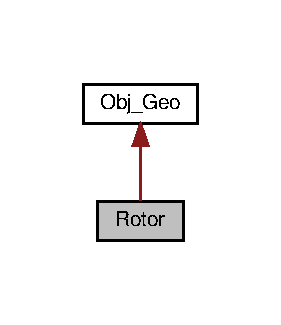
\includegraphics[width=135pt]{class_rotor__inherit__graph}
\end{center}
\end{figure}


Collaboration diagram for Rotor\+:
\nopagebreak
\begin{figure}[H]
\begin{center}
\leavevmode
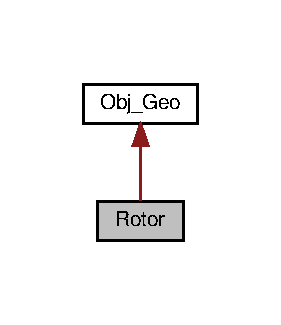
\includegraphics[width=135pt]{class_rotor__coll__graph}
\end{center}
\end{figure}
\subsection*{Public Member Functions}
\begin{DoxyCompactItemize}
\item 
void \hyperlink{class_rotor_a021ab148b8734f0a82d502c999dd41be}{Rotate} (\hyperlink{class_rotor}{Rotor} \&R, int kat)
\item 
void \hyperlink{class_rotor_a1f00a40e0e40e8f8cf7cb15160c88cc2}{Translate} (\hyperlink{class_rotor}{Rotor} \&R, \hyperlink{_wektor3_d_8hh_ac353a272b38b4ad342f7181ad7bdb91a}{Wektor3D} V)
\item 
\hyperlink{_wektor3_d_8hh_ac353a272b38b4ad342f7181ad7bdb91a}{Wektor3D} \hyperlink{class_rotor_a10b8d092c1604fbef24ee2c5977c26ae}{operator()} (int ind) const
\item 
void \hyperlink{class_rotor_a987eda3f97cef17d1201057078185ad6}{Push\+Back} (\hyperlink{_wektor3_d_8hh_ac353a272b38b4ad342f7181ad7bdb91a}{Wektor3D} VV)
\item 
\hyperlink{_wektor3_d_8hh_ac353a272b38b4ad342f7181ad7bdb91a}{Wektor3D} \& \hyperlink{class_rotor_ad43dd1c9b8def16cdbae6b12b4968f23}{operator()} (int ind)
\end{DoxyCompactItemize}


\subsection{Detailed Description}
Klasa określa współrzędne rotorów oraz jak się obracają 

Definition at line 15 of file Rotor.\+hh.



\subsection{Member Function Documentation}
\mbox{\Hypertarget{class_rotor_a10b8d092c1604fbef24ee2c5977c26ae}\label{class_rotor_a10b8d092c1604fbef24ee2c5977c26ae}} 
\index{Rotor@{Rotor}!operator()@{operator()}}
\index{operator()@{operator()}!Rotor@{Rotor}}
\subsubsection{\texorpdfstring{operator()()}{operator()()}\hspace{0.1cm}{\footnotesize\ttfamily [1/2]}}
{\footnotesize\ttfamily \hyperlink{_wektor3_d_8hh_ac353a272b38b4ad342f7181ad7bdb91a}{Wektor3D} Rotor\+::operator() (\begin{DoxyParamCaption}\item[{int}]{ind }\end{DoxyParamCaption}) const\hspace{0.3cm}{\ttfamily [inline]}}



Definition at line 23 of file Rotor.\+hh.

\mbox{\Hypertarget{class_rotor_ad43dd1c9b8def16cdbae6b12b4968f23}\label{class_rotor_ad43dd1c9b8def16cdbae6b12b4968f23}} 
\index{Rotor@{Rotor}!operator()@{operator()}}
\index{operator()@{operator()}!Rotor@{Rotor}}
\subsubsection{\texorpdfstring{operator()()}{operator()()}\hspace{0.1cm}{\footnotesize\ttfamily [2/2]}}
{\footnotesize\ttfamily \hyperlink{_wektor3_d_8hh_ac353a272b38b4ad342f7181ad7bdb91a}{Wektor3D}\& Rotor\+::operator() (\begin{DoxyParamCaption}\item[{int}]{ind }\end{DoxyParamCaption})\hspace{0.3cm}{\ttfamily [inline]}}



Definition at line 25 of file Rotor.\+hh.

Here is the call graph for this function\+:
\nopagebreak
\begin{figure}[H]
\begin{center}
\leavevmode
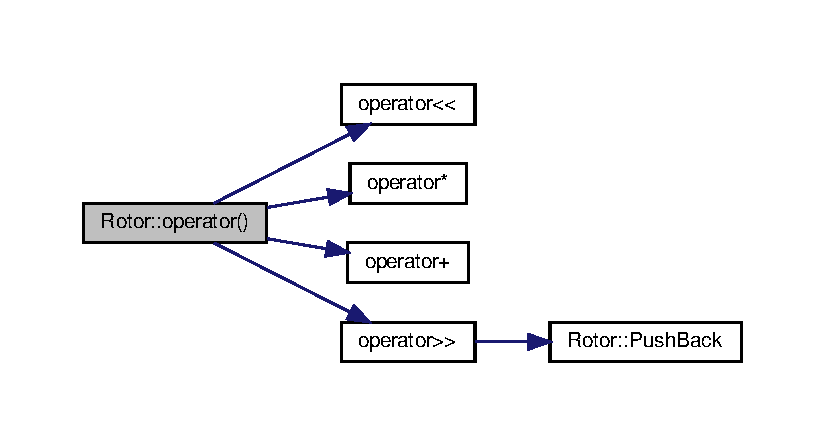
\includegraphics[width=350pt]{class_rotor_ad43dd1c9b8def16cdbae6b12b4968f23_cgraph}
\end{center}
\end{figure}
\mbox{\Hypertarget{class_rotor_a987eda3f97cef17d1201057078185ad6}\label{class_rotor_a987eda3f97cef17d1201057078185ad6}} 
\index{Rotor@{Rotor}!Push\+Back@{Push\+Back}}
\index{Push\+Back@{Push\+Back}!Rotor@{Rotor}}
\subsubsection{\texorpdfstring{Push\+Back()}{PushBack()}}
{\footnotesize\ttfamily void Rotor\+::\+Push\+Back (\begin{DoxyParamCaption}\item[{\hyperlink{_wektor3_d_8hh_ac353a272b38b4ad342f7181ad7bdb91a}{Wektor3D}}]{VV }\end{DoxyParamCaption})\hspace{0.3cm}{\ttfamily [inline]}}



Definition at line 24 of file Rotor.\+hh.

Here is the caller graph for this function\+:
\nopagebreak
\begin{figure}[H]
\begin{center}
\leavevmode
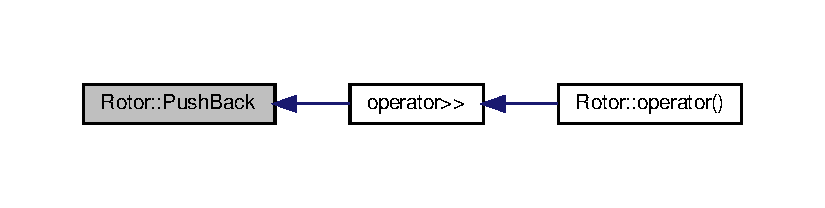
\includegraphics[width=350pt]{class_rotor_a987eda3f97cef17d1201057078185ad6_icgraph}
\end{center}
\end{figure}
\mbox{\Hypertarget{class_rotor_a021ab148b8734f0a82d502c999dd41be}\label{class_rotor_a021ab148b8734f0a82d502c999dd41be}} 
\index{Rotor@{Rotor}!Rotate@{Rotate}}
\index{Rotate@{Rotate}!Rotor@{Rotor}}
\subsubsection{\texorpdfstring{Rotate()}{Rotate()}}
{\footnotesize\ttfamily void Rotor\+::\+Rotate (\begin{DoxyParamCaption}\item[{\hyperlink{class_rotor}{Rotor} \&}]{R,  }\item[{int}]{kat }\end{DoxyParamCaption})}

Obraca prostopadłościan o zadany kąt 

Definition at line 7 of file Rotor.\+cpp.

Here is the call graph for this function\+:
\nopagebreak
\begin{figure}[H]
\begin{center}
\leavevmode
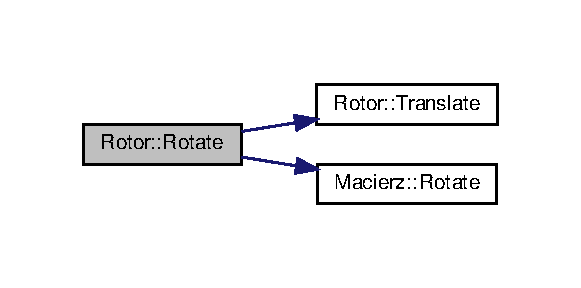
\includegraphics[width=279pt]{class_rotor_a021ab148b8734f0a82d502c999dd41be_cgraph}
\end{center}
\end{figure}
\mbox{\Hypertarget{class_rotor_a1f00a40e0e40e8f8cf7cb15160c88cc2}\label{class_rotor_a1f00a40e0e40e8f8cf7cb15160c88cc2}} 
\index{Rotor@{Rotor}!Translate@{Translate}}
\index{Translate@{Translate}!Rotor@{Rotor}}
\subsubsection{\texorpdfstring{Translate()}{Translate()}}
{\footnotesize\ttfamily void Rotor\+::\+Translate (\begin{DoxyParamCaption}\item[{\hyperlink{class_rotor}{Rotor} \&}]{R,  }\item[{\hyperlink{_wektor3_d_8hh_ac353a272b38b4ad342f7181ad7bdb91a}{Wektor3D}}]{V }\end{DoxyParamCaption})}

Wykonuje translacje o zadany wektor 

Definition at line 21 of file Rotor.\+cpp.

Here is the caller graph for this function\+:
\nopagebreak
\begin{figure}[H]
\begin{center}
\leavevmode
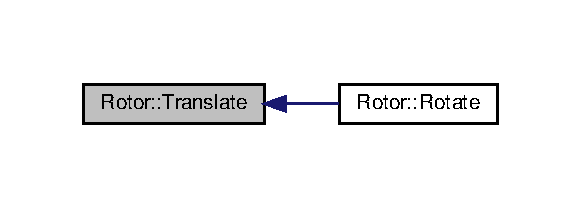
\includegraphics[width=279pt]{class_rotor_a1f00a40e0e40e8f8cf7cb15160c88cc2_icgraph}
\end{center}
\end{figure}


The documentation for this class was generated from the following files\+:\begin{DoxyCompactItemize}
\item 
inc/\hyperlink{_rotor_8hh}{Rotor.\+hh}\item 
src/\hyperlink{_rotor_8cpp}{Rotor.\+cpp}\end{DoxyCompactItemize}

\hypertarget{class_scena}{}\section{Scena Class Reference}
\label{class_scena}\index{Scena@{Scena}}


Klasa ta reprezentuje scene. Jego polami to lista objektów scen oraz dronów.  




{\ttfamily \#include $<$Scena.\+hh$>$}

\subsection*{Public Member Functions}
\begin{DoxyCompactItemize}
\item 
void \hyperlink{class_scena_a058812f85dc08a6e4b66f38028393d64}{D\+Push\+Back} (shared\+\_\+ptr$<$ \hyperlink{class_dron}{Dron} $>$ \&D)
\item 
void \hyperlink{class_scena_adf77e0e73d6bc9aa0c8b0a27225aaa14}{O\+Push\+Back} (shared\+\_\+ptr$<$ \hyperlink{class_obj___sc}{Obj\+\_\+\+Sc} $>$ O)
\end{DoxyCompactItemize}


\subsection{Detailed Description}
Klasa ta reprezentuje scene. Jego polami to lista objektów scen oraz dronów. 

Definition at line 13 of file Scena.\+hh.



\subsection{Member Function Documentation}
\mbox{\Hypertarget{class_scena_a058812f85dc08a6e4b66f38028393d64}\label{class_scena_a058812f85dc08a6e4b66f38028393d64}} 
\index{Scena@{Scena}!D\+Push\+Back@{D\+Push\+Back}}
\index{D\+Push\+Back@{D\+Push\+Back}!Scena@{Scena}}
\subsubsection{\texorpdfstring{D\+Push\+Back()}{DPushBack()}}
{\footnotesize\ttfamily void Scena\+::\+D\+Push\+Back (\begin{DoxyParamCaption}\item[{shared\+\_\+ptr$<$ \hyperlink{class_dron}{Dron} $>$ \&}]{D }\end{DoxyParamCaption})}



Definition at line 12 of file Scena.\+cpp.

\mbox{\Hypertarget{class_scena_adf77e0e73d6bc9aa0c8b0a27225aaa14}\label{class_scena_adf77e0e73d6bc9aa0c8b0a27225aaa14}} 
\index{Scena@{Scena}!O\+Push\+Back@{O\+Push\+Back}}
\index{O\+Push\+Back@{O\+Push\+Back}!Scena@{Scena}}
\subsubsection{\texorpdfstring{O\+Push\+Back()}{OPushBack()}}
{\footnotesize\ttfamily void Scena\+::\+O\+Push\+Back (\begin{DoxyParamCaption}\item[{shared\+\_\+ptr$<$ \hyperlink{class_obj___sc}{Obj\+\_\+\+Sc} $>$}]{O }\end{DoxyParamCaption})}



Definition at line 16 of file Scena.\+cpp.



The documentation for this class was generated from the following files\+:\begin{DoxyCompactItemize}
\item 
inc/\hyperlink{_scena_8hh}{Scena.\+hh}\item 
src/\hyperlink{_scena_8cpp}{Scena.\+cpp}\end{DoxyCompactItemize}

\hypertarget{class_wektor}{}\section{Wektor$<$ Wymiar $>$ Class Template Reference}
\label{class_wektor}\index{Wektor$<$ Wymiar $>$@{Wektor$<$ Wymiar $>$}}


Klasa ta reprezentuje wektor (tablica n-\/wymiarowa, przeciążenia operatorów itp).  




{\ttfamily \#include $<$Wektor.\+hh$>$}

\subsection*{Public Member Functions}
\begin{DoxyCompactItemize}
\item 
\hyperlink{class_wektor_acfa7e8deeb9dacb94d3c3d13b1f23d8f}{Wektor} ()
\item 
\hyperlink{class_wektor_a08017a99d115b17957e728d5ac2dc432}{$\sim$\+Wektor} ()
\item 
\hyperlink{class_wektor_a59c95ec1db1b090e29c5cd867953929a}{Wektor} (const \hyperlink{class_wektor}{Wektor} \&obj)
\item 
double \hyperlink{class_wektor_a49964f91d93ff53bd4152665fd93e57d}{Dl\+Wek} ()
\item 
double \hyperlink{class_wektor_a49876d44218344c450fe9e13d9c7e885}{operator\mbox{[}$\,$\mbox{]}} (int ind) const
\item 
double \& \hyperlink{class_wektor_a88d91e6a337390c1e6ab527970c392a4}{operator\mbox{[}$\,$\mbox{]}} (int ind)
\end{DoxyCompactItemize}
\subsection*{Static Public Member Functions}
\begin{DoxyCompactItemize}
\item 
static unsigned int \hyperlink{class_wektor_a438c6da633a43e609467e22b6e2079db}{Show\+Counter} ()
\item 
static unsigned int \hyperlink{class_wektor_a5365d8d93dfaa304c7fbd998e92660b7}{Show\+Sum} ()
\end{DoxyCompactItemize}


\subsection{Detailed Description}
\subsubsection*{template$<$int Wymiar$>$\newline
class Wektor$<$ Wymiar $>$}

Klasa ta reprezentuje wektor (tablica n-\/wymiarowa, przeciążenia operatorów itp). 

Definition at line 10 of file Wektor.\+hh.



\subsection{Constructor \& Destructor Documentation}
\mbox{\Hypertarget{class_wektor_acfa7e8deeb9dacb94d3c3d13b1f23d8f}\label{class_wektor_acfa7e8deeb9dacb94d3c3d13b1f23d8f}} 
\index{Wektor@{Wektor}!Wektor@{Wektor}}
\index{Wektor@{Wektor}!Wektor@{Wektor}}
\subsubsection{\texorpdfstring{Wektor()}{Wektor()}\hspace{0.1cm}{\footnotesize\ttfamily [1/2]}}
{\footnotesize\ttfamily template$<$int Wymiar$>$ \\
\hyperlink{class_wektor}{Wektor}$<$ Wymiar $>$\+::\hyperlink{class_wektor}{Wektor} (\begin{DoxyParamCaption}{ }\end{DoxyParamCaption})\hspace{0.3cm}{\ttfamily [inline]}}



Definition at line 19 of file Wektor.\+hh.

\mbox{\Hypertarget{class_wektor_a08017a99d115b17957e728d5ac2dc432}\label{class_wektor_a08017a99d115b17957e728d5ac2dc432}} 
\index{Wektor@{Wektor}!````~Wektor@{$\sim$\+Wektor}}
\index{````~Wektor@{$\sim$\+Wektor}!Wektor@{Wektor}}
\subsubsection{\texorpdfstring{$\sim$\+Wektor()}{~Wektor()}}
{\footnotesize\ttfamily template$<$int Wymiar$>$ \\
\hyperlink{class_wektor}{Wektor}$<$ Wymiar $>$\+::$\sim$\hyperlink{class_wektor}{Wektor} (\begin{DoxyParamCaption}{ }\end{DoxyParamCaption})\hspace{0.3cm}{\ttfamily [inline]}}



Definition at line 20 of file Wektor.\+hh.

\mbox{\Hypertarget{class_wektor_a59c95ec1db1b090e29c5cd867953929a}\label{class_wektor_a59c95ec1db1b090e29c5cd867953929a}} 
\index{Wektor@{Wektor}!Wektor@{Wektor}}
\index{Wektor@{Wektor}!Wektor@{Wektor}}
\subsubsection{\texorpdfstring{Wektor()}{Wektor()}\hspace{0.1cm}{\footnotesize\ttfamily [2/2]}}
{\footnotesize\ttfamily template$<$int Wymiar$>$ \\
\hyperlink{class_wektor}{Wektor}$<$ Wymiar $>$\+::\hyperlink{class_wektor}{Wektor} (\begin{DoxyParamCaption}\item[{const \hyperlink{class_wektor}{Wektor}$<$ Wymiar $>$ \&}]{obj }\end{DoxyParamCaption})\hspace{0.3cm}{\ttfamily [inline]}}



Definition at line 21 of file Wektor.\+hh.



\subsection{Member Function Documentation}
\mbox{\Hypertarget{class_wektor_a49964f91d93ff53bd4152665fd93e57d}\label{class_wektor_a49964f91d93ff53bd4152665fd93e57d}} 
\index{Wektor@{Wektor}!Dl\+Wek@{Dl\+Wek}}
\index{Dl\+Wek@{Dl\+Wek}!Wektor@{Wektor}}
\subsubsection{\texorpdfstring{Dl\+Wek()}{DlWek()}}
{\footnotesize\ttfamily template$<$int Wymiar$>$ \\
double \hyperlink{class_wektor}{Wektor}$<$ Wymiar $>$\+::Dl\+Wek (\begin{DoxyParamCaption}{ }\end{DoxyParamCaption})}

\hyperlink{class_wektor_a49964f91d93ff53bd4152665fd93e57d}{Dl\+Wek()}-\/oblicza długości wektora 

Definition at line 52 of file Wektor.\+hh.

Here is the caller graph for this function\+:
\nopagebreak
\begin{figure}[H]
\begin{center}
\leavevmode
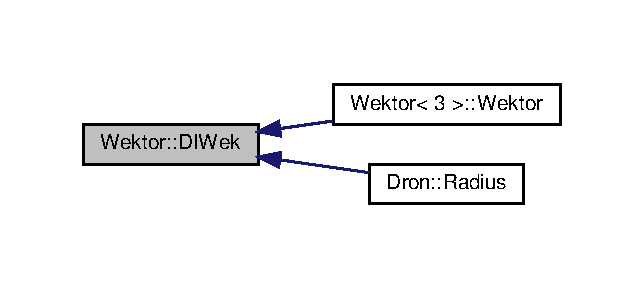
\includegraphics[width=309pt]{class_wektor_a49964f91d93ff53bd4152665fd93e57d_icgraph}
\end{center}
\end{figure}
\mbox{\Hypertarget{class_wektor_a49876d44218344c450fe9e13d9c7e885}\label{class_wektor_a49876d44218344c450fe9e13d9c7e885}} 
\index{Wektor@{Wektor}!operator\mbox{[}\mbox{]}@{operator[]}}
\index{operator\mbox{[}\mbox{]}@{operator[]}!Wektor@{Wektor}}
\subsubsection{\texorpdfstring{operator[]()}{operator[]()}\hspace{0.1cm}{\footnotesize\ttfamily [1/2]}}
{\footnotesize\ttfamily template$<$int Wymiar$>$ \\
double \hyperlink{class_wektor}{Wektor}$<$ Wymiar $>$\+::operator\mbox{[}$\,$\mbox{]} (\begin{DoxyParamCaption}\item[{int}]{ind }\end{DoxyParamCaption}) const\hspace{0.3cm}{\ttfamily [inline]}}



Definition at line 30 of file Wektor.\+hh.

\mbox{\Hypertarget{class_wektor_a88d91e6a337390c1e6ab527970c392a4}\label{class_wektor_a88d91e6a337390c1e6ab527970c392a4}} 
\index{Wektor@{Wektor}!operator\mbox{[}\mbox{]}@{operator[]}}
\index{operator\mbox{[}\mbox{]}@{operator[]}!Wektor@{Wektor}}
\subsubsection{\texorpdfstring{operator[]()}{operator[]()}\hspace{0.1cm}{\footnotesize\ttfamily [2/2]}}
{\footnotesize\ttfamily template$<$int Wymiar$>$ \\
double\& \hyperlink{class_wektor}{Wektor}$<$ Wymiar $>$\+::operator\mbox{[}$\,$\mbox{]} (\begin{DoxyParamCaption}\item[{int}]{ind }\end{DoxyParamCaption})\hspace{0.3cm}{\ttfamily [inline]}}



Definition at line 31 of file Wektor.\+hh.

\mbox{\Hypertarget{class_wektor_a438c6da633a43e609467e22b6e2079db}\label{class_wektor_a438c6da633a43e609467e22b6e2079db}} 
\index{Wektor@{Wektor}!Show\+Counter@{Show\+Counter}}
\index{Show\+Counter@{Show\+Counter}!Wektor@{Wektor}}
\subsubsection{\texorpdfstring{Show\+Counter()}{ShowCounter()}}
{\footnotesize\ttfamily template$<$int Wymiar$>$ \\
unsigned int \hyperlink{class_wektor}{Wektor}$<$ Wymiar $>$\+::Show\+Counter (\begin{DoxyParamCaption}{ }\end{DoxyParamCaption})\hspace{0.3cm}{\ttfamily [static]}}



Definition at line 42 of file Wektor.\+hh.

Here is the caller graph for this function\+:
\nopagebreak
\begin{figure}[H]
\begin{center}
\leavevmode
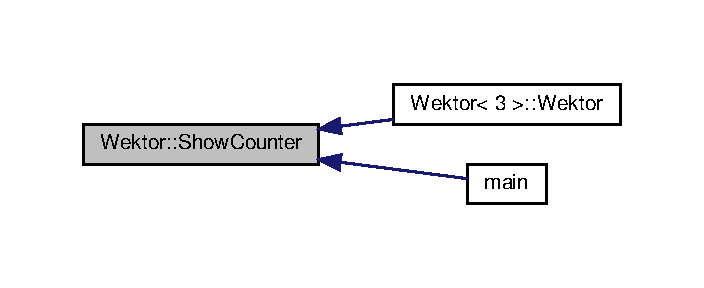
\includegraphics[width=338pt]{class_wektor_a438c6da633a43e609467e22b6e2079db_icgraph}
\end{center}
\end{figure}
\mbox{\Hypertarget{class_wektor_a5365d8d93dfaa304c7fbd998e92660b7}\label{class_wektor_a5365d8d93dfaa304c7fbd998e92660b7}} 
\index{Wektor@{Wektor}!Show\+Sum@{Show\+Sum}}
\index{Show\+Sum@{Show\+Sum}!Wektor@{Wektor}}
\subsubsection{\texorpdfstring{Show\+Sum()}{ShowSum()}}
{\footnotesize\ttfamily template$<$int Wymiar$>$ \\
unsigned int \hyperlink{class_wektor}{Wektor}$<$ Wymiar $>$\+::Show\+Sum (\begin{DoxyParamCaption}{ }\end{DoxyParamCaption})\hspace{0.3cm}{\ttfamily [static]}}



Definition at line 47 of file Wektor.\+hh.

Here is the caller graph for this function\+:
\nopagebreak
\begin{figure}[H]
\begin{center}
\leavevmode
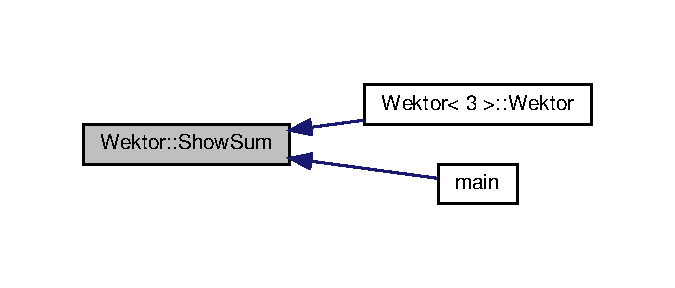
\includegraphics[width=324pt]{class_wektor_a5365d8d93dfaa304c7fbd998e92660b7_icgraph}
\end{center}
\end{figure}


The documentation for this class was generated from the following file\+:\begin{DoxyCompactItemize}
\item 
inc/\hyperlink{_wektor_8hh}{Wektor.\+hh}\end{DoxyCompactItemize}

\chapter{File Documentation}
\hypertarget{_dron_8hh}{}\section{inc/\+Dron.hh File Reference}
\label{_dron_8hh}\index{inc/\+Dron.\+hh@{inc/\+Dron.\+hh}}
{\ttfamily \#include $<$iostream$>$}\newline
{\ttfamily \#include \char`\"{}Prostopadloscian.\+hh\char`\"{}}\newline
{\ttfamily \#include \char`\"{}Rotor.\+hh\char`\"{}}\newline
{\ttfamily \#include \char`\"{}Obj\+\_\+\+Sc.\+hh\char`\"{}}\newline
{\ttfamily \#include $<$memory$>$}\newline
Include dependency graph for Dron.\+hh\+:
\nopagebreak
\begin{figure}[H]
\begin{center}
\leavevmode
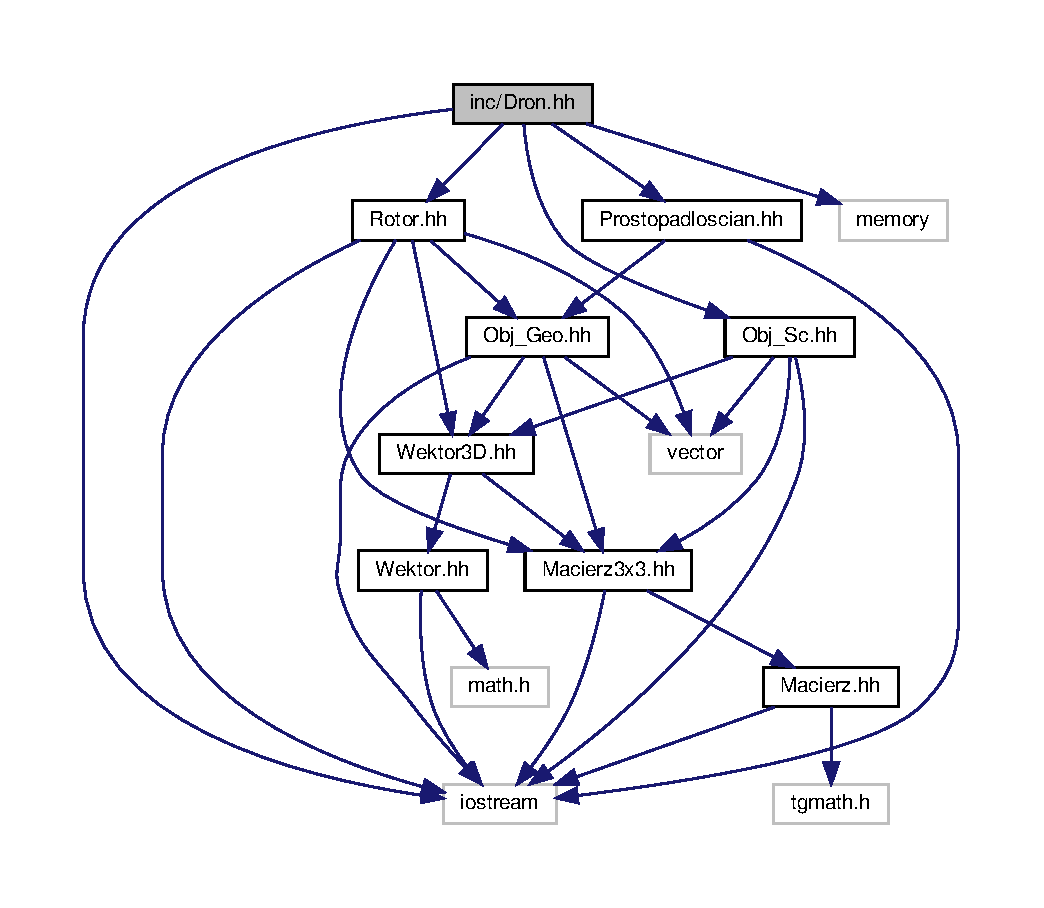
\includegraphics[width=350pt]{_dron_8hh__incl}
\end{center}
\end{figure}
This graph shows which files directly or indirectly include this file\+:
\nopagebreak
\begin{figure}[H]
\begin{center}
\leavevmode
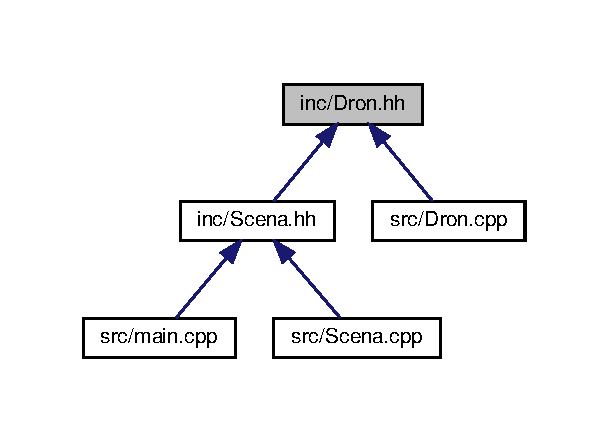
\includegraphics[width=292pt]{_dron_8hh__dep__incl}
\end{center}
\end{figure}
\subsection*{Classes}
\begin{DoxyCompactItemize}
\item 
class \hyperlink{class_dron}{Dron}
\begin{DoxyCompactList}\small\item\em Klasa określa współrzędne rotorów oraz korpusu. Jest fragmentem objektu sceny. \end{DoxyCompactList}\end{DoxyCompactItemize}
\subsection*{Functions}
\begin{DoxyCompactItemize}
\item 
\hyperlink{class_dron}{Dron} \hyperlink{_dron_8hh_a8f9219ec11c21cfdb4178a3ccac3ccc8}{operator$\ast$} (\hyperlink{_macierz3x3_8hh_ad4fc7b0e263d9a99ba6174f68b52ea87}{Macierz3x3} M, \hyperlink{class_dron}{Dron} D)
\item 
\hyperlink{class_dron}{Dron} \hyperlink{_dron_8hh_a81962db5d5d03dc7f8ff67724c88b57d}{operator+} (\hyperlink{class_dron}{Dron} D1, \hyperlink{_wektor3_d_8hh_ac353a272b38b4ad342f7181ad7bdb91a}{Wektor3D} W2)
\end{DoxyCompactItemize}


\subsection{Function Documentation}
\mbox{\Hypertarget{_dron_8hh_a8f9219ec11c21cfdb4178a3ccac3ccc8}\label{_dron_8hh_a8f9219ec11c21cfdb4178a3ccac3ccc8}} 
\index{Dron.\+hh@{Dron.\+hh}!operator$\ast$@{operator$\ast$}}
\index{operator$\ast$@{operator$\ast$}!Dron.\+hh@{Dron.\+hh}}
\subsubsection{\texorpdfstring{operator$\ast$()}{operator*()}}
{\footnotesize\ttfamily \hyperlink{class_dron}{Dron} operator$\ast$ (\begin{DoxyParamCaption}\item[{\hyperlink{_macierz3x3_8hh_ad4fc7b0e263d9a99ba6174f68b52ea87}{Macierz3x3}}]{M,  }\item[{\hyperlink{class_dron}{Dron}}]{D }\end{DoxyParamCaption})}

Here is the caller graph for this function\+:
\nopagebreak
\begin{figure}[H]
\begin{center}
\leavevmode
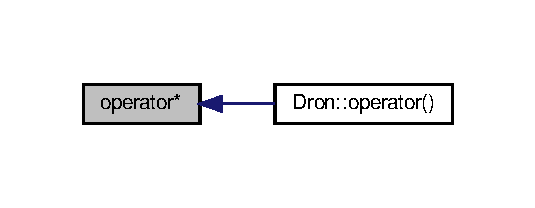
\includegraphics[width=257pt]{_dron_8hh_a8f9219ec11c21cfdb4178a3ccac3ccc8_icgraph}
\end{center}
\end{figure}
\mbox{\Hypertarget{_dron_8hh_a81962db5d5d03dc7f8ff67724c88b57d}\label{_dron_8hh_a81962db5d5d03dc7f8ff67724c88b57d}} 
\index{Dron.\+hh@{Dron.\+hh}!operator+@{operator+}}
\index{operator+@{operator+}!Dron.\+hh@{Dron.\+hh}}
\subsubsection{\texorpdfstring{operator+()}{operator+()}}
{\footnotesize\ttfamily \hyperlink{class_dron}{Dron} operator+ (\begin{DoxyParamCaption}\item[{\hyperlink{class_dron}{Dron}}]{D1,  }\item[{\hyperlink{_wektor3_d_8hh_ac353a272b38b4ad342f7181ad7bdb91a}{Wektor3D}}]{W2 }\end{DoxyParamCaption})}

Here is the caller graph for this function\+:
\nopagebreak
\begin{figure}[H]
\begin{center}
\leavevmode
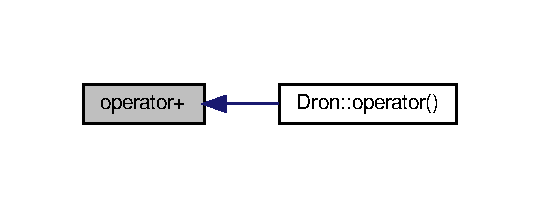
\includegraphics[width=259pt]{_dron_8hh_a81962db5d5d03dc7f8ff67724c88b57d_icgraph}
\end{center}
\end{figure}

\hypertarget{lacze__do__gnuplota_8hh}{}\section{inc/lacze\+\_\+do\+\_\+gnuplota.hh File Reference}
\label{lacze__do__gnuplota_8hh}\index{inc/lacze\+\_\+do\+\_\+gnuplota.\+hh@{inc/lacze\+\_\+do\+\_\+gnuplota.\+hh}}
{\ttfamily \#include $<$string$>$}\newline
{\ttfamily \#include $<$list$>$}\newline
{\ttfamily \#include $<$vector$>$}\newline
Include dependency graph for lacze\+\_\+do\+\_\+gnuplota.\+hh\+:\nopagebreak
\begin{figure}[H]
\begin{center}
\leavevmode
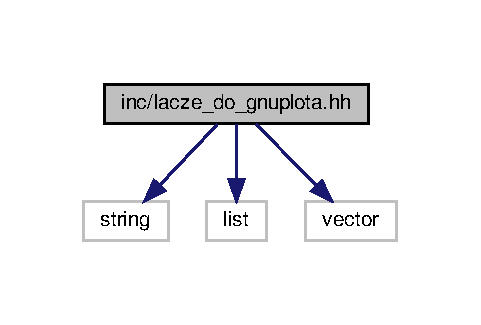
\includegraphics[width=231pt]{lacze__do__gnuplota_8hh__incl}
\end{center}
\end{figure}
This graph shows which files directly or indirectly include this file\+:\nopagebreak
\begin{figure}[H]
\begin{center}
\leavevmode
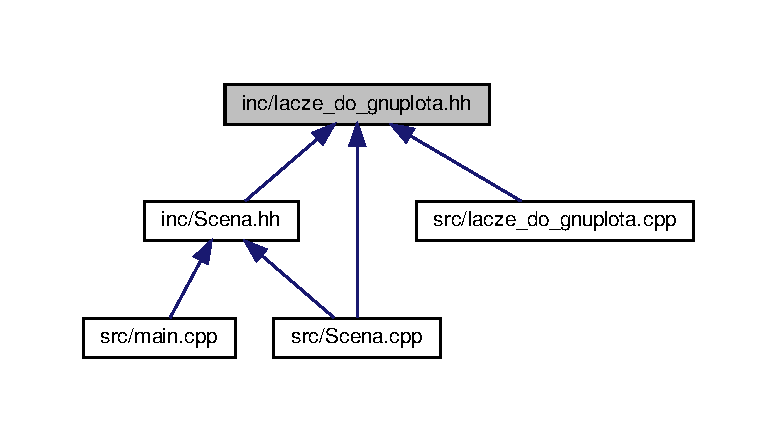
\includegraphics[width=350pt]{lacze__do__gnuplota_8hh__dep__incl}
\end{center}
\end{figure}
\subsection*{Classes}
\begin{DoxyCompactItemize}
\item 
class \hyperlink{class_pz_g_1_1_info_pliku_do_rysowania}{Pz\+G\+::\+Info\+Pliku\+Do\+Rysowania}
\begin{DoxyCompactList}\small\item\em Zestaw informacji dotyczący pliku i sposobu rysowania. \end{DoxyCompactList}\item 
class \hyperlink{class_pz_g_1_1_lacze_do_g_n_u_plota}{Pz\+G\+::\+Lacze\+Do\+G\+N\+U\+Plota}
\begin{DoxyCompactList}\small\item\em Klasa realizuje interfejs do programu G\+N\+U\+Plot. \end{DoxyCompactList}\end{DoxyCompactItemize}
\subsection*{Namespaces}
\begin{DoxyCompactItemize}
\item 
 \hyperlink{namespace_pz_g}{PzG}
\begin{DoxyCompactList}\small\item\em Moduł narzędzi umożliwiających połącznie z G\+N\+U\+Plotem. \end{DoxyCompactList}\end{DoxyCompactItemize}
\subsection*{Enumerations}
\begin{DoxyCompactItemize}
\item 
enum \hyperlink{namespace_pz_g_aeedae1ef10c66d720f9e89de408ca4ca}{Pz\+G\+::\+Tryb\+Rysowania} \{ \hyperlink{namespace_pz_g_aeedae1ef10c66d720f9e89de408ca4caa5eb0cf8b3405e136f092efdb489d60c4}{Pz\+G\+::\+T\+R\+\_\+2D}, 
\hyperlink{namespace_pz_g_aeedae1ef10c66d720f9e89de408ca4caa856e6b0fa6b8a9dc184c60cf27dcc5d2}{Pz\+G\+::\+T\+R\+\_\+3D}
 \}\begin{DoxyCompactList}\small\item\em Określa tryb rysowania realizowanego przez program {\ttfamily gnuplot}. \end{DoxyCompactList}
\item 
enum \hyperlink{namespace_pz_g_a705c92106f39b7d0c34a6739d10ff0b6}{Pz\+G\+::\+Rodzaj\+Rysowania} \{ \hyperlink{namespace_pz_g_a705c92106f39b7d0c34a6739d10ff0b6a927eaa159aa4bd3198f0a330b967746d}{Pz\+G\+::\+R\+R\+\_\+\+Ciagly}, 
\hyperlink{namespace_pz_g_a705c92106f39b7d0c34a6739d10ff0b6aa01097ee8266d6402b752ef6f9a4690c}{Pz\+G\+::\+R\+R\+\_\+\+Punktowy}
 \}\begin{DoxyCompactList}\small\item\em Sposób rysowania linii. \end{DoxyCompactList}
\end{DoxyCompactItemize}


\subsection{Detailed Description}
Plik zawiera definicję klasy realizującej interfejs komunikacyjny do programu gnuplot. 
\hypertarget{_macierz_8hh}{}\section{inc/\+Macierz.hh File Reference}
\label{_macierz_8hh}\index{inc/\+Macierz.\+hh@{inc/\+Macierz.\+hh}}
{\ttfamily \#include $<$iostream$>$}\newline
{\ttfamily \#include $<$tgmath.\+h$>$}\newline
Include dependency graph for Macierz.\+hh\+:\nopagebreak
\begin{figure}[H]
\begin{center}
\leavevmode
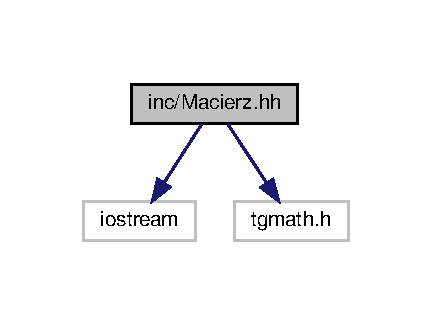
\includegraphics[width=208pt]{_macierz_8hh__incl}
\end{center}
\end{figure}
This graph shows which files directly or indirectly include this file\+:
\nopagebreak
\begin{figure}[H]
\begin{center}
\leavevmode
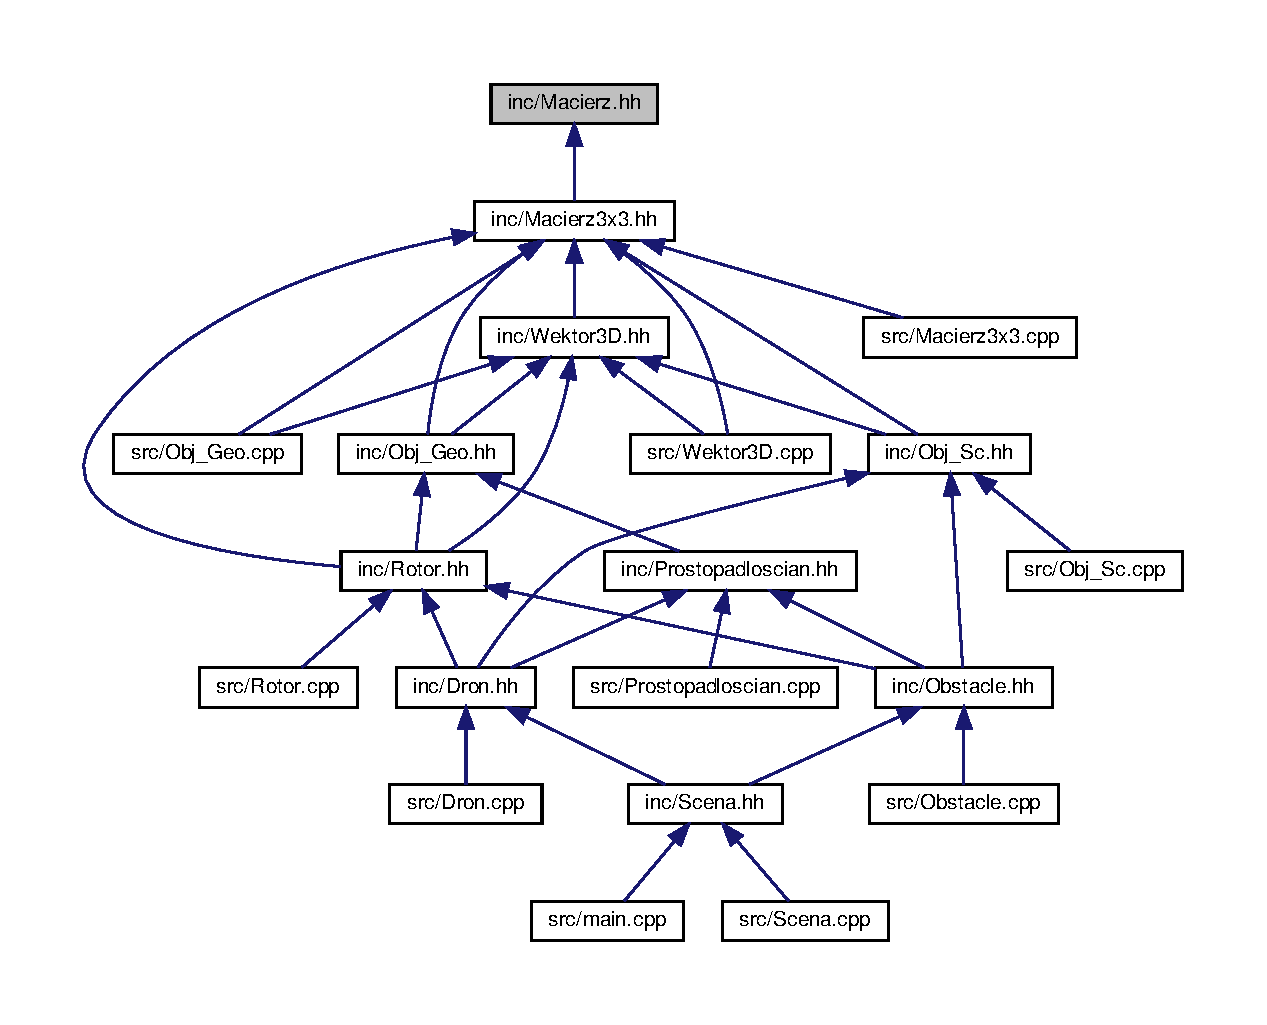
\includegraphics[width=350pt]{_macierz_8hh__dep__incl}
\end{center}
\end{figure}
\subsection*{Classes}
\begin{DoxyCompactItemize}
\item 
class \hyperlink{class_macierz}{Macierz$<$ Wymiar $>$}
\begin{DoxyCompactList}\small\item\em Klasa ta reprezentuje macierz (tablica n-\/wymiarowa, metoda rotacji, przeciążenia operatorów itp). \end{DoxyCompactList}\end{DoxyCompactItemize}

\hypertarget{_macierz3x3_8hh}{}\section{inc/\+Macierz3x3.hh File Reference}
\label{_macierz3x3_8hh}\index{inc/\+Macierz3x3.\+hh@{inc/\+Macierz3x3.\+hh}}
{\ttfamily \#include $<$iostream$>$}\newline
{\ttfamily \#include \char`\"{}Macierz.\+hh\char`\"{}}\newline
Include dependency graph for Macierz3x3.\+hh\+:\nopagebreak
\begin{figure}[H]
\begin{center}
\leavevmode
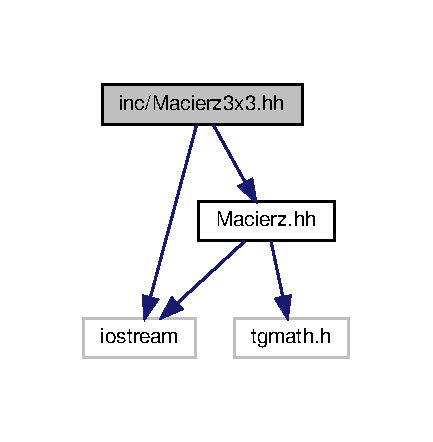
\includegraphics[width=208pt]{_macierz3x3_8hh__incl}
\end{center}
\end{figure}
This graph shows which files directly or indirectly include this file\+:
\nopagebreak
\begin{figure}[H]
\begin{center}
\leavevmode
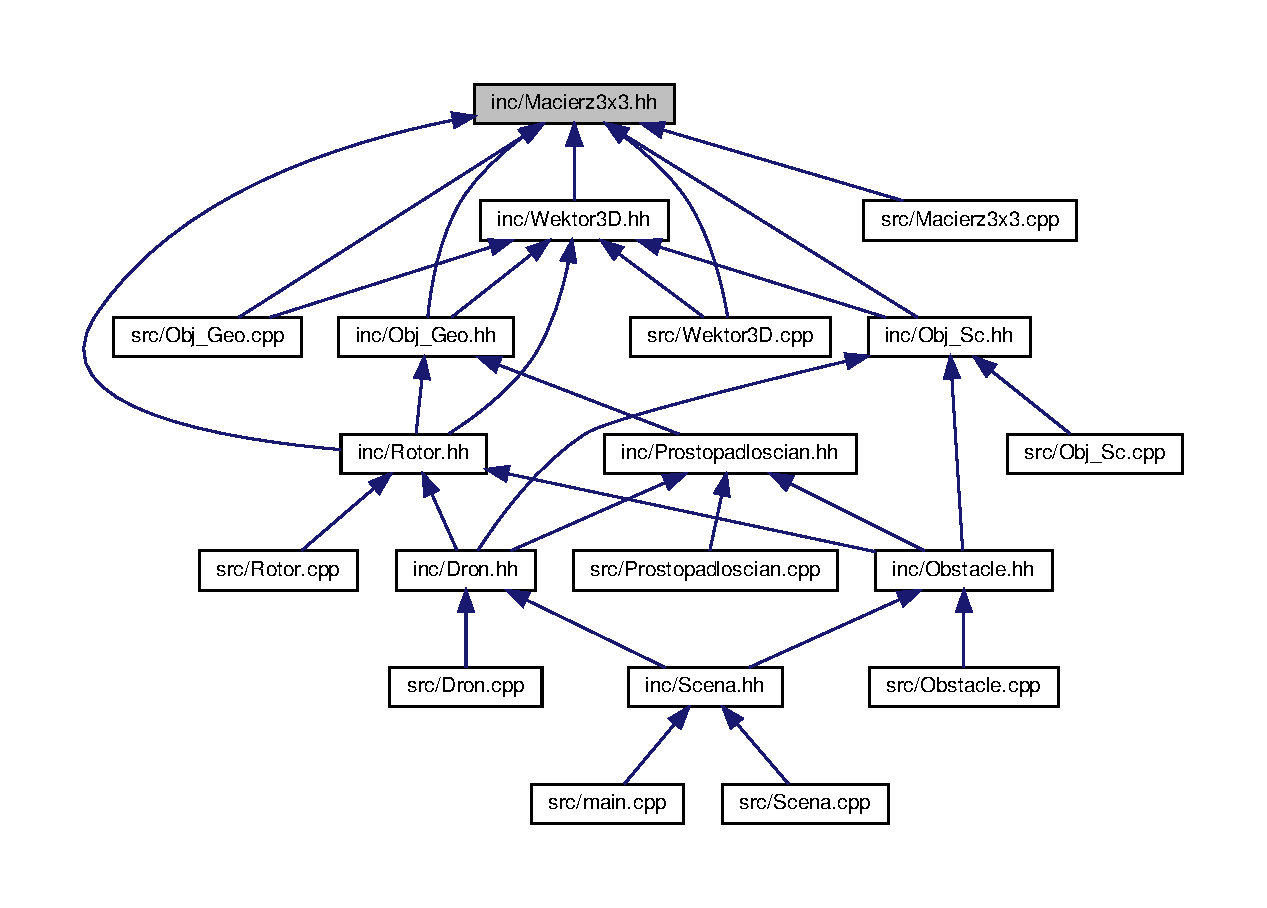
\includegraphics[width=350pt]{_macierz3x3_8hh__dep__incl}
\end{center}
\end{figure}
\subsection*{Typedefs}
\begin{DoxyCompactItemize}
\item 
typedef \hyperlink{class_macierz}{Macierz}$<$ 3 $>$ \hyperlink{_macierz3x3_8hh_ad4fc7b0e263d9a99ba6174f68b52ea87}{Macierz3x3}
\end{DoxyCompactItemize}
\subsection*{Functions}
\begin{DoxyCompactItemize}
\item 
std\+::ostream \& \hyperlink{_macierz3x3_8hh_a7d624426c40b579f848005cc55b24ea6}{operator$<$$<$} (std\+::ostream \&Strm, const \hyperlink{_macierz3x3_8hh_ad4fc7b0e263d9a99ba6174f68b52ea87}{Macierz3x3} \&Mac)
\end{DoxyCompactItemize}


\subsection{Typedef Documentation}
\mbox{\Hypertarget{_macierz3x3_8hh_ad4fc7b0e263d9a99ba6174f68b52ea87}\label{_macierz3x3_8hh_ad4fc7b0e263d9a99ba6174f68b52ea87}} 
\index{Macierz3x3.\+hh@{Macierz3x3.\+hh}!Macierz3x3@{Macierz3x3}}
\index{Macierz3x3@{Macierz3x3}!Macierz3x3.\+hh@{Macierz3x3.\+hh}}
\subsubsection{\texorpdfstring{Macierz3x3}{Macierz3x3}}
{\footnotesize\ttfamily typedef \hyperlink{class_macierz}{Macierz}$<$3$>$ \hyperlink{_macierz3x3_8hh_ad4fc7b0e263d9a99ba6174f68b52ea87}{Macierz3x3}}



Definition at line 8 of file Macierz3x3.\+hh.



\subsection{Function Documentation}
\mbox{\Hypertarget{_macierz3x3_8hh_a7d624426c40b579f848005cc55b24ea6}\label{_macierz3x3_8hh_a7d624426c40b579f848005cc55b24ea6}} 
\index{Macierz3x3.\+hh@{Macierz3x3.\+hh}!operator$<$$<$@{operator$<$$<$}}
\index{operator$<$$<$@{operator$<$$<$}!Macierz3x3.\+hh@{Macierz3x3.\+hh}}
\subsubsection{\texorpdfstring{operator$<$$<$()}{operator<<()}}
{\footnotesize\ttfamily std\+::ostream\& operator$<$$<$ (\begin{DoxyParamCaption}\item[{std\+::ostream \&}]{Strm,  }\item[{const \hyperlink{_macierz3x3_8hh_ad4fc7b0e263d9a99ba6174f68b52ea87}{Macierz3x3} \&}]{Mac }\end{DoxyParamCaption})}



Definition at line 3 of file Macierz3x3.\+cpp.


\hypertarget{_obj___geo_8hh}{}\section{inc/\+Obj\+\_\+\+Geo.hh File Reference}
\label{_obj___geo_8hh}\index{inc/\+Obj\+\_\+\+Geo.\+hh@{inc/\+Obj\+\_\+\+Geo.\+hh}}
{\ttfamily \#include $<$iostream$>$}\newline
{\ttfamily \#include $<$vector$>$}\newline
{\ttfamily \#include \char`\"{}Wektor3\+D.\+hh\char`\"{}}\newline
{\ttfamily \#include \char`\"{}Macierz3x3.\+hh\char`\"{}}\newline
Include dependency graph for Obj\+\_\+\+Geo.\+hh\+:
\nopagebreak
\begin{figure}[H]
\begin{center}
\leavevmode
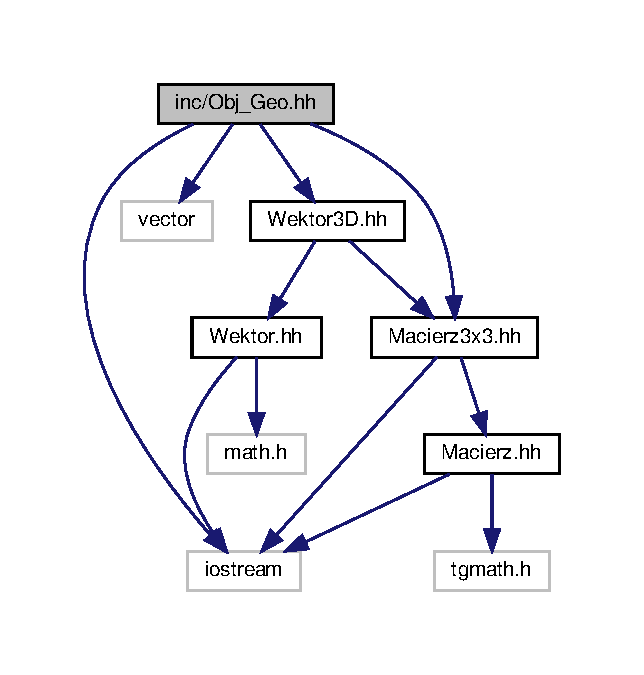
\includegraphics[width=309pt]{_obj___geo_8hh__incl}
\end{center}
\end{figure}
This graph shows which files directly or indirectly include this file\+:
\nopagebreak
\begin{figure}[H]
\begin{center}
\leavevmode
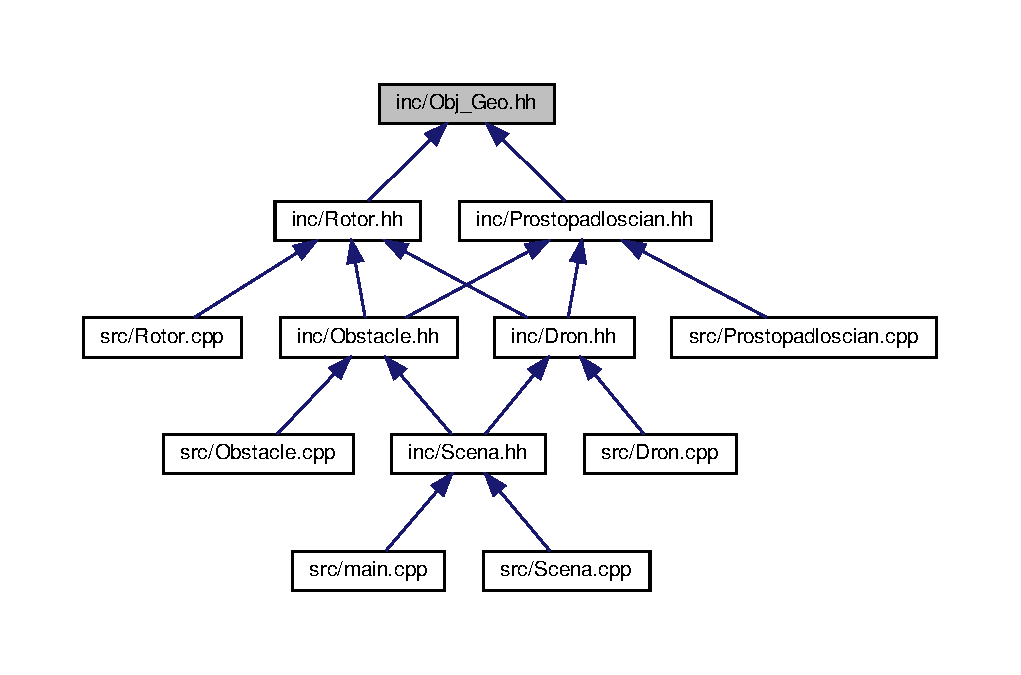
\includegraphics[width=350pt]{_obj___geo_8hh__dep__incl}
\end{center}
\end{figure}
\subsection*{Classes}
\begin{DoxyCompactItemize}
\item 
class \hyperlink{class_obj___geo}{Obj\+\_\+\+Geo}
\end{DoxyCompactItemize}

\hypertarget{_obj___sc_8hh}{}\section{inc/\+Obj\+\_\+\+Sc.hh File Reference}
\label{_obj___sc_8hh}\index{inc/\+Obj\+\_\+\+Sc.\+hh@{inc/\+Obj\+\_\+\+Sc.\+hh}}
{\ttfamily \#include $<$iostream$>$}\newline
{\ttfamily \#include $<$vector$>$}\newline
{\ttfamily \#include \char`\"{}Wektor3\+D.\+hh\char`\"{}}\newline
{\ttfamily \#include \char`\"{}Macierz3x3.\+hh\char`\"{}}\newline
Include dependency graph for Obj\+\_\+\+Sc.\+hh\+:
\nopagebreak
\begin{figure}[H]
\begin{center}
\leavevmode
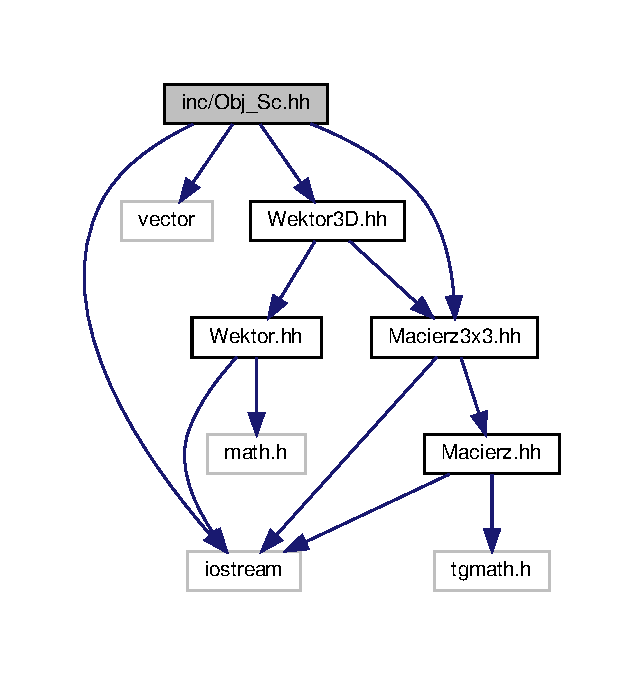
\includegraphics[width=309pt]{_obj___sc_8hh__incl}
\end{center}
\end{figure}
This graph shows which files directly or indirectly include this file\+:
\nopagebreak
\begin{figure}[H]
\begin{center}
\leavevmode
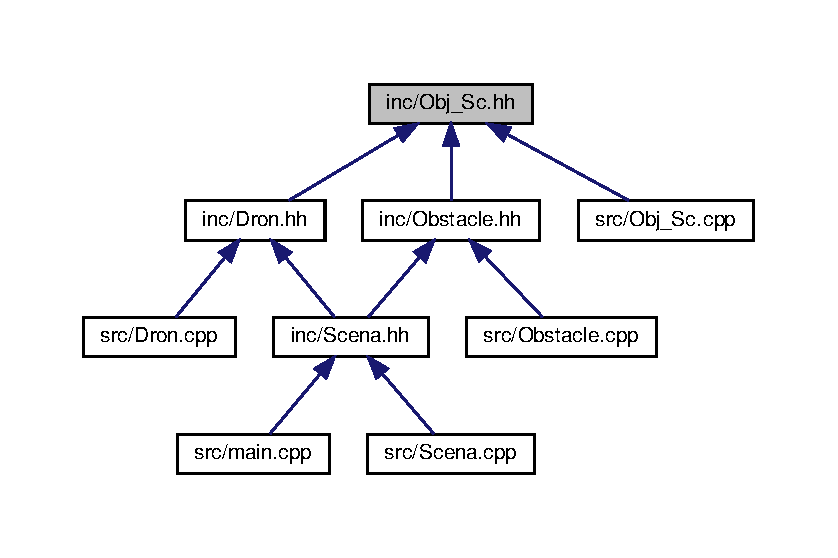
\includegraphics[width=350pt]{_obj___sc_8hh__dep__incl}
\end{center}
\end{figure}
\subsection*{Classes}
\begin{DoxyCompactItemize}
\item 
class \hyperlink{class_obj___sc}{Obj\+\_\+\+Sc}
\begin{DoxyCompactList}\small\item\em Klasa ta jest dziedziczona do drona oraz przeszkody. Jego metodą jest wykrywanie kolizji. \end{DoxyCompactList}\end{DoxyCompactItemize}

\hypertarget{_obstacle_8hh}{}\section{inc/\+Obstacle.hh File Reference}
\label{_obstacle_8hh}\index{inc/\+Obstacle.\+hh@{inc/\+Obstacle.\+hh}}
{\ttfamily \#include $<$iostream$>$}\newline
{\ttfamily \#include \char`\"{}Prostopadloscian.\+hh\char`\"{}}\newline
{\ttfamily \#include \char`\"{}Rotor.\+hh\char`\"{}}\newline
{\ttfamily \#include \char`\"{}Obj\+\_\+\+Sc.\+hh\char`\"{}}\newline
Include dependency graph for Obstacle.\+hh\+:
\nopagebreak
\begin{figure}[H]
\begin{center}
\leavevmode
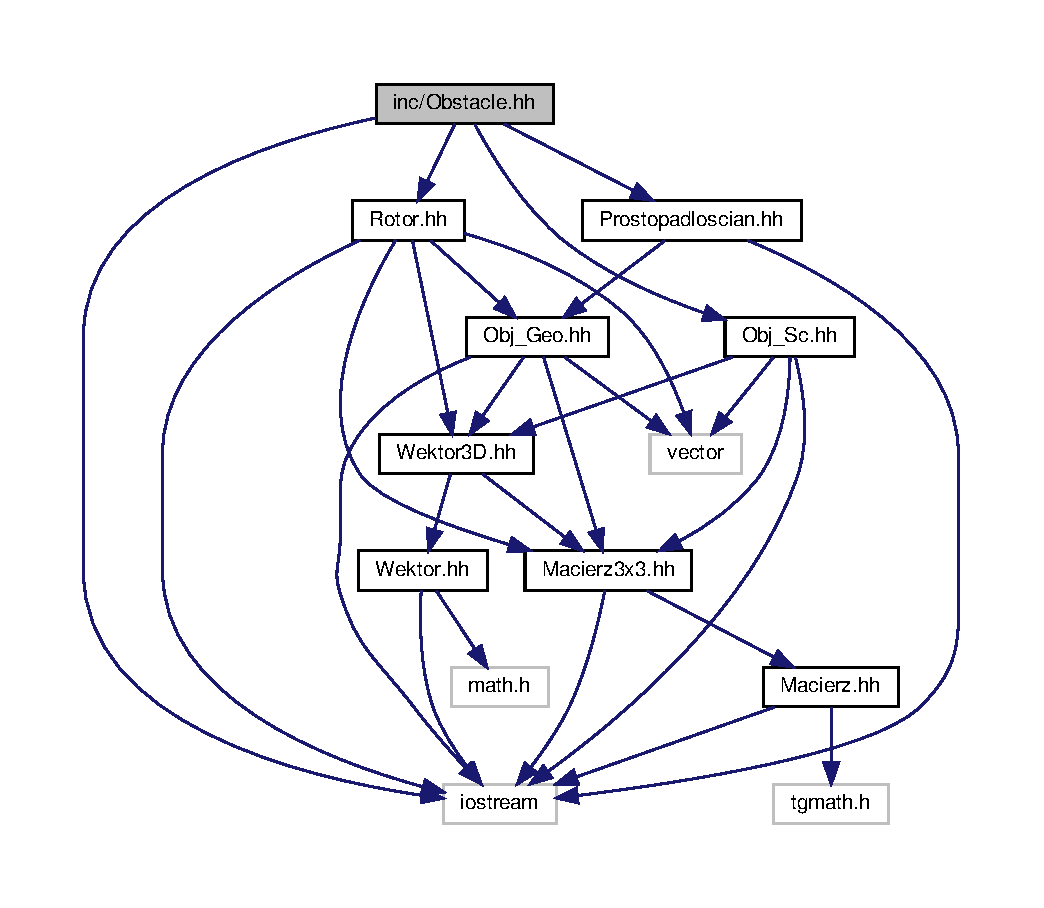
\includegraphics[width=350pt]{_obstacle_8hh__incl}
\end{center}
\end{figure}
This graph shows which files directly or indirectly include this file\+:
\nopagebreak
\begin{figure}[H]
\begin{center}
\leavevmode
\includegraphics[width=310pt]{_obstacle_8hh__dep__incl}
\end{center}
\end{figure}
\subsection*{Classes}
\begin{DoxyCompactItemize}
\item 
class \hyperlink{class_obstacle}{Obstacle}
\begin{DoxyCompactList}\small\item\em Klasa określa przeszkode. Jest fragmentem objektu sceny. \end{DoxyCompactList}\end{DoxyCompactItemize}

\hypertarget{_prostopadloscian_8hh}{}\section{inc/\+Prostopadloscian.hh File Reference}
\label{_prostopadloscian_8hh}\index{inc/\+Prostopadloscian.\+hh@{inc/\+Prostopadloscian.\+hh}}
{\ttfamily \#include $<$iostream$>$}\newline
{\ttfamily \#include \char`\"{}Obj\+\_\+\+Geo.\+hh\char`\"{}}\newline
Include dependency graph for Prostopadloscian.\+hh\+:
\nopagebreak
\begin{figure}[H]
\begin{center}
\leavevmode
\includegraphics[width=350pt]{_prostopadloscian_8hh__incl}
\end{center}
\end{figure}
This graph shows which files directly or indirectly include this file\+:
\nopagebreak
\begin{figure}[H]
\begin{center}
\leavevmode
\includegraphics[width=350pt]{_prostopadloscian_8hh__dep__incl}
\end{center}
\end{figure}
\subsection*{Classes}
\begin{DoxyCompactItemize}
\item 
class \hyperlink{class_prostopadloscian}{Prostopadloscian}
\begin{DoxyCompactList}\small\item\em Klasa ta reprezentuje prostopadłościan oraz to co go określa (współrzędne, metody obrotu, translacji itp). \end{DoxyCompactList}\end{DoxyCompactItemize}
\subsection*{Functions}
\begin{DoxyCompactItemize}
\item 
std\+::ostream \& \hyperlink{_prostopadloscian_8hh_a0a77f9bb1cc3f07e11031b947e6e7322}{operator$<$$<$} (std\+::ostream \&Strm, const \hyperlink{class_prostopadloscian}{Prostopadloscian} \&Pr)
\item 
\hyperlink{class_prostopadloscian}{Prostopadloscian} \hyperlink{_prostopadloscian_8hh_a0c34886e02f7ad596e7ae26ef4bdc44f}{operator$\ast$} (\hyperlink{_macierz3x3_8hh_ad4fc7b0e263d9a99ba6174f68b52ea87}{Macierz3x3} M, \hyperlink{class_prostopadloscian}{Prostopadloscian} P)
\item 
\hyperlink{class_prostopadloscian}{Prostopadloscian} \hyperlink{_prostopadloscian_8hh_aed7fb32f55c347f1ffbbdb209d41fa04}{operator+} (\hyperlink{class_prostopadloscian}{Prostopadloscian} P1, \hyperlink{_wektor3_d_8hh_ac353a272b38b4ad342f7181ad7bdb91a}{Wektor3D} W2)
\item 
\hyperlink{class_prostopadloscian}{Prostopadloscian} \hyperlink{_prostopadloscian_8hh_ae86d86b37f5a8a4fb819b121ef0473d5}{operator+} (\hyperlink{class_prostopadloscian}{Prostopadloscian} P1, \hyperlink{class_prostopadloscian}{Prostopadloscian} P2)
\item 
std\+::istream \& \hyperlink{_prostopadloscian_8hh_a002ba87e7198bb0f1a42575278b379d8}{operator$>$$>$} (std\+::istream \&Strm, \hyperlink{class_prostopadloscian}{Prostopadloscian} \&Pr)
\end{DoxyCompactItemize}


\subsection{Function Documentation}
\mbox{\Hypertarget{_prostopadloscian_8hh_a0c34886e02f7ad596e7ae26ef4bdc44f}\label{_prostopadloscian_8hh_a0c34886e02f7ad596e7ae26ef4bdc44f}} 
\index{Prostopadloscian.\+hh@{Prostopadloscian.\+hh}!operator$\ast$@{operator$\ast$}}
\index{operator$\ast$@{operator$\ast$}!Prostopadloscian.\+hh@{Prostopadloscian.\+hh}}
\subsubsection{\texorpdfstring{operator$\ast$()}{operator*()}}
{\footnotesize\ttfamily \hyperlink{class_prostopadloscian}{Prostopadloscian} operator$\ast$ (\begin{DoxyParamCaption}\item[{\hyperlink{_macierz3x3_8hh_ad4fc7b0e263d9a99ba6174f68b52ea87}{Macierz3x3}}]{M,  }\item[{\hyperlink{class_prostopadloscian}{Prostopadloscian}}]{P }\end{DoxyParamCaption})}



Definition at line 57 of file Prostopadloscian.\+cpp.

Here is the caller graph for this function\+:\nopagebreak
\begin{figure}[H]
\begin{center}
\leavevmode
\includegraphics[width=311pt]{_prostopadloscian_8hh_a0c34886e02f7ad596e7ae26ef4bdc44f_icgraph}
\end{center}
\end{figure}
\mbox{\Hypertarget{_prostopadloscian_8hh_aed7fb32f55c347f1ffbbdb209d41fa04}\label{_prostopadloscian_8hh_aed7fb32f55c347f1ffbbdb209d41fa04}} 
\index{Prostopadloscian.\+hh@{Prostopadloscian.\+hh}!operator+@{operator+}}
\index{operator+@{operator+}!Prostopadloscian.\+hh@{Prostopadloscian.\+hh}}
\subsubsection{\texorpdfstring{operator+()}{operator+()}\hspace{0.1cm}{\footnotesize\ttfamily [1/2]}}
{\footnotesize\ttfamily \hyperlink{class_prostopadloscian}{Prostopadloscian} operator+ (\begin{DoxyParamCaption}\item[{\hyperlink{class_prostopadloscian}{Prostopadloscian}}]{P1,  }\item[{\hyperlink{_wektor3_d_8hh_ac353a272b38b4ad342f7181ad7bdb91a}{Wektor3D}}]{W2 }\end{DoxyParamCaption})}



Definition at line 66 of file Prostopadloscian.\+cpp.

Here is the caller graph for this function\+:\nopagebreak
\begin{figure}[H]
\begin{center}
\leavevmode
\includegraphics[width=313pt]{_prostopadloscian_8hh_aed7fb32f55c347f1ffbbdb209d41fa04_icgraph}
\end{center}
\end{figure}
\mbox{\Hypertarget{_prostopadloscian_8hh_ae86d86b37f5a8a4fb819b121ef0473d5}\label{_prostopadloscian_8hh_ae86d86b37f5a8a4fb819b121ef0473d5}} 
\index{Prostopadloscian.\+hh@{Prostopadloscian.\+hh}!operator+@{operator+}}
\index{operator+@{operator+}!Prostopadloscian.\+hh@{Prostopadloscian.\+hh}}
\subsubsection{\texorpdfstring{operator+()}{operator+()}\hspace{0.1cm}{\footnotesize\ttfamily [2/2]}}
{\footnotesize\ttfamily \hyperlink{class_prostopadloscian}{Prostopadloscian} operator+ (\begin{DoxyParamCaption}\item[{\hyperlink{class_prostopadloscian}{Prostopadloscian}}]{P1,  }\item[{\hyperlink{class_prostopadloscian}{Prostopadloscian}}]{P2 }\end{DoxyParamCaption})}



Definition at line 76 of file Prostopadloscian.\+cpp.

\mbox{\Hypertarget{_prostopadloscian_8hh_a0a77f9bb1cc3f07e11031b947e6e7322}\label{_prostopadloscian_8hh_a0a77f9bb1cc3f07e11031b947e6e7322}} 
\index{Prostopadloscian.\+hh@{Prostopadloscian.\+hh}!operator$<$$<$@{operator$<$$<$}}
\index{operator$<$$<$@{operator$<$$<$}!Prostopadloscian.\+hh@{Prostopadloscian.\+hh}}
\subsubsection{\texorpdfstring{operator$<$$<$()}{operator<<()}}
{\footnotesize\ttfamily std\+::ostream\& operator$<$$<$ (\begin{DoxyParamCaption}\item[{std\+::ostream \&}]{Strm,  }\item[{const \hyperlink{class_prostopadloscian}{Prostopadloscian} \&}]{Pr }\end{DoxyParamCaption})}



Definition at line 43 of file Prostopadloscian.\+cpp.

Here is the caller graph for this function\+:\nopagebreak
\begin{figure}[H]
\begin{center}
\leavevmode
\includegraphics[width=319pt]{_prostopadloscian_8hh_a0a77f9bb1cc3f07e11031b947e6e7322_icgraph}
\end{center}
\end{figure}
\mbox{\Hypertarget{_prostopadloscian_8hh_a002ba87e7198bb0f1a42575278b379d8}\label{_prostopadloscian_8hh_a002ba87e7198bb0f1a42575278b379d8}} 
\index{Prostopadloscian.\+hh@{Prostopadloscian.\+hh}!operator$>$$>$@{operator$>$$>$}}
\index{operator$>$$>$@{operator$>$$>$}!Prostopadloscian.\+hh@{Prostopadloscian.\+hh}}
\subsubsection{\texorpdfstring{operator$>$$>$()}{operator>>()}}
{\footnotesize\ttfamily std\+::istream\& operator$>$$>$ (\begin{DoxyParamCaption}\item[{std\+::istream \&}]{Strm,  }\item[{\hyperlink{class_prostopadloscian}{Prostopadloscian} \&}]{Pr }\end{DoxyParamCaption})}



Definition at line 84 of file Prostopadloscian.\+cpp.

Here is the call graph for this function\+:
\nopagebreak
\begin{figure}[H]
\begin{center}
\leavevmode
\includegraphics[width=323pt]{_prostopadloscian_8hh_a002ba87e7198bb0f1a42575278b379d8_cgraph}
\end{center}
\end{figure}
Here is the caller graph for this function\+:
\nopagebreak
\begin{figure}[H]
\begin{center}
\leavevmode
\includegraphics[width=319pt]{_prostopadloscian_8hh_a002ba87e7198bb0f1a42575278b379d8_icgraph}
\end{center}
\end{figure}

\hypertarget{_rotor_8hh}{}\section{inc/\+Rotor.hh File Reference}
\label{_rotor_8hh}\index{inc/\+Rotor.\+hh@{inc/\+Rotor.\+hh}}
{\ttfamily \#include $<$iostream$>$}\newline
{\ttfamily \#include $<$vector$>$}\newline
{\ttfamily \#include \char`\"{}Wektor3\+D.\+hh\char`\"{}}\newline
{\ttfamily \#include \char`\"{}Macierz3x3.\+hh\char`\"{}}\newline
{\ttfamily \#include \char`\"{}Obj\+\_\+\+Geo.\+hh\char`\"{}}\newline
Include dependency graph for Rotor.\+hh\+:
\nopagebreak
\begin{figure}[H]
\begin{center}
\leavevmode
\includegraphics[width=350pt]{_rotor_8hh__incl}
\end{center}
\end{figure}
This graph shows which files directly or indirectly include this file\+:
\nopagebreak
\begin{figure}[H]
\begin{center}
\leavevmode
\includegraphics[width=350pt]{_rotor_8hh__dep__incl}
\end{center}
\end{figure}
\subsection*{Classes}
\begin{DoxyCompactItemize}
\item 
class \hyperlink{class_rotor}{Rotor}
\begin{DoxyCompactList}\small\item\em Klasa określa współrzędne rotorów oraz jak się obracają \end{DoxyCompactList}\end{DoxyCompactItemize}
\subsection*{Functions}
\begin{DoxyCompactItemize}
\item 
std\+::ostream \& \hyperlink{_rotor_8hh_a6e6ce3bcc6ad0cb16d457ac8d73b3a7e}{operator$<$$<$} (std\+::ostream \&Strm, const \hyperlink{class_rotor}{Rotor} \&Pr)
\item 
\hyperlink{class_rotor}{Rotor} \hyperlink{_rotor_8hh_a66cbe78735e95530c8eb1361b6fe40eb}{operator$\ast$} (\hyperlink{_macierz3x3_8hh_ad4fc7b0e263d9a99ba6174f68b52ea87}{Macierz3x3} M, \hyperlink{class_rotor}{Rotor} P)
\item 
\hyperlink{class_rotor}{Rotor} \hyperlink{_rotor_8hh_a8e627d5e28005e4dc3a7ab7ae6e21f9b}{operator+} (\hyperlink{class_rotor}{Rotor} P1, \hyperlink{_wektor3_d_8hh_ac353a272b38b4ad342f7181ad7bdb91a}{Wektor3D} W2)
\item 
\hyperlink{class_rotor}{Rotor} \hyperlink{_rotor_8hh_aec4621815bb6b2569f3c34689e7533a8}{operator+} (\hyperlink{class_rotor}{Rotor} P1, \hyperlink{class_rotor}{Rotor} P2)
\item 
std\+::istream \& \hyperlink{_rotor_8hh_a2e505b0dd49c9d2cb7fb02a9ea8ad231}{operator$>$$>$} (std\+::istream \&Strm, \hyperlink{class_rotor}{Rotor} \&Pr)
\end{DoxyCompactItemize}


\subsection{Function Documentation}
\mbox{\Hypertarget{_rotor_8hh_a66cbe78735e95530c8eb1361b6fe40eb}\label{_rotor_8hh_a66cbe78735e95530c8eb1361b6fe40eb}} 
\index{Rotor.\+hh@{Rotor.\+hh}!operator$\ast$@{operator$\ast$}}
\index{operator$\ast$@{operator$\ast$}!Rotor.\+hh@{Rotor.\+hh}}
\subsubsection{\texorpdfstring{operator$\ast$()}{operator*()}}
{\footnotesize\ttfamily \hyperlink{class_rotor}{Rotor} operator$\ast$ (\begin{DoxyParamCaption}\item[{\hyperlink{_macierz3x3_8hh_ad4fc7b0e263d9a99ba6174f68b52ea87}{Macierz3x3}}]{M,  }\item[{\hyperlink{class_rotor}{Rotor}}]{P }\end{DoxyParamCaption})}



Definition at line 38 of file Rotor.\+cpp.

Here is the caller graph for this function\+:
\nopagebreak
\begin{figure}[H]
\begin{center}
\leavevmode
\includegraphics[width=260pt]{_rotor_8hh_a66cbe78735e95530c8eb1361b6fe40eb_icgraph}
\end{center}
\end{figure}
\mbox{\Hypertarget{_rotor_8hh_a8e627d5e28005e4dc3a7ab7ae6e21f9b}\label{_rotor_8hh_a8e627d5e28005e4dc3a7ab7ae6e21f9b}} 
\index{Rotor.\+hh@{Rotor.\+hh}!operator+@{operator+}}
\index{operator+@{operator+}!Rotor.\+hh@{Rotor.\+hh}}
\subsubsection{\texorpdfstring{operator+()}{operator+()}\hspace{0.1cm}{\footnotesize\ttfamily [1/2]}}
{\footnotesize\ttfamily \hyperlink{class_rotor}{Rotor} operator+ (\begin{DoxyParamCaption}\item[{\hyperlink{class_rotor}{Rotor}}]{P1,  }\item[{\hyperlink{_wektor3_d_8hh_ac353a272b38b4ad342f7181ad7bdb91a}{Wektor3D}}]{W2 }\end{DoxyParamCaption})}



Definition at line 47 of file Rotor.\+cpp.

Here is the caller graph for this function\+:
\nopagebreak
\begin{figure}[H]
\begin{center}
\leavevmode
\includegraphics[width=262pt]{_rotor_8hh_a8e627d5e28005e4dc3a7ab7ae6e21f9b_icgraph}
\end{center}
\end{figure}
\mbox{\Hypertarget{_rotor_8hh_aec4621815bb6b2569f3c34689e7533a8}\label{_rotor_8hh_aec4621815bb6b2569f3c34689e7533a8}} 
\index{Rotor.\+hh@{Rotor.\+hh}!operator+@{operator+}}
\index{operator+@{operator+}!Rotor.\+hh@{Rotor.\+hh}}
\subsubsection{\texorpdfstring{operator+()}{operator+()}\hspace{0.1cm}{\footnotesize\ttfamily [2/2]}}
{\footnotesize\ttfamily \hyperlink{class_rotor}{Rotor} operator+ (\begin{DoxyParamCaption}\item[{\hyperlink{class_rotor}{Rotor}}]{P1,  }\item[{\hyperlink{class_rotor}{Rotor}}]{P2 }\end{DoxyParamCaption})}



Definition at line 57 of file Rotor.\+cpp.

\mbox{\Hypertarget{_rotor_8hh_a6e6ce3bcc6ad0cb16d457ac8d73b3a7e}\label{_rotor_8hh_a6e6ce3bcc6ad0cb16d457ac8d73b3a7e}} 
\index{Rotor.\+hh@{Rotor.\+hh}!operator$<$$<$@{operator$<$$<$}}
\index{operator$<$$<$@{operator$<$$<$}!Rotor.\+hh@{Rotor.\+hh}}
\subsubsection{\texorpdfstring{operator$<$$<$()}{operator<<()}}
{\footnotesize\ttfamily std\+::ostream\& operator$<$$<$ (\begin{DoxyParamCaption}\item[{std\+::ostream \&}]{Strm,  }\item[{const \hyperlink{class_rotor}{Rotor} \&}]{Pr }\end{DoxyParamCaption})}



Definition at line 26 of file Rotor.\+cpp.

Here is the caller graph for this function\+:
\nopagebreak
\begin{figure}[H]
\begin{center}
\leavevmode
\includegraphics[width=268pt]{_rotor_8hh_a6e6ce3bcc6ad0cb16d457ac8d73b3a7e_icgraph}
\end{center}
\end{figure}
\mbox{\Hypertarget{_rotor_8hh_a2e505b0dd49c9d2cb7fb02a9ea8ad231}\label{_rotor_8hh_a2e505b0dd49c9d2cb7fb02a9ea8ad231}} 
\index{Rotor.\+hh@{Rotor.\+hh}!operator$>$$>$@{operator$>$$>$}}
\index{operator$>$$>$@{operator$>$$>$}!Rotor.\+hh@{Rotor.\+hh}}
\subsubsection{\texorpdfstring{operator$>$$>$()}{operator>>()}}
{\footnotesize\ttfamily std\+::istream\& operator$>$$>$ (\begin{DoxyParamCaption}\item[{std\+::istream \&}]{Strm,  }\item[{\hyperlink{class_rotor}{Rotor} \&}]{Pr }\end{DoxyParamCaption})}



Definition at line 65 of file Rotor.\+cpp.

Here is the call graph for this function\+:
\nopagebreak
\begin{figure}[H]
\begin{center}
\leavevmode
\includegraphics[width=272pt]{_rotor_8hh_a2e505b0dd49c9d2cb7fb02a9ea8ad231_cgraph}
\end{center}
\end{figure}
Here is the caller graph for this function\+:
\nopagebreak
\begin{figure}[H]
\begin{center}
\leavevmode
\includegraphics[width=268pt]{_rotor_8hh_a2e505b0dd49c9d2cb7fb02a9ea8ad231_icgraph}
\end{center}
\end{figure}

\hypertarget{_scena_8hh}{}\section{inc/\+Scena.hh File Reference}
\label{_scena_8hh}\index{inc/\+Scena.\+hh@{inc/\+Scena.\+hh}}
{\ttfamily \#include $<$iostream$>$}\newline
{\ttfamily \#include \char`\"{}lacze\+\_\+do\+\_\+gnuplota.\+hh\char`\"{}}\newline
{\ttfamily \#include \char`\"{}Dron.\+hh\char`\"{}}\newline
{\ttfamily \#include \char`\"{}Obstacle.\+hh\char`\"{}}\newline
{\ttfamily \#include $<$memory$>$}\newline
Include dependency graph for Scena.\+hh\+:
\nopagebreak
\begin{figure}[H]
\begin{center}
\leavevmode
\includegraphics[width=350pt]{_scena_8hh__incl}
\end{center}
\end{figure}
This graph shows which files directly or indirectly include this file\+:
\nopagebreak
\begin{figure}[H]
\begin{center}
\leavevmode
\includegraphics[width=252pt]{_scena_8hh__dep__incl}
\end{center}
\end{figure}
\subsection*{Classes}
\begin{DoxyCompactItemize}
\item 
class \hyperlink{class_scena}{Scena}
\begin{DoxyCompactList}\small\item\em Klasa ta reprezentuje scene. Jego polami to lista objektów scen oraz dronów. \end{DoxyCompactList}\end{DoxyCompactItemize}

\hypertarget{_wektor_8hh}{}\section{inc/\+Wektor.hh File Reference}
\label{_wektor_8hh}\index{inc/\+Wektor.\+hh@{inc/\+Wektor.\+hh}}
{\ttfamily \#include $<$iostream$>$}\newline
{\ttfamily \#include $<$math.\+h$>$}\newline
Include dependency graph for Wektor.\+hh\+:\nopagebreak
\begin{figure}[H]
\begin{center}
\leavevmode
\includegraphics[width=200pt]{_wektor_8hh__incl}
\end{center}
\end{figure}
This graph shows which files directly or indirectly include this file\+:
\nopagebreak
\begin{figure}[H]
\begin{center}
\leavevmode
\includegraphics[width=350pt]{_wektor_8hh__dep__incl}
\end{center}
\end{figure}
\subsection*{Classes}
\begin{DoxyCompactItemize}
\item 
class \hyperlink{class_wektor}{Wektor$<$ Wymiar $>$}
\begin{DoxyCompactList}\small\item\em Klasa ta reprezentuje wektor (tablica n-\/wymiarowa, przeciążenia operatorów itp). \end{DoxyCompactList}\end{DoxyCompactItemize}

\hypertarget{_wektor3_d_8hh}{}\section{inc/\+Wektor3D.hh File Reference}
\label{_wektor3_d_8hh}\index{inc/\+Wektor3\+D.\+hh@{inc/\+Wektor3\+D.\+hh}}
{\ttfamily \#include \char`\"{}Wektor.\+hh\char`\"{}}\newline
{\ttfamily \#include \char`\"{}Macierz3x3.\+hh\char`\"{}}\newline
Include dependency graph for Wektor3\+D.\+hh\+:\nopagebreak
\begin{figure}[H]
\begin{center}
\leavevmode
\includegraphics[width=277pt]{_wektor3_d_8hh__incl}
\end{center}
\end{figure}
This graph shows which files directly or indirectly include this file\+:
\nopagebreak
\begin{figure}[H]
\begin{center}
\leavevmode
\includegraphics[width=350pt]{_wektor3_d_8hh__dep__incl}
\end{center}
\end{figure}
\subsection*{Typedefs}
\begin{DoxyCompactItemize}
\item 
typedef \hyperlink{class_wektor}{Wektor}$<$ 3 $>$ \hyperlink{_wektor3_d_8hh_ac353a272b38b4ad342f7181ad7bdb91a}{Wektor3D}
\end{DoxyCompactItemize}
\subsection*{Functions}
\begin{DoxyCompactItemize}
\item 
\hyperlink{_wektor3_d_8hh_ac353a272b38b4ad342f7181ad7bdb91a}{Wektor3D} \hyperlink{_wektor3_d_8hh_a5441b11ac93c93e38a11a796d1855fe3}{operator$\ast$} (\hyperlink{_macierz3x3_8hh_ad4fc7b0e263d9a99ba6174f68b52ea87}{Macierz3x3} M, \hyperlink{_wektor3_d_8hh_ac353a272b38b4ad342f7181ad7bdb91a}{Wektor3D} V)
\item 
\hyperlink{_wektor3_d_8hh_ac353a272b38b4ad342f7181ad7bdb91a}{Wektor3D} \hyperlink{_wektor3_d_8hh_a11c35b770aab1dd49984861ed1d351d4}{operator$\ast$} (\hyperlink{_wektor3_d_8hh_ac353a272b38b4ad342f7181ad7bdb91a}{Wektor3D} V1, \hyperlink{_wektor3_d_8hh_ac353a272b38b4ad342f7181ad7bdb91a}{Wektor3D} V2)
\item 
double \hyperlink{_wektor3_d_8hh_ac3cbaa36ffda58b46bbaa95b99fde093}{operator\&} (\hyperlink{_wektor3_d_8hh_ac353a272b38b4ad342f7181ad7bdb91a}{Wektor3D} V1, \hyperlink{_wektor3_d_8hh_ac353a272b38b4ad342f7181ad7bdb91a}{Wektor3D} V2)
\item 
\hyperlink{_wektor3_d_8hh_ac353a272b38b4ad342f7181ad7bdb91a}{Wektor3D} \hyperlink{_wektor3_d_8hh_a13099aac77d6145b462434c84f6b8509}{operator$\ast$} (double value, \hyperlink{_wektor3_d_8hh_ac353a272b38b4ad342f7181ad7bdb91a}{Wektor3D} V)
\item 
\hyperlink{_wektor3_d_8hh_ac353a272b38b4ad342f7181ad7bdb91a}{Wektor3D} \hyperlink{_wektor3_d_8hh_a1de808fbd72c8b788a0a88ac119b8a81}{operator+} (\hyperlink{_wektor3_d_8hh_ac353a272b38b4ad342f7181ad7bdb91a}{Wektor3D} W1, \hyperlink{_wektor3_d_8hh_ac353a272b38b4ad342f7181ad7bdb91a}{Wektor3D} W2)
\item 
\hyperlink{_wektor3_d_8hh_ac353a272b38b4ad342f7181ad7bdb91a}{Wektor3D} \hyperlink{_wektor3_d_8hh_a71e2010b0b6abfb4e8a6507eb5c9ebe5}{operator-\/} (\hyperlink{_wektor3_d_8hh_ac353a272b38b4ad342f7181ad7bdb91a}{Wektor3D} W1, \hyperlink{_wektor3_d_8hh_ac353a272b38b4ad342f7181ad7bdb91a}{Wektor3D} W2)
\item 
std\+::istream \& \hyperlink{_wektor3_d_8hh_a1075392800748e0563d8b2c02640a458}{operator$>$$>$} (std\+::istream \&Strm, \hyperlink{_wektor3_d_8hh_ac353a272b38b4ad342f7181ad7bdb91a}{Wektor3D} \&Wek)
\item 
std\+::ostream \& \hyperlink{_wektor3_d_8hh_a55d3a49ea2a060a1d4712feb3811e68e}{operator$<$$<$} (std\+::ostream \&Strm, const \hyperlink{_wektor3_d_8hh_ac353a272b38b4ad342f7181ad7bdb91a}{Wektor3D} \&Wek)
\end{DoxyCompactItemize}


\subsection{Typedef Documentation}
\mbox{\Hypertarget{_wektor3_d_8hh_ac353a272b38b4ad342f7181ad7bdb91a}\label{_wektor3_d_8hh_ac353a272b38b4ad342f7181ad7bdb91a}} 
\index{Wektor3\+D.\+hh@{Wektor3\+D.\+hh}!Wektor3D@{Wektor3D}}
\index{Wektor3D@{Wektor3D}!Wektor3\+D.\+hh@{Wektor3\+D.\+hh}}
\subsubsection{\texorpdfstring{Wektor3D}{Wektor3D}}
{\footnotesize\ttfamily typedef \hyperlink{class_wektor}{Wektor}$<$3$>$ \hyperlink{_wektor3_d_8hh_ac353a272b38b4ad342f7181ad7bdb91a}{Wektor3D}}



Definition at line 8 of file Wektor3\+D.\+hh.



\subsection{Function Documentation}
\mbox{\Hypertarget{_wektor3_d_8hh_ac3cbaa36ffda58b46bbaa95b99fde093}\label{_wektor3_d_8hh_ac3cbaa36ffda58b46bbaa95b99fde093}} 
\index{Wektor3\+D.\+hh@{Wektor3\+D.\+hh}!operator\&@{operator\&}}
\index{operator\&@{operator\&}!Wektor3\+D.\+hh@{Wektor3\+D.\+hh}}
\subsubsection{\texorpdfstring{operator\&()}{operator\&()}}
{\footnotesize\ttfamily double operator \& (\begin{DoxyParamCaption}\item[{\hyperlink{_wektor3_d_8hh_ac353a272b38b4ad342f7181ad7bdb91a}{Wektor3D}}]{V1,  }\item[{\hyperlink{_wektor3_d_8hh_ac353a272b38b4ad342f7181ad7bdb91a}{Wektor3D}}]{V2 }\end{DoxyParamCaption})}



Definition at line 25 of file Wektor3\+D.\+cpp.

\mbox{\Hypertarget{_wektor3_d_8hh_a5441b11ac93c93e38a11a796d1855fe3}\label{_wektor3_d_8hh_a5441b11ac93c93e38a11a796d1855fe3}} 
\index{Wektor3\+D.\+hh@{Wektor3\+D.\+hh}!operator$\ast$@{operator$\ast$}}
\index{operator$\ast$@{operator$\ast$}!Wektor3\+D.\+hh@{Wektor3\+D.\+hh}}
\subsubsection{\texorpdfstring{operator$\ast$()}{operator*()}\hspace{0.1cm}{\footnotesize\ttfamily [1/3]}}
{\footnotesize\ttfamily \hyperlink{_wektor3_d_8hh_ac353a272b38b4ad342f7181ad7bdb91a}{Wektor3D} operator$\ast$ (\begin{DoxyParamCaption}\item[{\hyperlink{_macierz3x3_8hh_ad4fc7b0e263d9a99ba6174f68b52ea87}{Macierz3x3}}]{M,  }\item[{\hyperlink{_wektor3_d_8hh_ac353a272b38b4ad342f7181ad7bdb91a}{Wektor3D}}]{V }\end{DoxyParamCaption})}



Definition at line 7 of file Wektor3\+D.\+cpp.

\mbox{\Hypertarget{_wektor3_d_8hh_a11c35b770aab1dd49984861ed1d351d4}\label{_wektor3_d_8hh_a11c35b770aab1dd49984861ed1d351d4}} 
\index{Wektor3\+D.\+hh@{Wektor3\+D.\+hh}!operator$\ast$@{operator$\ast$}}
\index{operator$\ast$@{operator$\ast$}!Wektor3\+D.\+hh@{Wektor3\+D.\+hh}}
\subsubsection{\texorpdfstring{operator$\ast$()}{operator*()}\hspace{0.1cm}{\footnotesize\ttfamily [2/3]}}
{\footnotesize\ttfamily \hyperlink{_wektor3_d_8hh_ac353a272b38b4ad342f7181ad7bdb91a}{Wektor3D} operator$\ast$ (\begin{DoxyParamCaption}\item[{\hyperlink{_wektor3_d_8hh_ac353a272b38b4ad342f7181ad7bdb91a}{Wektor3D}}]{V1,  }\item[{\hyperlink{_wektor3_d_8hh_ac353a272b38b4ad342f7181ad7bdb91a}{Wektor3D}}]{V2 }\end{DoxyParamCaption})}



Definition at line 19 of file Wektor3\+D.\+cpp.

\mbox{\Hypertarget{_wektor3_d_8hh_a13099aac77d6145b462434c84f6b8509}\label{_wektor3_d_8hh_a13099aac77d6145b462434c84f6b8509}} 
\index{Wektor3\+D.\+hh@{Wektor3\+D.\+hh}!operator$\ast$@{operator$\ast$}}
\index{operator$\ast$@{operator$\ast$}!Wektor3\+D.\+hh@{Wektor3\+D.\+hh}}
\subsubsection{\texorpdfstring{operator$\ast$()}{operator*()}\hspace{0.1cm}{\footnotesize\ttfamily [3/3]}}
{\footnotesize\ttfamily \hyperlink{_wektor3_d_8hh_ac353a272b38b4ad342f7181ad7bdb91a}{Wektor3D} operator$\ast$ (\begin{DoxyParamCaption}\item[{double}]{value,  }\item[{\hyperlink{_wektor3_d_8hh_ac353a272b38b4ad342f7181ad7bdb91a}{Wektor3D}}]{V }\end{DoxyParamCaption})}



Definition at line 35 of file Wektor3\+D.\+cpp.

\mbox{\Hypertarget{_wektor3_d_8hh_a1de808fbd72c8b788a0a88ac119b8a81}\label{_wektor3_d_8hh_a1de808fbd72c8b788a0a88ac119b8a81}} 
\index{Wektor3\+D.\+hh@{Wektor3\+D.\+hh}!operator+@{operator+}}
\index{operator+@{operator+}!Wektor3\+D.\+hh@{Wektor3\+D.\+hh}}
\subsubsection{\texorpdfstring{operator+()}{operator+()}}
{\footnotesize\ttfamily \hyperlink{_wektor3_d_8hh_ac353a272b38b4ad342f7181ad7bdb91a}{Wektor3D} operator+ (\begin{DoxyParamCaption}\item[{\hyperlink{_wektor3_d_8hh_ac353a272b38b4ad342f7181ad7bdb91a}{Wektor3D}}]{W1,  }\item[{\hyperlink{_wektor3_d_8hh_ac353a272b38b4ad342f7181ad7bdb91a}{Wektor3D}}]{W2 }\end{DoxyParamCaption})}



Definition at line 44 of file Wektor3\+D.\+cpp.

\mbox{\Hypertarget{_wektor3_d_8hh_a71e2010b0b6abfb4e8a6507eb5c9ebe5}\label{_wektor3_d_8hh_a71e2010b0b6abfb4e8a6507eb5c9ebe5}} 
\index{Wektor3\+D.\+hh@{Wektor3\+D.\+hh}!operator-\/@{operator-\/}}
\index{operator-\/@{operator-\/}!Wektor3\+D.\+hh@{Wektor3\+D.\+hh}}
\subsubsection{\texorpdfstring{operator-\/()}{operator-()}}
{\footnotesize\ttfamily \hyperlink{_wektor3_d_8hh_ac353a272b38b4ad342f7181ad7bdb91a}{Wektor3D} operator-\/ (\begin{DoxyParamCaption}\item[{\hyperlink{_wektor3_d_8hh_ac353a272b38b4ad342f7181ad7bdb91a}{Wektor3D}}]{W1,  }\item[{\hyperlink{_wektor3_d_8hh_ac353a272b38b4ad342f7181ad7bdb91a}{Wektor3D}}]{W2 }\end{DoxyParamCaption})}



Definition at line 54 of file Wektor3\+D.\+cpp.

\mbox{\Hypertarget{_wektor3_d_8hh_a55d3a49ea2a060a1d4712feb3811e68e}\label{_wektor3_d_8hh_a55d3a49ea2a060a1d4712feb3811e68e}} 
\index{Wektor3\+D.\+hh@{Wektor3\+D.\+hh}!operator$<$$<$@{operator$<$$<$}}
\index{operator$<$$<$@{operator$<$$<$}!Wektor3\+D.\+hh@{Wektor3\+D.\+hh}}
\subsubsection{\texorpdfstring{operator$<$$<$()}{operator<<()}}
{\footnotesize\ttfamily std\+::ostream\& operator$<$$<$ (\begin{DoxyParamCaption}\item[{std\+::ostream \&}]{Strm,  }\item[{const \hyperlink{_wektor3_d_8hh_ac353a272b38b4ad342f7181ad7bdb91a}{Wektor3D} \&}]{Wek }\end{DoxyParamCaption})}



Definition at line 72 of file Wektor3\+D.\+cpp.

\mbox{\Hypertarget{_wektor3_d_8hh_a1075392800748e0563d8b2c02640a458}\label{_wektor3_d_8hh_a1075392800748e0563d8b2c02640a458}} 
\index{Wektor3\+D.\+hh@{Wektor3\+D.\+hh}!operator$>$$>$@{operator$>$$>$}}
\index{operator$>$$>$@{operator$>$$>$}!Wektor3\+D.\+hh@{Wektor3\+D.\+hh}}
\subsubsection{\texorpdfstring{operator$>$$>$()}{operator>>()}}
{\footnotesize\ttfamily std\+::istream\& operator$>$$>$ (\begin{DoxyParamCaption}\item[{std\+::istream \&}]{Strm,  }\item[{\hyperlink{_wektor3_d_8hh_ac353a272b38b4ad342f7181ad7bdb91a}{Wektor3D} \&}]{Wek }\end{DoxyParamCaption})}



Definition at line 64 of file Wektor3\+D.\+cpp.


\hypertarget{_dron_8cpp}{}\section{src/\+Dron.cpp File Reference}
\label{_dron_8cpp}\index{src/\+Dron.\+cpp@{src/\+Dron.\+cpp}}
{\ttfamily \#include \char`\"{}Dron.\+hh\char`\"{}}\newline
Include dependency graph for Dron.\+cpp\+:
\nopagebreak
\begin{figure}[H]
\begin{center}
\leavevmode
\includegraphics[width=350pt]{_dron_8cpp__incl}
\end{center}
\end{figure}

\hypertarget{lacze__do__gnuplota_8cpp}{}\section{src/lacze\+\_\+do\+\_\+gnuplota.cpp File Reference}
\label{lacze__do__gnuplota_8cpp}\index{src/lacze\+\_\+do\+\_\+gnuplota.\+cpp@{src/lacze\+\_\+do\+\_\+gnuplota.\+cpp}}
{\ttfamily \#include $<$cstdlib$>$}\newline
{\ttfamily \#include $<$cstdio$>$}\newline
{\ttfamily \#include $<$cstring$>$}\newline
{\ttfamily \#include $<$cmath$>$}\newline
{\ttfamily \#include $<$iostream$>$}\newline
{\ttfamily \#include $<$sys/stat.\+h$>$}\newline
{\ttfamily \#include $<$unistd.\+h$>$}\newline
{\ttfamily \#include $<$fcntl.\+h$>$}\newline
{\ttfamily \#include $<$sstream$>$}\newline
{\ttfamily \#include \char`\"{}lacze\+\_\+do\+\_\+gnuplota.\+hh\char`\"{}}\newline
Include dependency graph for lacze\+\_\+do\+\_\+gnuplota.\+cpp\+:\nopagebreak
\begin{figure}[H]
\begin{center}
\leavevmode
\includegraphics[width=350pt]{lacze__do__gnuplota_8cpp__incl}
\end{center}
\end{figure}
\subsection*{Namespaces}
\begin{DoxyCompactItemize}
\item 
 \hyperlink{namespace_pz_g}{PzG}
\begin{DoxyCompactList}\small\item\em Moduł narzędzi umożliwiających połącznie z G\+N\+U\+Plotem. \end{DoxyCompactList}\end{DoxyCompactItemize}
\subsection*{Macros}
\begin{DoxyCompactItemize}
\item 
\#define \hyperlink{lacze__do__gnuplota_8cpp_ac00bfb46347d26fdc58568fe1ab5fa5b}{S\+T\+D\+IN}~0
\item 
\#define \hyperlink{lacze__do__gnuplota_8cpp_a8875037d0772a4fc34516f1e03d7e238}{S\+T\+D\+O\+UT}~1
\item 
\#define \hyperlink{lacze__do__gnuplota_8cpp_a2b501945c8d86114fcf6420cc1ee6306}{R\+O\+Z\+\_\+\+L\+I\+N\+II}~120
\end{DoxyCompactItemize}
\subsection*{Functions}
\begin{DoxyCompactItemize}
\item 
bool \hyperlink{namespace_pz_g_ae1ae4d36f66c77879380ba73da8e20e3}{Pz\+G\+::\+Czy\+Jest\+Plik} (char const $\ast$Nazwa\+Pliku)
\end{DoxyCompactItemize}


\subsection{Macro Definition Documentation}
\mbox{\Hypertarget{lacze__do__gnuplota_8cpp_a2b501945c8d86114fcf6420cc1ee6306}\label{lacze__do__gnuplota_8cpp_a2b501945c8d86114fcf6420cc1ee6306}} 
\index{lacze\+\_\+do\+\_\+gnuplota.\+cpp@{lacze\+\_\+do\+\_\+gnuplota.\+cpp}!R\+O\+Z\+\_\+\+L\+I\+N\+II@{R\+O\+Z\+\_\+\+L\+I\+N\+II}}
\index{R\+O\+Z\+\_\+\+L\+I\+N\+II@{R\+O\+Z\+\_\+\+L\+I\+N\+II}!lacze\+\_\+do\+\_\+gnuplota.\+cpp@{lacze\+\_\+do\+\_\+gnuplota.\+cpp}}
\subsubsection{\texorpdfstring{R\+O\+Z\+\_\+\+L\+I\+N\+II}{ROZ\_LINII}}
{\footnotesize\ttfamily \#define R\+O\+Z\+\_\+\+L\+I\+N\+II~120}



Definition at line 137 of file lacze\+\_\+do\+\_\+gnuplota.\+cpp.

\mbox{\Hypertarget{lacze__do__gnuplota_8cpp_ac00bfb46347d26fdc58568fe1ab5fa5b}\label{lacze__do__gnuplota_8cpp_ac00bfb46347d26fdc58568fe1ab5fa5b}} 
\index{lacze\+\_\+do\+\_\+gnuplota.\+cpp@{lacze\+\_\+do\+\_\+gnuplota.\+cpp}!S\+T\+D\+IN@{S\+T\+D\+IN}}
\index{S\+T\+D\+IN@{S\+T\+D\+IN}!lacze\+\_\+do\+\_\+gnuplota.\+cpp@{lacze\+\_\+do\+\_\+gnuplota.\+cpp}}
\subsubsection{\texorpdfstring{S\+T\+D\+IN}{STDIN}}
{\footnotesize\ttfamily \#define S\+T\+D\+IN~0}



Definition at line 19 of file lacze\+\_\+do\+\_\+gnuplota.\+cpp.

\mbox{\Hypertarget{lacze__do__gnuplota_8cpp_a8875037d0772a4fc34516f1e03d7e238}\label{lacze__do__gnuplota_8cpp_a8875037d0772a4fc34516f1e03d7e238}} 
\index{lacze\+\_\+do\+\_\+gnuplota.\+cpp@{lacze\+\_\+do\+\_\+gnuplota.\+cpp}!S\+T\+D\+O\+UT@{S\+T\+D\+O\+UT}}
\index{S\+T\+D\+O\+UT@{S\+T\+D\+O\+UT}!lacze\+\_\+do\+\_\+gnuplota.\+cpp@{lacze\+\_\+do\+\_\+gnuplota.\+cpp}}
\subsubsection{\texorpdfstring{S\+T\+D\+O\+UT}{STDOUT}}
{\footnotesize\ttfamily \#define S\+T\+D\+O\+UT~1}



Definition at line 20 of file lacze\+\_\+do\+\_\+gnuplota.\+cpp.


\hypertarget{_macierz3x3_8cpp}{}\section{src/\+Macierz3x3.cpp File Reference}
\label{_macierz3x3_8cpp}\index{src/\+Macierz3x3.\+cpp@{src/\+Macierz3x3.\+cpp}}
{\ttfamily \#include \char`\"{}Macierz3x3.\+hh\char`\"{}}\newline
Include dependency graph for Macierz3x3.\+cpp\+:\nopagebreak
\begin{figure}[H]
\begin{center}
\leavevmode
\includegraphics[width=208pt]{_macierz3x3_8cpp__incl}
\end{center}
\end{figure}
\subsection*{Functions}
\begin{DoxyCompactItemize}
\item 
std\+::ostream \& \hyperlink{_macierz3x3_8cpp_a7d624426c40b579f848005cc55b24ea6}{operator$<$$<$} (std\+::ostream \&Strm, const \hyperlink{_macierz3x3_8hh_ad4fc7b0e263d9a99ba6174f68b52ea87}{Macierz3x3} \&Mac)
\end{DoxyCompactItemize}


\subsection{Function Documentation}
\mbox{\Hypertarget{_macierz3x3_8cpp_a7d624426c40b579f848005cc55b24ea6}\label{_macierz3x3_8cpp_a7d624426c40b579f848005cc55b24ea6}} 
\index{Macierz3x3.\+cpp@{Macierz3x3.\+cpp}!operator$<$$<$@{operator$<$$<$}}
\index{operator$<$$<$@{operator$<$$<$}!Macierz3x3.\+cpp@{Macierz3x3.\+cpp}}
\subsubsection{\texorpdfstring{operator$<$$<$()}{operator<<()}}
{\footnotesize\ttfamily std\+::ostream\& operator$<$$<$ (\begin{DoxyParamCaption}\item[{std\+::ostream \&}]{Strm,  }\item[{const \hyperlink{_macierz3x3_8hh_ad4fc7b0e263d9a99ba6174f68b52ea87}{Macierz3x3} \&}]{Mac }\end{DoxyParamCaption})}



Definition at line 3 of file Macierz3x3.\+cpp.


\hypertarget{main_8cpp}{}\section{src/main.cpp File Reference}
\label{main_8cpp}\index{src/main.\+cpp@{src/main.\+cpp}}
{\ttfamily \#include $<$iostream$>$}\newline
{\ttfamily \#include $<$iomanip$>$}\newline
{\ttfamily \#include $<$fstream$>$}\newline
{\ttfamily \#include $<$unistd.\+h$>$}\newline
{\ttfamily \#include $<$math.\+h$>$}\newline
{\ttfamily \#include \char`\"{}Scena.\+hh\char`\"{}}\newline
{\ttfamily \#include $<$cstdlib$>$}\newline
{\ttfamily \#include $<$ctime$>$}\newline
{\ttfamily \#include $<$memory$>$}\newline
Include dependency graph for main.\+cpp\+:
\nopagebreak
\begin{figure}[H]
\begin{center}
\leavevmode
\includegraphics[width=350pt]{main_8cpp__incl}
\end{center}
\end{figure}
\subsection*{Functions}
\begin{DoxyCompactItemize}
\item 
void \hyperlink{main_8cpp_a990d305723905580686036c1f971b881}{Przyklad\+Zapisu\+Wspolrzednych\+Do\+Strumienia} (ostream \&Strm\+Wy, \hyperlink{class_prostopadloscian}{Prostopadloscian} \&Pr)
\begin{DoxyCompactList}\small\item\em Struktura pomocnicza. Przechowuje dane dotyczące osi wokół której wykonujemy rotację oraz kąt. \end{DoxyCompactList}\item 
void \hyperlink{main_8cpp_a6483b771554ce5d0a5da9bd51ed3948d}{Przyklad\+Zapisu\+Wspolrzednych\+Do\+Strumienia} (ostream \&Strm\+Wy, \hyperlink{class_rotor}{Rotor} \&R)
\item 
bool \hyperlink{main_8cpp_ad625435417a5af6af0560c9f5487ba78}{Przyklad\+Zapisu\+Wspolrzednych\+Do\+Pliku} (const char $\ast$s\+Nazwa\+Pliku, \hyperlink{class_prostopadloscian}{Prostopadloscian} \&Pr)
\item 
bool \hyperlink{main_8cpp_aa32e96669548ed076ad1957a25e5479d}{Przyklad\+Zapisu\+Wspolrzednych\+Do\+Pliku} (const char $\ast$s\+Nazwa\+Pliku, \hyperlink{class_rotor}{Rotor} \&R)
\item 
void \hyperlink{main_8cpp_a0f857701aee11003ec83e8f78ce70042}{Przyklad\+Zapisu\+Wspolrzednych\+Ze\+Strumienia} (istream \&Strm\+We, \hyperlink{class_prostopadloscian}{Prostopadloscian} \&Pr)
\item 
void \hyperlink{main_8cpp_aa0d8fb117515f2705eabef48acc4c192}{Przyklad\+Zapisu\+Wspolrzednych\+Ze\+Strumienia} (istream \&Strm\+We, \hyperlink{class_rotor}{Rotor} \&R)
\item 
bool \hyperlink{main_8cpp_ae081463cef84ed1c8249dd0856a617da}{Przyklad\+Zapisu\+Wspolrzednychz\+Pliku} (const char $\ast$s\+Nazwa\+Pliku, \hyperlink{class_prostopadloscian}{Prostopadloscian} \&Pr)
\item 
bool \hyperlink{main_8cpp_a1abe78e04f1c060f682b5c8a65f9c880}{Przyklad\+Zapisu\+Wspolrzednychz\+Pliku} (const char $\ast$s\+Nazwa\+Pliku, \hyperlink{class_rotor}{Rotor} \&R)
\item 
void \hyperlink{main_8cpp_afdf1ca9e7afc3e7ec41b47fea4b3d80d}{Menu} ()
\item 
void \hyperlink{main_8cpp_a2a0e843767aeea4f433a28b9c54f573a}{menu} ()
\item 
int \hyperlink{main_8cpp_ae66f6b31b5ad750f1fe042a706a4e3d4}{main} ()
\end{DoxyCompactItemize}


\subsection{Function Documentation}
\mbox{\Hypertarget{main_8cpp_ae66f6b31b5ad750f1fe042a706a4e3d4}\label{main_8cpp_ae66f6b31b5ad750f1fe042a706a4e3d4}} 
\index{main.\+cpp@{main.\+cpp}!main@{main}}
\index{main@{main}!main.\+cpp@{main.\+cpp}}
\subsubsection{\texorpdfstring{main()}{main()}}
{\footnotesize\ttfamily int main (\begin{DoxyParamCaption}{ }\end{DoxyParamCaption})}

Dron\+Angle -\/ kąt wznoszenia drona Dron\+Shift -\/ długość trasy lotu drona vxyz oraz l\+\_\+vxyz -\/ wektor przesuwający drona oraz długość tego wektora param\+\_\+t -\/ parametr określający stosunek długości wektora w płaszczyźnie XY do długości drona. Parametr ten potrzebny jest do wyznaczenia kierunku ruchu drona. Rot\+Angle -\/ kat rotacji drona

if (!\+Przyklad\+Zapisu\+Wspolrzednychz\+Pliku(\char`\"{}\+Dron1/\+Korpus.\+dat\char`\"{},D\+D\+D-\/$>$Corpus1())) return 1; 

Definition at line 171 of file main.\+cpp.

Here is the call graph for this function\+:
\nopagebreak
\begin{figure}[H]
\begin{center}
\leavevmode
\includegraphics[width=350pt]{main_8cpp_ae66f6b31b5ad750f1fe042a706a4e3d4_cgraph}
\end{center}
\end{figure}
\mbox{\Hypertarget{main_8cpp_afdf1ca9e7afc3e7ec41b47fea4b3d80d}\label{main_8cpp_afdf1ca9e7afc3e7ec41b47fea4b3d80d}} 
\index{main.\+cpp@{main.\+cpp}!Menu@{Menu}}
\index{Menu@{Menu}!main.\+cpp@{main.\+cpp}}
\subsubsection{\texorpdfstring{Menu()}{Menu()}}
{\footnotesize\ttfamily void Menu (\begin{DoxyParamCaption}{ }\end{DoxyParamCaption})}



Definition at line 145 of file main.\+cpp.

\mbox{\Hypertarget{main_8cpp_a2a0e843767aeea4f433a28b9c54f573a}\label{main_8cpp_a2a0e843767aeea4f433a28b9c54f573a}} 
\index{main.\+cpp@{main.\+cpp}!menu@{menu}}
\index{menu@{menu}!main.\+cpp@{main.\+cpp}}
\subsubsection{\texorpdfstring{menu()}{menu()}}
{\footnotesize\ttfamily void menu (\begin{DoxyParamCaption}{ }\end{DoxyParamCaption})}



Definition at line 158 of file main.\+cpp.

Here is the caller graph for this function\+:\nopagebreak
\begin{figure}[H]
\begin{center}
\leavevmode
\includegraphics[width=195pt]{main_8cpp_a2a0e843767aeea4f433a28b9c54f573a_icgraph}
\end{center}
\end{figure}
\mbox{\Hypertarget{main_8cpp_ad625435417a5af6af0560c9f5487ba78}\label{main_8cpp_ad625435417a5af6af0560c9f5487ba78}} 
\index{main.\+cpp@{main.\+cpp}!Przyklad\+Zapisu\+Wspolrzednych\+Do\+Pliku@{Przyklad\+Zapisu\+Wspolrzednych\+Do\+Pliku}}
\index{Przyklad\+Zapisu\+Wspolrzednych\+Do\+Pliku@{Przyklad\+Zapisu\+Wspolrzednych\+Do\+Pliku}!main.\+cpp@{main.\+cpp}}
\subsubsection{\texorpdfstring{Przyklad\+Zapisu\+Wspolrzednych\+Do\+Pliku()}{PrzykladZapisuWspolrzednychDoPliku()}\hspace{0.1cm}{\footnotesize\ttfamily [1/2]}}
{\footnotesize\ttfamily bool Przyklad\+Zapisu\+Wspolrzednych\+Do\+Pliku (\begin{DoxyParamCaption}\item[{const char $\ast$}]{s\+Nazwa\+Pliku,  }\item[{\hyperlink{class_prostopadloscian}{Prostopadloscian} \&}]{Pr }\end{DoxyParamCaption})}

Przyklad zapisu wspolrzednych zbioru punktow do pliku, z ktorego dane odczyta program gnuplot i narysuje je w swoim oknie graficznym. 
\begin{DoxyParams}[1]{Parameters}
\mbox{\tt in}  & {\em s\+Nazwa\+Pliku} & -\/ nazwa pliku, do którego zostana zapisane wspolrzędne punktów. \\
\hline
\mbox{\tt in}  & {\em Pr} & -\/ klasa prostopadłościan. Z niej pobieramy kolejne współrzędne. \\
\hline
\end{DoxyParams}

\begin{DoxyRetVals}{Return values}
{\em true} & -\/ gdy operacja zapisu powiodła się, \\
\hline
{\em false} & -\/ w przypadku przeciwnym. \\
\hline
\end{DoxyRetVals}


Definition at line 52 of file main.\+cpp.

Here is the call graph for this function\+:
\nopagebreak
\begin{figure}[H]
\begin{center}
\leavevmode
\includegraphics[width=350pt]{main_8cpp_ad625435417a5af6af0560c9f5487ba78_cgraph}
\end{center}
\end{figure}
Here is the caller graph for this function\+:\nopagebreak
\begin{figure}[H]
\begin{center}
\leavevmode
\includegraphics[width=306pt]{main_8cpp_ad625435417a5af6af0560c9f5487ba78_icgraph}
\end{center}
\end{figure}
\mbox{\Hypertarget{main_8cpp_aa32e96669548ed076ad1957a25e5479d}\label{main_8cpp_aa32e96669548ed076ad1957a25e5479d}} 
\index{main.\+cpp@{main.\+cpp}!Przyklad\+Zapisu\+Wspolrzednych\+Do\+Pliku@{Przyklad\+Zapisu\+Wspolrzednych\+Do\+Pliku}}
\index{Przyklad\+Zapisu\+Wspolrzednych\+Do\+Pliku@{Przyklad\+Zapisu\+Wspolrzednych\+Do\+Pliku}!main.\+cpp@{main.\+cpp}}
\subsubsection{\texorpdfstring{Przyklad\+Zapisu\+Wspolrzednych\+Do\+Pliku()}{PrzykladZapisuWspolrzednychDoPliku()}\hspace{0.1cm}{\footnotesize\ttfamily [2/2]}}
{\footnotesize\ttfamily bool Przyklad\+Zapisu\+Wspolrzednych\+Do\+Pliku (\begin{DoxyParamCaption}\item[{const char $\ast$}]{s\+Nazwa\+Pliku,  }\item[{\hyperlink{class_rotor}{Rotor} \&}]{R }\end{DoxyParamCaption})}



Definition at line 71 of file main.\+cpp.

Here is the call graph for this function\+:
\nopagebreak
\begin{figure}[H]
\begin{center}
\leavevmode
\includegraphics[width=350pt]{main_8cpp_aa32e96669548ed076ad1957a25e5479d_cgraph}
\end{center}
\end{figure}
\mbox{\Hypertarget{main_8cpp_a990d305723905580686036c1f971b881}\label{main_8cpp_a990d305723905580686036c1f971b881}} 
\index{main.\+cpp@{main.\+cpp}!Przyklad\+Zapisu\+Wspolrzednych\+Do\+Strumienia@{Przyklad\+Zapisu\+Wspolrzednych\+Do\+Strumienia}}
\index{Przyklad\+Zapisu\+Wspolrzednych\+Do\+Strumienia@{Przyklad\+Zapisu\+Wspolrzednych\+Do\+Strumienia}!main.\+cpp@{main.\+cpp}}
\subsubsection{\texorpdfstring{Przyklad\+Zapisu\+Wspolrzednych\+Do\+Strumienia()}{PrzykladZapisuWspolrzednychDoStrumienia()}\hspace{0.1cm}{\footnotesize\ttfamily [1/2]}}
{\footnotesize\ttfamily void Przyklad\+Zapisu\+Wspolrzednych\+Do\+Strumienia (\begin{DoxyParamCaption}\item[{ostream \&}]{Strm\+Wy,  }\item[{\hyperlink{class_prostopadloscian}{Prostopadloscian} \&}]{Pr }\end{DoxyParamCaption})}



Struktura pomocnicza. Przechowuje dane dotyczące osi wokół której wykonujemy rotację oraz kąt. 

Przyklad zapisu wspolrzednych zbioru punktow do strumienia wyjściowego. Dane sa odpowiednio sformatowane, tzn. przyjęto notację stałoprzecinkową z dokładnością do 10 miejsca po przecinku. Szerokość wyświetlanego pola to 16 miejsc, sposób wyrównywania -\/ do prawej strony. 
\begin{DoxyParams}[1]{Parameters}
\mbox{\tt in}  & {\em Strm\+Wy} & -\/ strumien wyjsciowy, do ktorego maja zostac zapisane kolejne wspolrzedne. \\
\hline
\mbox{\tt in}  & {\em Pr} & -\/ klasa prostopadłościan. Z niej pobieramy kolejne współrzędne. \\
\hline
\end{DoxyParams}

\begin{DoxyRetVals}{Return values}
{\em true} & -\/ gdy operacja zapisu powiodła się, \\
\hline
{\em false} & -\/ w przypadku przeciwnym. \\
\hline
\end{DoxyRetVals}


Definition at line 29 of file main.\+cpp.

Here is the caller graph for this function\+:
\nopagebreak
\begin{figure}[H]
\begin{center}
\leavevmode
\includegraphics[width=350pt]{main_8cpp_a990d305723905580686036c1f971b881_icgraph}
\end{center}
\end{figure}
\mbox{\Hypertarget{main_8cpp_a6483b771554ce5d0a5da9bd51ed3948d}\label{main_8cpp_a6483b771554ce5d0a5da9bd51ed3948d}} 
\index{main.\+cpp@{main.\+cpp}!Przyklad\+Zapisu\+Wspolrzednych\+Do\+Strumienia@{Przyklad\+Zapisu\+Wspolrzednych\+Do\+Strumienia}}
\index{Przyklad\+Zapisu\+Wspolrzednych\+Do\+Strumienia@{Przyklad\+Zapisu\+Wspolrzednych\+Do\+Strumienia}!main.\+cpp@{main.\+cpp}}
\subsubsection{\texorpdfstring{Przyklad\+Zapisu\+Wspolrzednych\+Do\+Strumienia()}{PrzykladZapisuWspolrzednychDoStrumienia()}\hspace{0.1cm}{\footnotesize\ttfamily [2/2]}}
{\footnotesize\ttfamily void Przyklad\+Zapisu\+Wspolrzednych\+Do\+Strumienia (\begin{DoxyParamCaption}\item[{ostream \&}]{Strm\+Wy,  }\item[{\hyperlink{class_rotor}{Rotor} \&}]{R }\end{DoxyParamCaption})}



Definition at line 36 of file main.\+cpp.

\mbox{\Hypertarget{main_8cpp_a0f857701aee11003ec83e8f78ce70042}\label{main_8cpp_a0f857701aee11003ec83e8f78ce70042}} 
\index{main.\+cpp@{main.\+cpp}!Przyklad\+Zapisu\+Wspolrzednych\+Ze\+Strumienia@{Przyklad\+Zapisu\+Wspolrzednych\+Ze\+Strumienia}}
\index{Przyklad\+Zapisu\+Wspolrzednych\+Ze\+Strumienia@{Przyklad\+Zapisu\+Wspolrzednych\+Ze\+Strumienia}!main.\+cpp@{main.\+cpp}}
\subsubsection{\texorpdfstring{Przyklad\+Zapisu\+Wspolrzednych\+Ze\+Strumienia()}{PrzykladZapisuWspolrzednychZeStrumienia()}\hspace{0.1cm}{\footnotesize\ttfamily [1/2]}}
{\footnotesize\ttfamily void Przyklad\+Zapisu\+Wspolrzednych\+Ze\+Strumienia (\begin{DoxyParamCaption}\item[{istream \&}]{Strm\+We,  }\item[{\hyperlink{class_prostopadloscian}{Prostopadloscian} \&}]{Pr }\end{DoxyParamCaption})}



Definition at line 90 of file main.\+cpp.

Here is the caller graph for this function\+:
\nopagebreak
\begin{figure}[H]
\begin{center}
\leavevmode
\includegraphics[width=350pt]{main_8cpp_a0f857701aee11003ec83e8f78ce70042_icgraph}
\end{center}
\end{figure}
\mbox{\Hypertarget{main_8cpp_aa0d8fb117515f2705eabef48acc4c192}\label{main_8cpp_aa0d8fb117515f2705eabef48acc4c192}} 
\index{main.\+cpp@{main.\+cpp}!Przyklad\+Zapisu\+Wspolrzednych\+Ze\+Strumienia@{Przyklad\+Zapisu\+Wspolrzednych\+Ze\+Strumienia}}
\index{Przyklad\+Zapisu\+Wspolrzednych\+Ze\+Strumienia@{Przyklad\+Zapisu\+Wspolrzednych\+Ze\+Strumienia}!main.\+cpp@{main.\+cpp}}
\subsubsection{\texorpdfstring{Przyklad\+Zapisu\+Wspolrzednych\+Ze\+Strumienia()}{PrzykladZapisuWspolrzednychZeStrumienia()}\hspace{0.1cm}{\footnotesize\ttfamily [2/2]}}
{\footnotesize\ttfamily void Przyklad\+Zapisu\+Wspolrzednych\+Ze\+Strumienia (\begin{DoxyParamCaption}\item[{istream \&}]{Strm\+We,  }\item[{\hyperlink{class_rotor}{Rotor} \&}]{R }\end{DoxyParamCaption})}



Definition at line 99 of file main.\+cpp.

\mbox{\Hypertarget{main_8cpp_ae081463cef84ed1c8249dd0856a617da}\label{main_8cpp_ae081463cef84ed1c8249dd0856a617da}} 
\index{main.\+cpp@{main.\+cpp}!Przyklad\+Zapisu\+Wspolrzednychz\+Pliku@{Przyklad\+Zapisu\+Wspolrzednychz\+Pliku}}
\index{Przyklad\+Zapisu\+Wspolrzednychz\+Pliku@{Przyklad\+Zapisu\+Wspolrzednychz\+Pliku}!main.\+cpp@{main.\+cpp}}
\subsubsection{\texorpdfstring{Przyklad\+Zapisu\+Wspolrzednychz\+Pliku()}{PrzykladZapisuWspolrzednychzPliku()}\hspace{0.1cm}{\footnotesize\ttfamily [1/2]}}
{\footnotesize\ttfamily bool Przyklad\+Zapisu\+Wspolrzednychz\+Pliku (\begin{DoxyParamCaption}\item[{const char $\ast$}]{s\+Nazwa\+Pliku,  }\item[{\hyperlink{class_prostopadloscian}{Prostopadloscian} \&}]{Pr }\end{DoxyParamCaption})}



Definition at line 106 of file main.\+cpp.

Here is the call graph for this function\+:
\nopagebreak
\begin{figure}[H]
\begin{center}
\leavevmode
\includegraphics[width=350pt]{main_8cpp_ae081463cef84ed1c8249dd0856a617da_cgraph}
\end{center}
\end{figure}
Here is the caller graph for this function\+:
\nopagebreak
\begin{figure}[H]
\begin{center}
\leavevmode
\includegraphics[width=311pt]{main_8cpp_ae081463cef84ed1c8249dd0856a617da_icgraph}
\end{center}
\end{figure}
\mbox{\Hypertarget{main_8cpp_a1abe78e04f1c060f682b5c8a65f9c880}\label{main_8cpp_a1abe78e04f1c060f682b5c8a65f9c880}} 
\index{main.\+cpp@{main.\+cpp}!Przyklad\+Zapisu\+Wspolrzednychz\+Pliku@{Przyklad\+Zapisu\+Wspolrzednychz\+Pliku}}
\index{Przyklad\+Zapisu\+Wspolrzednychz\+Pliku@{Przyklad\+Zapisu\+Wspolrzednychz\+Pliku}!main.\+cpp@{main.\+cpp}}
\subsubsection{\texorpdfstring{Przyklad\+Zapisu\+Wspolrzednychz\+Pliku()}{PrzykladZapisuWspolrzednychzPliku()}\hspace{0.1cm}{\footnotesize\ttfamily [2/2]}}
{\footnotesize\ttfamily bool Przyklad\+Zapisu\+Wspolrzednychz\+Pliku (\begin{DoxyParamCaption}\item[{const char $\ast$}]{s\+Nazwa\+Pliku,  }\item[{\hyperlink{class_rotor}{Rotor} \&}]{R }\end{DoxyParamCaption})}



Definition at line 124 of file main.\+cpp.

Here is the call graph for this function\+:
\nopagebreak
\begin{figure}[H]
\begin{center}
\leavevmode
\includegraphics[width=350pt]{main_8cpp_a1abe78e04f1c060f682b5c8a65f9c880_cgraph}
\end{center}
\end{figure}

\hypertarget{_obj___geo_8cpp}{}\section{src/\+Obj\+\_\+\+Geo.cpp File Reference}
\label{_obj___geo_8cpp}\index{src/\+Obj\+\_\+\+Geo.\+cpp@{src/\+Obj\+\_\+\+Geo.\+cpp}}
{\ttfamily \#include $<$iostream$>$}\newline
{\ttfamily \#include \char`\"{}Wektor3\+D.\+hh\char`\"{}}\newline
{\ttfamily \#include \char`\"{}Macierz3x3.\+hh\char`\"{}}\newline
Include dependency graph for Obj\+\_\+\+Geo.\+cpp\+:
\nopagebreak
\begin{figure}[H]
\begin{center}
\leavevmode
\includegraphics[width=302pt]{_obj___geo_8cpp__incl}
\end{center}
\end{figure}

\hypertarget{_obj___sc_8cpp}{}\section{src/\+Obj\+\_\+\+Sc.cpp File Reference}
\label{_obj___sc_8cpp}\index{src/\+Obj\+\_\+\+Sc.\+cpp@{src/\+Obj\+\_\+\+Sc.\+cpp}}
{\ttfamily \#include \char`\"{}Obj\+\_\+\+Sc.\+hh\char`\"{}}\newline
Include dependency graph for Obj\+\_\+\+Sc.\+cpp\+:
\nopagebreak
\begin{figure}[H]
\begin{center}
\leavevmode
\includegraphics[width=309pt]{_obj___sc_8cpp__incl}
\end{center}
\end{figure}

\hypertarget{_obstacle_8cpp}{}\section{src/\+Obstacle.cpp File Reference}
\label{_obstacle_8cpp}\index{src/\+Obstacle.\+cpp@{src/\+Obstacle.\+cpp}}
{\ttfamily \#include $<$iostream$>$}\newline
{\ttfamily \#include $<$vector$>$}\newline
{\ttfamily \#include \char`\"{}Obstacle.\+hh\char`\"{}}\newline
Include dependency graph for Obstacle.\+cpp\+:
\nopagebreak
\begin{figure}[H]
\begin{center}
\leavevmode
\includegraphics[width=350pt]{_obstacle_8cpp__incl}
\end{center}
\end{figure}

\hypertarget{_prostopadloscian_8cpp}{}\section{src/\+Prostopadloscian.cpp File Reference}
\label{_prostopadloscian_8cpp}\index{src/\+Prostopadloscian.\+cpp@{src/\+Prostopadloscian.\+cpp}}
{\ttfamily \#include \char`\"{}Prostopadloscian.\+hh\char`\"{}}\newline
{\ttfamily \#include $<$vector$>$}\newline
{\ttfamily \#include \char`\"{}iomanip\char`\"{}}\newline
Include dependency graph for Prostopadloscian.\+cpp\+:
\nopagebreak
\begin{figure}[H]
\begin{center}
\leavevmode
\includegraphics[width=350pt]{_prostopadloscian_8cpp__incl}
\end{center}
\end{figure}
\subsection*{Functions}
\begin{DoxyCompactItemize}
\item 
std\+::ostream \& \hyperlink{_prostopadloscian_8cpp_a0a77f9bb1cc3f07e11031b947e6e7322}{operator$<$$<$} (std\+::ostream \&Strm, const \hyperlink{class_prostopadloscian}{Prostopadloscian} \&Pr)
\item 
\hyperlink{class_prostopadloscian}{Prostopadloscian} \hyperlink{_prostopadloscian_8cpp_a0c34886e02f7ad596e7ae26ef4bdc44f}{operator$\ast$} (\hyperlink{_macierz3x3_8hh_ad4fc7b0e263d9a99ba6174f68b52ea87}{Macierz3x3} M, \hyperlink{class_prostopadloscian}{Prostopadloscian} P)
\item 
\hyperlink{class_prostopadloscian}{Prostopadloscian} \hyperlink{_prostopadloscian_8cpp_aed7fb32f55c347f1ffbbdb209d41fa04}{operator+} (\hyperlink{class_prostopadloscian}{Prostopadloscian} P1, \hyperlink{_wektor3_d_8hh_ac353a272b38b4ad342f7181ad7bdb91a}{Wektor3D} W2)
\item 
\hyperlink{class_prostopadloscian}{Prostopadloscian} \hyperlink{_prostopadloscian_8cpp_ae86d86b37f5a8a4fb819b121ef0473d5}{operator+} (\hyperlink{class_prostopadloscian}{Prostopadloscian} P1, \hyperlink{class_prostopadloscian}{Prostopadloscian} P2)
\item 
std\+::istream \& \hyperlink{_prostopadloscian_8cpp_a002ba87e7198bb0f1a42575278b379d8}{operator$>$$>$} (std\+::istream \&Strm, \hyperlink{class_prostopadloscian}{Prostopadloscian} \&Pr)
\end{DoxyCompactItemize}


\subsection{Function Documentation}
\mbox{\Hypertarget{_prostopadloscian_8cpp_a0c34886e02f7ad596e7ae26ef4bdc44f}\label{_prostopadloscian_8cpp_a0c34886e02f7ad596e7ae26ef4bdc44f}} 
\index{Prostopadloscian.\+cpp@{Prostopadloscian.\+cpp}!operator$\ast$@{operator$\ast$}}
\index{operator$\ast$@{operator$\ast$}!Prostopadloscian.\+cpp@{Prostopadloscian.\+cpp}}
\subsubsection{\texorpdfstring{operator$\ast$()}{operator*()}}
{\footnotesize\ttfamily \hyperlink{class_prostopadloscian}{Prostopadloscian} operator$\ast$ (\begin{DoxyParamCaption}\item[{\hyperlink{_macierz3x3_8hh_ad4fc7b0e263d9a99ba6174f68b52ea87}{Macierz3x3}}]{M,  }\item[{\hyperlink{class_prostopadloscian}{Prostopadloscian}}]{P }\end{DoxyParamCaption})}



Definition at line 57 of file Prostopadloscian.\+cpp.

Here is the caller graph for this function\+:\nopagebreak
\begin{figure}[H]
\begin{center}
\leavevmode
\includegraphics[width=311pt]{_prostopadloscian_8cpp_a0c34886e02f7ad596e7ae26ef4bdc44f_icgraph}
\end{center}
\end{figure}
\mbox{\Hypertarget{_prostopadloscian_8cpp_aed7fb32f55c347f1ffbbdb209d41fa04}\label{_prostopadloscian_8cpp_aed7fb32f55c347f1ffbbdb209d41fa04}} 
\index{Prostopadloscian.\+cpp@{Prostopadloscian.\+cpp}!operator+@{operator+}}
\index{operator+@{operator+}!Prostopadloscian.\+cpp@{Prostopadloscian.\+cpp}}
\subsubsection{\texorpdfstring{operator+()}{operator+()}\hspace{0.1cm}{\footnotesize\ttfamily [1/2]}}
{\footnotesize\ttfamily \hyperlink{class_prostopadloscian}{Prostopadloscian} operator+ (\begin{DoxyParamCaption}\item[{\hyperlink{class_prostopadloscian}{Prostopadloscian}}]{P1,  }\item[{\hyperlink{_wektor3_d_8hh_ac353a272b38b4ad342f7181ad7bdb91a}{Wektor3D}}]{W2 }\end{DoxyParamCaption})}



Definition at line 66 of file Prostopadloscian.\+cpp.

Here is the caller graph for this function\+:\nopagebreak
\begin{figure}[H]
\begin{center}
\leavevmode
\includegraphics[width=313pt]{_prostopadloscian_8cpp_aed7fb32f55c347f1ffbbdb209d41fa04_icgraph}
\end{center}
\end{figure}
\mbox{\Hypertarget{_prostopadloscian_8cpp_ae86d86b37f5a8a4fb819b121ef0473d5}\label{_prostopadloscian_8cpp_ae86d86b37f5a8a4fb819b121ef0473d5}} 
\index{Prostopadloscian.\+cpp@{Prostopadloscian.\+cpp}!operator+@{operator+}}
\index{operator+@{operator+}!Prostopadloscian.\+cpp@{Prostopadloscian.\+cpp}}
\subsubsection{\texorpdfstring{operator+()}{operator+()}\hspace{0.1cm}{\footnotesize\ttfamily [2/2]}}
{\footnotesize\ttfamily \hyperlink{class_prostopadloscian}{Prostopadloscian} operator+ (\begin{DoxyParamCaption}\item[{\hyperlink{class_prostopadloscian}{Prostopadloscian}}]{P1,  }\item[{\hyperlink{class_prostopadloscian}{Prostopadloscian}}]{P2 }\end{DoxyParamCaption})}



Definition at line 76 of file Prostopadloscian.\+cpp.

\mbox{\Hypertarget{_prostopadloscian_8cpp_a0a77f9bb1cc3f07e11031b947e6e7322}\label{_prostopadloscian_8cpp_a0a77f9bb1cc3f07e11031b947e6e7322}} 
\index{Prostopadloscian.\+cpp@{Prostopadloscian.\+cpp}!operator$<$$<$@{operator$<$$<$}}
\index{operator$<$$<$@{operator$<$$<$}!Prostopadloscian.\+cpp@{Prostopadloscian.\+cpp}}
\subsubsection{\texorpdfstring{operator$<$$<$()}{operator<<()}}
{\footnotesize\ttfamily std\+::ostream\& operator$<$$<$ (\begin{DoxyParamCaption}\item[{std\+::ostream \&}]{Strm,  }\item[{const \hyperlink{class_prostopadloscian}{Prostopadloscian} \&}]{Pr }\end{DoxyParamCaption})}



Definition at line 43 of file Prostopadloscian.\+cpp.

Here is the caller graph for this function\+:\nopagebreak
\begin{figure}[H]
\begin{center}
\leavevmode
\includegraphics[width=319pt]{_prostopadloscian_8cpp_a0a77f9bb1cc3f07e11031b947e6e7322_icgraph}
\end{center}
\end{figure}
\mbox{\Hypertarget{_prostopadloscian_8cpp_a002ba87e7198bb0f1a42575278b379d8}\label{_prostopadloscian_8cpp_a002ba87e7198bb0f1a42575278b379d8}} 
\index{Prostopadloscian.\+cpp@{Prostopadloscian.\+cpp}!operator$>$$>$@{operator$>$$>$}}
\index{operator$>$$>$@{operator$>$$>$}!Prostopadloscian.\+cpp@{Prostopadloscian.\+cpp}}
\subsubsection{\texorpdfstring{operator$>$$>$()}{operator>>()}}
{\footnotesize\ttfamily std\+::istream\& operator$>$$>$ (\begin{DoxyParamCaption}\item[{std\+::istream \&}]{Strm,  }\item[{\hyperlink{class_prostopadloscian}{Prostopadloscian} \&}]{Pr }\end{DoxyParamCaption})}



Definition at line 84 of file Prostopadloscian.\+cpp.

Here is the call graph for this function\+:
\nopagebreak
\begin{figure}[H]
\begin{center}
\leavevmode
\includegraphics[width=323pt]{_prostopadloscian_8cpp_a002ba87e7198bb0f1a42575278b379d8_cgraph}
\end{center}
\end{figure}
Here is the caller graph for this function\+:
\nopagebreak
\begin{figure}[H]
\begin{center}
\leavevmode
\includegraphics[width=319pt]{_prostopadloscian_8cpp_a002ba87e7198bb0f1a42575278b379d8_icgraph}
\end{center}
\end{figure}

\hypertarget{_rotor_8cpp}{}\section{src/\+Rotor.cpp File Reference}
\label{_rotor_8cpp}\index{src/\+Rotor.\+cpp@{src/\+Rotor.\+cpp}}
{\ttfamily \#include \char`\"{}Rotor.\+hh\char`\"{}}\newline
{\ttfamily \#include \char`\"{}iomanip\char`\"{}}\newline
Include dependency graph for Rotor.\+cpp\+:
\nopagebreak
\begin{figure}[H]
\begin{center}
\leavevmode
\includegraphics[width=350pt]{_rotor_8cpp__incl}
\end{center}
\end{figure}
\subsection*{Functions}
\begin{DoxyCompactItemize}
\item 
std\+::ostream \& \hyperlink{_rotor_8cpp_ac3a81c675d8f7ed31815ce119c2deab8}{operator$<$$<$} (std\+::ostream \&Strm, const \hyperlink{class_rotor}{Rotor} \&R)
\item 
\hyperlink{class_rotor}{Rotor} \hyperlink{_rotor_8cpp_a43547b6bf2ce814084754a79ced777a8}{operator$\ast$} (\hyperlink{_macierz3x3_8hh_ad4fc7b0e263d9a99ba6174f68b52ea87}{Macierz3x3} M, \hyperlink{class_rotor}{Rotor} R)
\item 
\hyperlink{class_rotor}{Rotor} \hyperlink{_rotor_8cpp_ae8c0863fb7e8d13b5261c0383ae1d477}{operator+} (\hyperlink{class_rotor}{Rotor} R1, \hyperlink{_wektor3_d_8hh_ac353a272b38b4ad342f7181ad7bdb91a}{Wektor3D} W2)
\item 
\hyperlink{class_rotor}{Rotor} \hyperlink{_rotor_8cpp_af55ca55ee59c483029df8fa4dbcb3034}{operator+} (\hyperlink{class_rotor}{Rotor} R1, \hyperlink{class_rotor}{Rotor} R2)
\item 
std\+::istream \& \hyperlink{_rotor_8cpp_abe0ce86360fa9df852846dcb6f2f7d37}{operator$>$$>$} (std\+::istream \&Strm, \hyperlink{class_rotor}{Rotor} \&R)
\end{DoxyCompactItemize}


\subsection{Function Documentation}
\mbox{\Hypertarget{_rotor_8cpp_a43547b6bf2ce814084754a79ced777a8}\label{_rotor_8cpp_a43547b6bf2ce814084754a79ced777a8}} 
\index{Rotor.\+cpp@{Rotor.\+cpp}!operator$\ast$@{operator$\ast$}}
\index{operator$\ast$@{operator$\ast$}!Rotor.\+cpp@{Rotor.\+cpp}}
\subsubsection{\texorpdfstring{operator$\ast$()}{operator*()}}
{\footnotesize\ttfamily \hyperlink{class_rotor}{Rotor} operator$\ast$ (\begin{DoxyParamCaption}\item[{\hyperlink{_macierz3x3_8hh_ad4fc7b0e263d9a99ba6174f68b52ea87}{Macierz3x3}}]{M,  }\item[{\hyperlink{class_rotor}{Rotor}}]{R }\end{DoxyParamCaption})}



Definition at line 38 of file Rotor.\+cpp.

Here is the caller graph for this function\+:
\nopagebreak
\begin{figure}[H]
\begin{center}
\leavevmode
\includegraphics[width=260pt]{_rotor_8cpp_a43547b6bf2ce814084754a79ced777a8_icgraph}
\end{center}
\end{figure}
\mbox{\Hypertarget{_rotor_8cpp_ae8c0863fb7e8d13b5261c0383ae1d477}\label{_rotor_8cpp_ae8c0863fb7e8d13b5261c0383ae1d477}} 
\index{Rotor.\+cpp@{Rotor.\+cpp}!operator+@{operator+}}
\index{operator+@{operator+}!Rotor.\+cpp@{Rotor.\+cpp}}
\subsubsection{\texorpdfstring{operator+()}{operator+()}\hspace{0.1cm}{\footnotesize\ttfamily [1/2]}}
{\footnotesize\ttfamily \hyperlink{class_rotor}{Rotor} operator+ (\begin{DoxyParamCaption}\item[{\hyperlink{class_rotor}{Rotor}}]{R1,  }\item[{\hyperlink{_wektor3_d_8hh_ac353a272b38b4ad342f7181ad7bdb91a}{Wektor3D}}]{W2 }\end{DoxyParamCaption})}



Definition at line 47 of file Rotor.\+cpp.

Here is the caller graph for this function\+:
\nopagebreak
\begin{figure}[H]
\begin{center}
\leavevmode
\includegraphics[width=262pt]{_rotor_8cpp_ae8c0863fb7e8d13b5261c0383ae1d477_icgraph}
\end{center}
\end{figure}
\mbox{\Hypertarget{_rotor_8cpp_af55ca55ee59c483029df8fa4dbcb3034}\label{_rotor_8cpp_af55ca55ee59c483029df8fa4dbcb3034}} 
\index{Rotor.\+cpp@{Rotor.\+cpp}!operator+@{operator+}}
\index{operator+@{operator+}!Rotor.\+cpp@{Rotor.\+cpp}}
\subsubsection{\texorpdfstring{operator+()}{operator+()}\hspace{0.1cm}{\footnotesize\ttfamily [2/2]}}
{\footnotesize\ttfamily \hyperlink{class_rotor}{Rotor} operator+ (\begin{DoxyParamCaption}\item[{\hyperlink{class_rotor}{Rotor}}]{R1,  }\item[{\hyperlink{class_rotor}{Rotor}}]{R2 }\end{DoxyParamCaption})}



Definition at line 57 of file Rotor.\+cpp.

\mbox{\Hypertarget{_rotor_8cpp_ac3a81c675d8f7ed31815ce119c2deab8}\label{_rotor_8cpp_ac3a81c675d8f7ed31815ce119c2deab8}} 
\index{Rotor.\+cpp@{Rotor.\+cpp}!operator$<$$<$@{operator$<$$<$}}
\index{operator$<$$<$@{operator$<$$<$}!Rotor.\+cpp@{Rotor.\+cpp}}
\subsubsection{\texorpdfstring{operator$<$$<$()}{operator<<()}}
{\footnotesize\ttfamily std\+::ostream\& operator$<$$<$ (\begin{DoxyParamCaption}\item[{std\+::ostream \&}]{Strm,  }\item[{const \hyperlink{class_rotor}{Rotor} \&}]{R }\end{DoxyParamCaption})}



Definition at line 26 of file Rotor.\+cpp.

Here is the caller graph for this function\+:
\nopagebreak
\begin{figure}[H]
\begin{center}
\leavevmode
\includegraphics[width=268pt]{_rotor_8cpp_ac3a81c675d8f7ed31815ce119c2deab8_icgraph}
\end{center}
\end{figure}
\mbox{\Hypertarget{_rotor_8cpp_abe0ce86360fa9df852846dcb6f2f7d37}\label{_rotor_8cpp_abe0ce86360fa9df852846dcb6f2f7d37}} 
\index{Rotor.\+cpp@{Rotor.\+cpp}!operator$>$$>$@{operator$>$$>$}}
\index{operator$>$$>$@{operator$>$$>$}!Rotor.\+cpp@{Rotor.\+cpp}}
\subsubsection{\texorpdfstring{operator$>$$>$()}{operator>>()}}
{\footnotesize\ttfamily std\+::istream\& operator$>$$>$ (\begin{DoxyParamCaption}\item[{std\+::istream \&}]{Strm,  }\item[{\hyperlink{class_rotor}{Rotor} \&}]{R }\end{DoxyParamCaption})}



Definition at line 65 of file Rotor.\+cpp.

Here is the call graph for this function\+:
\nopagebreak
\begin{figure}[H]
\begin{center}
\leavevmode
\includegraphics[width=272pt]{_rotor_8cpp_abe0ce86360fa9df852846dcb6f2f7d37_cgraph}
\end{center}
\end{figure}
Here is the caller graph for this function\+:
\nopagebreak
\begin{figure}[H]
\begin{center}
\leavevmode
\includegraphics[width=268pt]{_rotor_8cpp_abe0ce86360fa9df852846dcb6f2f7d37_icgraph}
\end{center}
\end{figure}

\hypertarget{_scena_8cpp}{}\section{src/\+Scena.cpp File Reference}
\label{_scena_8cpp}\index{src/\+Scena.\+cpp@{src/\+Scena.\+cpp}}
{\ttfamily \#include \char`\"{}Scena.\+hh\char`\"{}}\newline
{\ttfamily \#include \char`\"{}lacze\+\_\+do\+\_\+gnuplota.\+hh\char`\"{}}\newline
Include dependency graph for Scena.\+cpp\+:
\nopagebreak
\begin{figure}[H]
\begin{center}
\leavevmode
\includegraphics[width=350pt]{_scena_8cpp__incl}
\end{center}
\end{figure}

\hypertarget{_wektor3_d_8cpp}{}\section{src/\+Wektor3D.cpp File Reference}
\label{_wektor3_d_8cpp}\index{src/\+Wektor3\+D.\+cpp@{src/\+Wektor3\+D.\+cpp}}
{\ttfamily \#include \char`\"{}Wektor3\+D.\+hh\char`\"{}}\newline
{\ttfamily \#include \char`\"{}Macierz3x3.\+hh\char`\"{}}\newline
Include dependency graph for Wektor3\+D.\+cpp\+:\nopagebreak
\begin{figure}[H]
\begin{center}
\leavevmode
\includegraphics[width=277pt]{_wektor3_d_8cpp__incl}
\end{center}
\end{figure}
\subsection*{Functions}
\begin{DoxyCompactItemize}
\item 
\hyperlink{_wektor3_d_8hh_ac353a272b38b4ad342f7181ad7bdb91a}{Wektor3D} \hyperlink{_wektor3_d_8cpp_a5441b11ac93c93e38a11a796d1855fe3}{operator$\ast$} (\hyperlink{_macierz3x3_8hh_ad4fc7b0e263d9a99ba6174f68b52ea87}{Macierz3x3} M, \hyperlink{_wektor3_d_8hh_ac353a272b38b4ad342f7181ad7bdb91a}{Wektor3D} V)
\item 
\hyperlink{_wektor3_d_8hh_ac353a272b38b4ad342f7181ad7bdb91a}{Wektor3D} \hyperlink{_wektor3_d_8cpp_a11c35b770aab1dd49984861ed1d351d4}{operator$\ast$} (\hyperlink{_wektor3_d_8hh_ac353a272b38b4ad342f7181ad7bdb91a}{Wektor3D} V1, \hyperlink{_wektor3_d_8hh_ac353a272b38b4ad342f7181ad7bdb91a}{Wektor3D} V2)
\item 
double \hyperlink{_wektor3_d_8cpp_ac3cbaa36ffda58b46bbaa95b99fde093}{operator\&} (\hyperlink{_wektor3_d_8hh_ac353a272b38b4ad342f7181ad7bdb91a}{Wektor3D} V1, \hyperlink{_wektor3_d_8hh_ac353a272b38b4ad342f7181ad7bdb91a}{Wektor3D} V2)
\item 
\hyperlink{_wektor3_d_8hh_ac353a272b38b4ad342f7181ad7bdb91a}{Wektor3D} \hyperlink{_wektor3_d_8cpp_a13099aac77d6145b462434c84f6b8509}{operator$\ast$} (double value, \hyperlink{_wektor3_d_8hh_ac353a272b38b4ad342f7181ad7bdb91a}{Wektor3D} V)
\item 
\hyperlink{_wektor3_d_8hh_ac353a272b38b4ad342f7181ad7bdb91a}{Wektor3D} \hyperlink{_wektor3_d_8cpp_a1de808fbd72c8b788a0a88ac119b8a81}{operator+} (\hyperlink{_wektor3_d_8hh_ac353a272b38b4ad342f7181ad7bdb91a}{Wektor3D} W1, \hyperlink{_wektor3_d_8hh_ac353a272b38b4ad342f7181ad7bdb91a}{Wektor3D} W2)
\item 
\hyperlink{_wektor3_d_8hh_ac353a272b38b4ad342f7181ad7bdb91a}{Wektor3D} \hyperlink{_wektor3_d_8cpp_a71e2010b0b6abfb4e8a6507eb5c9ebe5}{operator-\/} (\hyperlink{_wektor3_d_8hh_ac353a272b38b4ad342f7181ad7bdb91a}{Wektor3D} W1, \hyperlink{_wektor3_d_8hh_ac353a272b38b4ad342f7181ad7bdb91a}{Wektor3D} W2)
\item 
std\+::istream \& \hyperlink{_wektor3_d_8cpp_a1075392800748e0563d8b2c02640a458}{operator$>$$>$} (std\+::istream \&Strm, \hyperlink{_wektor3_d_8hh_ac353a272b38b4ad342f7181ad7bdb91a}{Wektor3D} \&Wek)
\item 
std\+::ostream \& \hyperlink{_wektor3_d_8cpp_a55d3a49ea2a060a1d4712feb3811e68e}{operator$<$$<$} (std\+::ostream \&Strm, const \hyperlink{_wektor3_d_8hh_ac353a272b38b4ad342f7181ad7bdb91a}{Wektor3D} \&Wek)
\end{DoxyCompactItemize}


\subsection{Function Documentation}
\mbox{\Hypertarget{_wektor3_d_8cpp_ac3cbaa36ffda58b46bbaa95b99fde093}\label{_wektor3_d_8cpp_ac3cbaa36ffda58b46bbaa95b99fde093}} 
\index{Wektor3\+D.\+cpp@{Wektor3\+D.\+cpp}!operator\&@{operator\&}}
\index{operator\&@{operator\&}!Wektor3\+D.\+cpp@{Wektor3\+D.\+cpp}}
\subsubsection{\texorpdfstring{operator\&()}{operator\&()}}
{\footnotesize\ttfamily double operator \& (\begin{DoxyParamCaption}\item[{\hyperlink{_wektor3_d_8hh_ac353a272b38b4ad342f7181ad7bdb91a}{Wektor3D}}]{V1,  }\item[{\hyperlink{_wektor3_d_8hh_ac353a272b38b4ad342f7181ad7bdb91a}{Wektor3D}}]{V2 }\end{DoxyParamCaption})}



Definition at line 25 of file Wektor3\+D.\+cpp.

\mbox{\Hypertarget{_wektor3_d_8cpp_a5441b11ac93c93e38a11a796d1855fe3}\label{_wektor3_d_8cpp_a5441b11ac93c93e38a11a796d1855fe3}} 
\index{Wektor3\+D.\+cpp@{Wektor3\+D.\+cpp}!operator$\ast$@{operator$\ast$}}
\index{operator$\ast$@{operator$\ast$}!Wektor3\+D.\+cpp@{Wektor3\+D.\+cpp}}
\subsubsection{\texorpdfstring{operator$\ast$()}{operator*()}\hspace{0.1cm}{\footnotesize\ttfamily [1/3]}}
{\footnotesize\ttfamily \hyperlink{_wektor3_d_8hh_ac353a272b38b4ad342f7181ad7bdb91a}{Wektor3D} operator$\ast$ (\begin{DoxyParamCaption}\item[{\hyperlink{_macierz3x3_8hh_ad4fc7b0e263d9a99ba6174f68b52ea87}{Macierz3x3}}]{M,  }\item[{\hyperlink{_wektor3_d_8hh_ac353a272b38b4ad342f7181ad7bdb91a}{Wektor3D}}]{V }\end{DoxyParamCaption})}



Definition at line 7 of file Wektor3\+D.\+cpp.

\mbox{\Hypertarget{_wektor3_d_8cpp_a11c35b770aab1dd49984861ed1d351d4}\label{_wektor3_d_8cpp_a11c35b770aab1dd49984861ed1d351d4}} 
\index{Wektor3\+D.\+cpp@{Wektor3\+D.\+cpp}!operator$\ast$@{operator$\ast$}}
\index{operator$\ast$@{operator$\ast$}!Wektor3\+D.\+cpp@{Wektor3\+D.\+cpp}}
\subsubsection{\texorpdfstring{operator$\ast$()}{operator*()}\hspace{0.1cm}{\footnotesize\ttfamily [2/3]}}
{\footnotesize\ttfamily \hyperlink{_wektor3_d_8hh_ac353a272b38b4ad342f7181ad7bdb91a}{Wektor3D} operator$\ast$ (\begin{DoxyParamCaption}\item[{\hyperlink{_wektor3_d_8hh_ac353a272b38b4ad342f7181ad7bdb91a}{Wektor3D}}]{V1,  }\item[{\hyperlink{_wektor3_d_8hh_ac353a272b38b4ad342f7181ad7bdb91a}{Wektor3D}}]{V2 }\end{DoxyParamCaption})}



Definition at line 19 of file Wektor3\+D.\+cpp.

\mbox{\Hypertarget{_wektor3_d_8cpp_a13099aac77d6145b462434c84f6b8509}\label{_wektor3_d_8cpp_a13099aac77d6145b462434c84f6b8509}} 
\index{Wektor3\+D.\+cpp@{Wektor3\+D.\+cpp}!operator$\ast$@{operator$\ast$}}
\index{operator$\ast$@{operator$\ast$}!Wektor3\+D.\+cpp@{Wektor3\+D.\+cpp}}
\subsubsection{\texorpdfstring{operator$\ast$()}{operator*()}\hspace{0.1cm}{\footnotesize\ttfamily [3/3]}}
{\footnotesize\ttfamily \hyperlink{_wektor3_d_8hh_ac353a272b38b4ad342f7181ad7bdb91a}{Wektor3D} operator$\ast$ (\begin{DoxyParamCaption}\item[{double}]{value,  }\item[{\hyperlink{_wektor3_d_8hh_ac353a272b38b4ad342f7181ad7bdb91a}{Wektor3D}}]{V }\end{DoxyParamCaption})}



Definition at line 35 of file Wektor3\+D.\+cpp.

\mbox{\Hypertarget{_wektor3_d_8cpp_a1de808fbd72c8b788a0a88ac119b8a81}\label{_wektor3_d_8cpp_a1de808fbd72c8b788a0a88ac119b8a81}} 
\index{Wektor3\+D.\+cpp@{Wektor3\+D.\+cpp}!operator+@{operator+}}
\index{operator+@{operator+}!Wektor3\+D.\+cpp@{Wektor3\+D.\+cpp}}
\subsubsection{\texorpdfstring{operator+()}{operator+()}}
{\footnotesize\ttfamily \hyperlink{_wektor3_d_8hh_ac353a272b38b4ad342f7181ad7bdb91a}{Wektor3D} operator+ (\begin{DoxyParamCaption}\item[{\hyperlink{_wektor3_d_8hh_ac353a272b38b4ad342f7181ad7bdb91a}{Wektor3D}}]{W1,  }\item[{\hyperlink{_wektor3_d_8hh_ac353a272b38b4ad342f7181ad7bdb91a}{Wektor3D}}]{W2 }\end{DoxyParamCaption})}



Definition at line 44 of file Wektor3\+D.\+cpp.

\mbox{\Hypertarget{_wektor3_d_8cpp_a71e2010b0b6abfb4e8a6507eb5c9ebe5}\label{_wektor3_d_8cpp_a71e2010b0b6abfb4e8a6507eb5c9ebe5}} 
\index{Wektor3\+D.\+cpp@{Wektor3\+D.\+cpp}!operator-\/@{operator-\/}}
\index{operator-\/@{operator-\/}!Wektor3\+D.\+cpp@{Wektor3\+D.\+cpp}}
\subsubsection{\texorpdfstring{operator-\/()}{operator-()}}
{\footnotesize\ttfamily \hyperlink{_wektor3_d_8hh_ac353a272b38b4ad342f7181ad7bdb91a}{Wektor3D} operator-\/ (\begin{DoxyParamCaption}\item[{\hyperlink{_wektor3_d_8hh_ac353a272b38b4ad342f7181ad7bdb91a}{Wektor3D}}]{W1,  }\item[{\hyperlink{_wektor3_d_8hh_ac353a272b38b4ad342f7181ad7bdb91a}{Wektor3D}}]{W2 }\end{DoxyParamCaption})}



Definition at line 54 of file Wektor3\+D.\+cpp.

\mbox{\Hypertarget{_wektor3_d_8cpp_a55d3a49ea2a060a1d4712feb3811e68e}\label{_wektor3_d_8cpp_a55d3a49ea2a060a1d4712feb3811e68e}} 
\index{Wektor3\+D.\+cpp@{Wektor3\+D.\+cpp}!operator$<$$<$@{operator$<$$<$}}
\index{operator$<$$<$@{operator$<$$<$}!Wektor3\+D.\+cpp@{Wektor3\+D.\+cpp}}
\subsubsection{\texorpdfstring{operator$<$$<$()}{operator<<()}}
{\footnotesize\ttfamily std\+::ostream\& operator$<$$<$ (\begin{DoxyParamCaption}\item[{std\+::ostream \&}]{Strm,  }\item[{const \hyperlink{_wektor3_d_8hh_ac353a272b38b4ad342f7181ad7bdb91a}{Wektor3D} \&}]{Wek }\end{DoxyParamCaption})}



Definition at line 72 of file Wektor3\+D.\+cpp.

\mbox{\Hypertarget{_wektor3_d_8cpp_a1075392800748e0563d8b2c02640a458}\label{_wektor3_d_8cpp_a1075392800748e0563d8b2c02640a458}} 
\index{Wektor3\+D.\+cpp@{Wektor3\+D.\+cpp}!operator$>$$>$@{operator$>$$>$}}
\index{operator$>$$>$@{operator$>$$>$}!Wektor3\+D.\+cpp@{Wektor3\+D.\+cpp}}
\subsubsection{\texorpdfstring{operator$>$$>$()}{operator>>()}}
{\footnotesize\ttfamily std\+::istream\& operator$>$$>$ (\begin{DoxyParamCaption}\item[{std\+::istream \&}]{Strm,  }\item[{\hyperlink{_wektor3_d_8hh_ac353a272b38b4ad342f7181ad7bdb91a}{Wektor3D} \&}]{Wek }\end{DoxyParamCaption})}



Definition at line 64 of file Wektor3\+D.\+cpp.


%--- End generated contents ---

% Index
\backmatter
\newpage
\phantomsection
\clearemptydoublepage
\addcontentsline{toc}{chapter}{Index}
\printindex

\end{document}
